\documentclass[a4paper]{article}

\def\npart {IB}
\def\nterm {Michaelmas}
\def\nyear {2015}
\def\nlecturer {N. Wickramasekera}
\def\ncourse {Analysis II}
\def\nlectures {MWF.12}

% Imports
\ifx \nextra \undefined
  \usepackage[pdftex,
    hidelinks,
    pdfauthor={Dexter Chua},
    pdfsubject={Cambridge Maths Notes: Part \npart\ - \ncourse},
    pdftitle={Part \npart\ - \ncourse},
  pdfkeywords={Cambridge Mathematics Maths Math \npart\ \nterm\ \nyear\ \ncourse}]{hyperref}
  \title{Part \npart\ - \ncourse}
\else
  \usepackage[pdftex,
    hidelinks,
    pdfauthor={Dexter Chua},
    pdfsubject={Cambridge Maths Notes: Part \npart\ - \ncourse\ (\nextra)},
    pdftitle={Part \npart\ - \ncourse\ (\nextra)},
  pdfkeywords={Cambridge Mathematics Maths Math \npart\ \nterm\ \nyear\ \ncourse\ \nextra}]{hyperref}

  \title{Part \npart\ - \ncourse \\ {\Large \nextra}}
\fi

\author{Lectured by \nlecturer \\\small Notes taken by Dexter Chua}
\date{\nterm\ \nyear}

\usepackage{alltt}
\usepackage{amsfonts}
\usepackage{amsmath}
\usepackage{amssymb}
\usepackage{amsthm}
\usepackage{booktabs}
\usepackage{caption}
\usepackage{enumitem}
\usepackage{fancyhdr}
\usepackage{graphicx}
\usepackage{mathtools}
\usepackage{microtype}
\usepackage{multirow}
\usepackage{pdflscape}
\usepackage{pgfplots}
\usepackage{siunitx}
\usepackage{tabularx}
\usepackage{tikz}
\usepackage{tkz-euclide}
\usepackage[normalem]{ulem}
\usepackage[all]{xy}

\pgfplotsset{compat=1.12}

\pagestyle{fancyplain}
\lhead{\emph{\nouppercase{\leftmark}}}
\ifx \nextra \undefined
  \rhead{
    \ifnum\thepage=1
    \else
      \npart\ \ncourse
    \fi}
\else
  \rhead{
    \ifnum\thepage=1
    \else
      \npart\ \ncourse\ (\nextra)
    \fi}
\fi
\usetikzlibrary{arrows}
\usetikzlibrary{decorations.markings}
\usetikzlibrary{decorations.pathmorphing}
\usetikzlibrary{positioning}
\usetikzlibrary{fadings}
\usetikzlibrary{intersections}
\usetikzlibrary{cd}

\newcommand*{\Cdot}{\raisebox{-0.25ex}{\scalebox{1.5}{$\cdot$}}}
\newcommand {\pd}[2][ ]{
  \ifx #1 { }
    \frac{\partial}{\partial #2}
  \else
    \frac{\partial^{#1}}{\partial #2^{#1}}
  \fi
}

% Theorems
\theoremstyle{definition}
\newtheorem*{aim}{Aim}
\newtheorem*{axiom}{Axiom}
\newtheorem*{claim}{Claim}
\newtheorem*{cor}{Corollary}
\newtheorem*{defi}{Definition}
\newtheorem*{eg}{Example}
\newtheorem*{fact}{Fact}
\newtheorem*{law}{Law}
\newtheorem*{lemma}{Lemma}
\newtheorem*{notation}{Notation}
\newtheorem*{prop}{Proposition}
\newtheorem*{thm}{Theorem}

\renewcommand{\labelitemi}{--}
\renewcommand{\labelitemii}{$\circ$}
\renewcommand{\labelenumi}{(\roman{*})}

\let\stdsection\section
\renewcommand\section{\newpage\stdsection}

% Strike through
\def\st{\bgroup \ULdepth=-.55ex \ULset}

% Maths symbols
\newcommand{\bra}{\langle}
\newcommand{\ket}{\rangle}

\newcommand{\N}{\mathbb{N}}
\newcommand{\Z}{\mathbb{Z}}
\newcommand{\Q}{\mathbb{Q}}
\renewcommand{\H}{\mathbb{H}}
\newcommand{\R}{\mathbb{R}}
\newcommand{\C}{\mathbb{C}}
\newcommand{\Prob}{\mathbb{P}}
\renewcommand{\P}{\mathbb{P}}
\newcommand{\E}{\mathbb{E}}
\newcommand{\F}{\mathbb{F}}
\newcommand{\cU}{\mathcal{U}}
\newcommand{\RP}{\mathbb{RP}}
\newcommand{\CP}{\mathbb{CP}}

\newcommand{\ph}{\,\cdot\,}

\DeclareMathOperator{\sech}{sech}
\DeclareMathOperator{\cosech}{cosech}
\DeclareMathOperator{\cosec}{cosec}

\DeclareMathOperator{\covol}{covol}
\DeclareMathOperator{\vol}{vol}

\let\Im\relax
\let\Re\relax
\DeclareMathOperator{\Im}{Im}
\DeclareMathOperator{\Re}{Re}
\DeclareMathOperator{\im}{im}
\DeclareMathOperator{\image}{image}
\DeclareMathOperator{\Ann}{Ann}

\DeclareMathOperator*{\res}{res}
\DeclareMathOperator{\Res}{Res}
\DeclareMathOperator{\Ind}{Ind}

\DeclareMathOperator{\tr}{tr}
\DeclareMathOperator{\diag}{diag}
\DeclareMathOperator{\rank}{rank}
\DeclareMathOperator{\card}{card}
\DeclareMathOperator{\spn}{span}
\DeclareMathOperator{\adj}{adj}

\DeclareMathOperator{\erf}{erf}
\DeclareMathOperator{\erfc}{erfc}

\DeclareMathOperator{\ord}{ord}
\DeclareMathOperator{\Sym}{Sym}

\DeclareMathOperator{\sgn}{sgn}
\DeclareMathOperator{\orb}{orb}
\DeclareMathOperator{\stab}{stab}
\DeclareMathOperator{\ccl}{ccl}

\DeclareMathOperator{\lcm}{lcm}
\DeclareMathOperator{\hcf}{hcf}

\DeclareMathOperator{\Int}{Int}
\DeclareMathOperator{\id}{id}

\DeclareMathOperator{\betaD}{beta}
\DeclareMathOperator{\gammaD}{gamma}
\DeclareMathOperator{\Poisson}{Poisson}
\DeclareMathOperator{\binomial}{binomial}
\DeclareMathOperator{\multinomial}{multinomial}
\DeclareMathOperator{\Bernoulli}{Bernoulli}
\DeclareMathOperator{\like}{like}

\DeclareMathOperator{\var}{var}
\DeclareMathOperator{\cov}{cov}
\DeclareMathOperator{\bias}{bias}
\DeclareMathOperator{\mse}{mse}
\DeclareMathOperator{\corr}{corr}

\DeclareMathOperator{\otp}{otp}
\DeclareMathOperator{\dom}{dom}

\DeclareMathOperator{\Root}{Root}
\DeclareMathOperator{\supp}{supp}
\DeclareMathOperator{\rel}{rel}
\DeclareMathOperator{\Hom}{Hom}
\DeclareMathOperator{\Aut}{Aut}
\DeclareMathOperator{\Gal}{Gal}
\DeclareMathOperator{\Mat}{Mat}
\DeclareMathOperator{\End}{End}
\DeclareMathOperator{\Char}{char}
\DeclareMathOperator{\ev}{ev}
\DeclareMathOperator{\St}{St}
\DeclareMathOperator{\Lk}{Lk}
\DeclareMathOperator{\disc}{disc}
\DeclareMathOperator{\Isom}{Isom}
\DeclareMathOperator{\length}{length}
\DeclareMathOperator{\energy}{energy}
\DeclareMathOperator{\area}{area}
\DeclareMathOperator{\Syl}{Syl}
\DeclareMathOperator{\cl}{cl}
\DeclareMathOperator{\fix}{fix}

\newcommand{\GL}{\mathrm{GL}}
\newcommand{\SL}{\mathrm{SL}}
\newcommand{\PGL}{\mathrm{PGL}}
\newcommand{\PSL}{\mathrm{PSL}}
\newcommand{\PSU}{\mathrm{PSU}}
\newcommand{\Or}{\mathrm{O}}
\newcommand{\SO}{\mathrm{SO}}
\newcommand{\U}{\mathrm{U}}
\newcommand{\SU}{\mathrm{SU}}

\renewcommand{\d}{\mathrm{d}}
\newcommand{\D}{\mathrm{D}}

\tikzset{->/.style = {decoration={markings,
                                  mark=at position 1 with {\arrow[scale=2]{latex'}}},
                      postaction={decorate}}}
\tikzset{<-/.style = {decoration={markings,
                                  mark=at position 0 with {\arrowreversed[scale=2]{latex'}}},
                      postaction={decorate}}}
\tikzset{<->/.style = {decoration={markings,
                                   mark=at position 0 with {\arrowreversed[scale=2]{latex'}},
                                   mark=at position 1 with {\arrow[scale=2]{latex'}}},
                       postaction={decorate}}}
\tikzset{->-/.style = {decoration={markings,
                                   mark=at position #1 with {\arrow[scale=2]{latex'}}},
                       postaction={decorate}}}
\tikzset{-<-/.style = {decoration={markings,
                                   mark=at position #1 with {\arrowreversed[scale=2]{latex'}}},
                       postaction={decorate}}}

\tikzset{circ/.style = {fill, circle, inner sep = 0, minimum size = 3}}
\tikzset{mstate/.style={circle, draw, blue, text=black, minimum width=0.7cm}}

\definecolor{mblue}{rgb}{0.2, 0.3, 0.8}
\definecolor{morange}{rgb}{1, 0.5, 0}
\definecolor{mgreen}{rgb}{0.1, 0.4, 0.2}
\definecolor{mred}{rgb}{0.5, 0, 0}

\def\drawcirculararc(#1,#2)(#3,#4)(#5,#6){%
    \pgfmathsetmacro\cA{(#1*#1+#2*#2-#3*#3-#4*#4)/2}%
    \pgfmathsetmacro\cB{(#1*#1+#2*#2-#5*#5-#6*#6)/2}%
    \pgfmathsetmacro\cy{(\cB*(#1-#3)-\cA*(#1-#5))/%
                        ((#2-#6)*(#1-#3)-(#2-#4)*(#1-#5))}%
    \pgfmathsetmacro\cx{(\cA-\cy*(#2-#4))/(#1-#3)}%
    \pgfmathsetmacro\cr{sqrt((#1-\cx)*(#1-\cx)+(#2-\cy)*(#2-\cy))}%
    \pgfmathsetmacro\cA{atan2(#2-\cy,#1-\cx)}%
    \pgfmathsetmacro\cB{atan2(#6-\cy,#5-\cx)}%
    \pgfmathparse{\cB<\cA}%
    \ifnum\pgfmathresult=1
        \pgfmathsetmacro\cB{\cB+360}%
    \fi
    \draw (#1,#2) arc (\cA:\cB:\cr);%
}
\newcommand\getCoord[3]{\newdimen{#1}\newdimen{#2}\pgfextractx{#1}{\pgfpointanchor{#3}{center}}\pgfextracty{#2}{\pgfpointanchor{#3}{center}}}

\def\Xint#1{\mathchoice
   {\XXint\displaystyle\textstyle{#1}}%
   {\XXint\textstyle\scriptstyle{#1}}%
   {\XXint\scriptstyle\scriptscriptstyle{#1}}%
   {\XXint\scriptscriptstyle\scriptscriptstyle{#1}}%
   \!\int}
\def\XXint#1#2#3{{\setbox0=\hbox{$#1{#2#3}{\int}$}
     \vcenter{\hbox{$#2#3$}}\kern-.5\wd0}}
\def\ddashint{\Xint=}
\def\dashint{\Xint-}


\begin{document}
\maketitle
{\small
\noindent\textbf{Uniform convergence}\\
The general principle of uniform convergence. A uniform limit of continuous functions is continuous. Uniform convergence and termwise integration and differentiation of series of real-valued functions. Local uniform convergence of power series.\hspace*{\fill} [3]

\vspace{10pt}
\noindent\textbf{Uniform continuity and integration}\\
Continuous functions on closed bounded intervals are uniformly continuous. Review of basic facts on Riemann integration (from Analysis I). Informal discussion of integration of complex-valued and $\R^n$-valued functions of one variable; proof that $\|\int_a^b f(x) \;\d x\| \leq \int_a^b \|f(x)\|\;\d x$.\hspace*{\fill} [2]

\vspace{10pt}
\noindent\textbf{$\R^n$ as a normed space}\\
Definition of a normed space. Examples, including the Euclidean norm on $\R^n$ and the uniform norm on $\mathcal{C}[a, b]$. Lipschitz mappings and Lipschitz equivalence of norms. The Bolzano-Weierstrass theorem in $\R^n$. Completeness. Open and closed sets. Continuity for functions between normed spaces. A continuous function on a closed bounded set in $\R^n$ is uniformly continuous and has closed bounded image. All norms on a finite-dimensional space are Lipschitz equivalent.\hspace*{\fill} [5]

\vspace{10pt}
\noindent\textbf{Differentiation from $\R^m$ to $\R^n$}\\
Definition of derivative as a linear map; elementary properties, the chain rule. Partial derivatives; continuous partial derivatives imply differentiability. Higher-order derivatives; symmetry of mixed partial derivatives (assumed continuous). Taylor's theorem. The mean value inequality. Path-connectedness for subsets of $\R^n$; a function having zero derivative on a path-connected open subset is constant.\hspace*{\fill} [6]

\vspace{10pt}
\noindent\textbf{Metric spaces}\\
Definition and examples. *Metrics used in Geometry*. Limits, continuity, balls, neighbourhoods, open and closed sets.\hspace*{\fill} [4]

\vspace{10pt}
\noindent\textbf{The Contraction Mapping Theorem}\\
The contraction mapping theorem. Applications including the inverse function theorem (proof of continuity of inverse function, statement of differentiability). Picard's solution of differential equations.\hspace*{\fill} [4]}

\tableofcontents

\setcounter{section}{-1}
\section{Introduction}
Analysis II, is, unsurprisingly, a continuation of IA Analysis I. The key idea in the course is to generalize what we did in Analysis I. The first thing we studied in Analysis I was the convergence of sequences of numbers. Here, we would like to study what it means for a sequence of \emph{functions} to converge (this is \emph{technically} a generalization of what we did before, since a sequence of numbers is just a sequence of functions $f_n: \{0\} \to \R$, but this is not necessarily a helpful way to think about it). It turns out this is non-trivial, and there are many ways in which we can define the convergence of functions, and different notions are useful in different circumstances.

The next thing is the idea of \emph{uniform} continuity. This is a stronger notion than just continuity. Despite being stronger, we will prove in important theorem saying any continuous function on $[0, 1]$ (and in general a closed, bounded subset of $\R$) is uniform continuous. This does not mean that uniform continuity is a useless notion, even if we are just looking at functions on $[0, 1]$. The \emph{definition} of uniform continuity is much stronger than just continuity, so we now know continuous functions on $[0, 1]$ are really nice, and this allows us to prove many things with ease.

We can also generalize in other directions. Instead of looking at functions, we might want to define convergence for \emph{arbitrary} sets. Of course, if we are given a set of, say, apples, oranges and pears, we cannot define convergence in a natural way. Instead, we need to give the set some additional structure, such as a \emph{norm} or \emph{metric}. We can then define convergence in a very general setting.

Finally, we will extend the notion of differentiation from functions $\R \to \R$ to general vector functions $\R^n \to \R^m$. This might sound easy --- we have been doing this in IA Vector Calculus all the time. We just need to formalize it a bit, just like what we did in IA Analysis I, right? It turns out differentiation from $\R^n$ to $\R^m$ is much more subtle, and we have to be really careful when we do so, and it takes quite a long while before we can prove that, say, $f(x, y, z) = x^2 e^{3z} \sin (2xy)$ is differentiable.

\section{Uniform convergence}
In IA Analysis I, we understood what it means for a sequence of real numbers to converge. Suppose instead we have sequence of functions. In general, let $E$ be any set (not necessarily a subset of $\R$), and $f_n: E\to \R$ for $n = 1, 2, \cdots$ be a sequence of functions. What does it mean for $f_n$ to converge to some other function $f: E \to \R$?

We want this notion of convergence to have properties similar to that of convergence of numbers. For example, a constant sequence $f_n = f$ has to converge to $f$, and convergence should not be affected if we change finitely many terms. It should also act nicely with products and sums.

An obvious first attempt would be to define it in terms of the convergence of numbers.
\begin{defi}[Pointwise convergence]
  The sequence $f_n$ converges \emph{pointwise} to $f$ if
  \[
    f(x) = \lim_{n\to \infty} f(x)
  \]
  for all $x$.
\end{defi}
This is an easy definition that is simple to check, and has the usual properties of convergence. However, there is a problem. Ideally, We want to deduce properties of $f$ from properties of $f_n$. For example, it would be great if continuity of all $f_n$ implies continuity of $f$, and similarly for integrability and values of derivatives and integrals. However, it turns out we cannot. The notion of pointwise convergence is too weak. We will look at many examples where $f$ fails to preserve the properties of $f_n$.

\begin{eg}
  Let $f_n: [-1, 1] \to \R$ be defined by $f_n(x) = x^{1/(2n + 1)}$. These are all continuous, but the pointwise limit function is
  \[
    f_n(x) \to f(x) =
    \begin{cases}
      1 & 0 < x \leq 1\\
      0 & x = 0\\
      -1 & -1 \leq x < 0
    \end{cases},
  \]
  which is not continuous.
  \begin{center}
    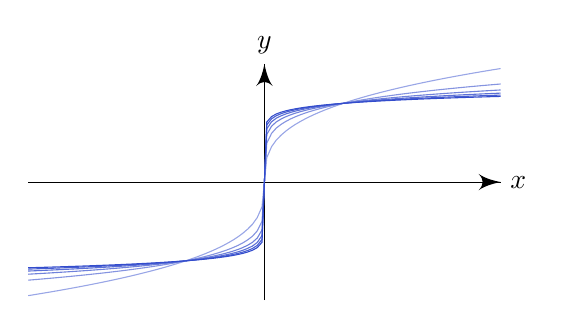
\begin{tikzpicture}
      \draw [->] (-3, 0) -- (3, 0) node [right] {$x$};
      \draw [->] (0, -1.5) -- (0, 1.5) node [above] {$y$};

      \foreach \n in {1,2,3,4,5,6} {
        \pgfmathsetmacro\c{40 + 10 * \n};
        \pgfmathsetmacro\k{1 / (2*\n + 1)};
        \draw [domain=-3:3, samples=100, mblue!\c!white] plot (\x, {\x ^ \k});
      }
    \end{tikzpicture}
  \end{center}
\end{eg}

\begin{eg}
  Let $f_n: [0, 1] \to \R$ be the piecewise linear function formed by joining $(0, 0), (\frac{1}{n}, n), (\frac{2}{n}, 0)$ and $(1, 0)$.
  \begin{center}
    \begin{tikzpicture}
      \draw [->] (0, 0) -- (4, 0) node [right] {$x$};
      \draw [->] (0, 0) -- (0, 3) node [above] {$y$};
      \draw [thick, mred] (0, 0) -- (0.7, 2) -- (1.4, 0) -- (4, 0);
      \node [anchor = north east] {$0$};
      \node at (1.4, 0) [below] {$\frac{2}{n}$};
      \draw [dashed] (0.7, 0) node [below] {$\frac{1}{n}$} -- (0.7, 2) -- (0, 2) node [left] {$n$};
    \end{tikzpicture}
  \end{center}
  The pointwise limit of this function is $f_n(x) \to f(x) = 0$. However, we have
  \[
    \int_0^a f_n(x)\;\d x = 1\text{ for all }n;\quad \int_0^1 f(x) \;\d x = 0.
  \]
  So the limit of the integral is not the integral of the limit.
\end{eg}

\begin{eg}
  Let $f_n: [0, 1] \to \R$ be defined as
  \[
    f_n (x) =
    \begin{cases}
      1 & n!x \in \Z\\
      0 & \text{otherwise}
    \end{cases}
  \]
  Since $f_n$ has finitely many discontinuities, it is Riemann integrable. However, the limit is
  \[
    f_n(x) \to f(x) =
    \begin{cases}
      1 & x\in \Q\\
      0 & x\not\in \Q
    \end{cases}
  \]
  which is not integrable. So integrability of a function is not preserved by pointwise limits.
\end{eg}
This suggests that we need a stronger notion of convergence. Of course, we don't want this notion to be too strong. For example, we could define $f_n \to f$ to mean ``$f_n = f$ for all sufficiently large $n$'', then any property common to $f_n$ is obviously inherited by the limit. However, this is clearly silly since only the most trivial sequences would converge.

Hence we want to find a middle ground between the two cases --- a notion of convergence that is sufficiently strong to preserve most interesting properties, without being too trivial. To do so, we can examine what went wrong in the examples above. In the last example, even though our sequence $f_n$ does indeed tends pointwise to $f$, different points converge at different rates to $f$. For example, at $x = 1$, we already have $f_1(1) = f(1) = 1$. However, at $x = (100!)^{-1}$, $f_{99}(x) = 0$ while $f(x) = 1$. No matter how large $n$ is, we can still find some $x$ where $f_n(x)$ differs a lot from $f(x)$. In other words, if we are given pointwise convergence, there is no guarantee that for very large $n$, $f_n$ will ``look like'' $f$, since there might be some points for which $f_n$ has not started to move towards $f$.

Hence, what we need is for $f_n$ to converge to $f$ at the same pace. This is known as uniform convergence.

\begin{defi}[Uniform convergence]
  A sequence of functions $f_n: E\to \R$ converges \emph{uniformly} to $f$ if
  \[
    (\forall \varepsilon)(\exists N)(\forall x)(\forall n > N)\; |f_n(x) - f(x)| < \varepsilon.
  \]
  Alternatively, we can say
  \[
    (\forall \varepsilon)(\exists N)(\forall n > N)\; \sup_{x\in E} |f_n(x) - f(x)| < \varepsilon.
  \]
\end{defi}
Note that similar to pointwise convergence, the definition does not require $E$ to be a subset of $\R$. It could as well be the set $\{\text{Winnie},\text{Piglet},\text{Tigger}\}$. However, many of our \emph{theorems} about uniform convergence will require $E$ to be a subset of $\R$, or else we cannot sensibly integrate or differentiate our function.

We can compare this definition with the definition of pointwise convergence:
\[
  (\forall \varepsilon)(\forall x)(\exists N)(\forall n > N)\; |f_n(x) - f(x)| < \varepsilon.
\]
The only difference is in where there $(\forall x)$ sits, and this is what makes all the difference. Uniform convergence requires that there is an $N$ that works for \emph{every} $x$, while pointwise convergence just requires that for each $x$, we can find an $N$ that works.

It should be clear from definition that if $f_n \to f$ uniformly, then $f_n \to f$ pointwise. We will show that the converse is false:
\begin{eg}
  Again consider our first example, where $f_n: [-1, 1] \to \R$ is defined by $f_n(x) = x^{1/(2n + 1)}$. If the uniform limit existed, then it must be given by
  \[
    f_n(x) \to f(x) =
    \begin{cases}
      1 & 0 < x \leq 1\\
      0 & x = 1\\
      -1 & -1 \leq x < 0
    \end{cases},
  \]
  since uniform convergence implies pointwise convergence.

  We will show that we don't have uniform convergence. Pick $\varepsilon = \frac{1}{4}$. Then for each $n$, $x = 2^{-(2n + 1)}$ will have $f_n(x) = \frac{1}{2}$, $f(x) = 1$. So there is some $x$ such that $|f_n(x) - f(x)| > \varepsilon$. So $f_n \not\to f$ uniformly.
\end{eg}

\begin{eg}
  Let $f_n: \R \to \R$ be defined by $f_n (x) = \frac{x}{n}$. Then $f_n(x) \to f(x) = 0$ pointwise. However, this convergence is not uniform in $\R$ since $|f_n(x) - f(x)| = \frac{|x|}{n}$, and this can be arbitrarily large for any $n$.

  However, if we restrict $f_n$ to a bounded domain, then the convergence is uniform. Let the domain be $[-a, a]$ for some positive, finite $a$. Then
  \[
    \sup |f_n(x) - f(x)| = \frac{|x|}{n} \leq \frac{a}{n}.
  \]
  So given $\varepsilon$, pick $N$ such that $N > \frac{a}{\varepsilon}$, and we are done.
\end{eg}

Recall that for sequences of normal numbers, we have normal convergence and Cauchy convergence, which we proved to be the same. Then clearly pointwise convergence and pointwise Cauchy convergence of functions are equivalent. We will now look into the case of uniform convergence.

\begin{defi}[Uniformly Cauchy sequence]
  A sequence $f_n: E\to \R$ of functions is \emph{uniformly Cauchy} if
  \[
    (\forall \varepsilon > 0)(\exists N)(\forall m,n > N)\;\sup_{x\in E}|f_n(x) - f_m(x)| < \varepsilon.
  \]
\end{defi}

Our first theorem will be that uniform Cauchy convergence and uniform convergence are equivalent.

\begin{thm}
  Let $f_n: E\to \R$ be a sequence of functions. Then $(f_n)$ converges uniformly if and only if $(f_n)$ is uniformly Cauchy.
\end{thm}

\begin{proof}
  First suppose that $f_n \to f$ uniformly. Given $\varepsilon$, we know that there is some $N$ such that
  \[
    (\forall n > N)\; \sup_{x\in E} |f_n(x) - f(x)| < \frac{\varepsilon}{2}.
  \]
  Then if $n, m > N$, $x\in E$ we have
  \[
    |f_n(x) - f_m(x)| \leq |f_n(x) - f(x)| + |f_m(x) - f(x)| < \varepsilon.
  \]
  So done.

  Now suppose $(f_n)$ is uniformly Cauchy. Then $(f_n(x))$ is Cauchy for all $x$. So it converges. Let
  \[
    f(x) = \lim_{n\to \infty}f_n(x).
  \]
  We want to show that $f_n \to f$ uniformly. Given $\varepsilon > 0$, choose $N$ such that whenever $n, m > N$, $x\in E$, we have $|f_n(x) - f_m(x)| < \frac{\varepsilon}{2}$. Letting $m\to \infty$, $f_m(x) \to f(x)$. So we have $|f_n(x) - f(x)| \leq \frac{\varepsilon}{2} < \varepsilon$. So done.
\end{proof}

This is an important result. If we are given a concrete sequence of functions, then the usual way to show it converges is to compute the pointwise limit and then prove that the convergence is uniform. However, if we are dealing with sequences of functions in general, this is less likely to work. Instead, it is often much easier to show that a sequence of functions is uniformly convergent by showing it is uniformly Cauchy.

We now move on to show that uniform convergence tends to preserve properties of functions.
\begin{thm}[Uniform convergence and continuity]
  Let $E \subseteq \R$, $x \in E$ and $f_n, f: E\to \R$. Suppose $f_n \to f$ uniformly, and $f_n$ are continuous at $x$ for all $n$. Then $f$ is also continuous at $x$.

  In particular, if $f_n$ are continuous everywhere, then $f$ is continuous everywhere.
\end{thm}
This can be concisely phrased as ``the uniform limit of continuous functions is continuous''.

\begin{proof}
  Let $\varepsilon > 0$. Choose $N$ such that for all $n \geq N$, we have
  \[
    \sup_{y\in E}|f_n(y) - f(y)| < \varepsilon.
  \]
  Since $f_N$ is continuous at $x$, there is some $\delta$ such that
  \[
    |x - y| < \delta \Rightarrow |f_N(x) - f_N(y)| < \varepsilon.
  \]
  Then for each $y$ such that $|x - y| < \delta$, we have
  \[
    |f(x) - f(y)| \leq |f(x) - f_N(x)| + |f_N(x) - f_N(y)| + |f_N(y) - f(y)| < 3\varepsilon.
  \]
\end{proof}

\begin{thm}[Uniform convergence and integrals]
  Let $f_n, f: [a, b]\to \R$ be Riemann integrable, with $f_n \to f$ uniformly. Then
  \[
    \int_a^b f_n(t)\;\d t \to \int_a^b f(t)\;\d t.
  \]
\end{thm}

\begin{proof}
  We have
  \begin{align*}
    \left|\int_a^b f_n(t) \;\d t - \int_a^b f(t)\;\d t\right| &= \left|\int_a^b f_n(t) - f(t)\;\d t\right|\\
    &\leq \int_a^b |f_n(t) - f(t)|\;\d t\\
    &\leq \sup_{t\in [a, b]}|f_n(t) - f(t)| (b - a)\\
    &\to 0\text{ as }n\to \infty
  \end{align*}
\end{proof}
This is really the easy part. What we would also want to prove is that if $f_n$ is integrable, $f_n \to f$ uniformly, then $f$ is integrable. This is indeed true, but we will not prove it yet. We will come to this later on at the part where we talk a lot about integrability.

So far so good. However, the relationship between uniform convergence and differentiability is more subtle. The uniform limit of differentiable functions need not be differentiable. Even if it were, the limit of the derivative is not necessarily the same as the derivative of the limit, even if we just want pointwise convergence of the derivative.

\begin{eg}
  Let $f_n, f: [-1, 1] \to \R$ be defined by
  \[
    f_n(x) = |x|^{1 + 1/n}, \quad f(x) = |x|.
  \]
  Then $f_n \to f$ uniformly (exercise).

  Each $f_n$ is differentiable --- this is obvious at $x \not= 0$, and at $x = 0$, the derivative is
  \[
    f_n'(0) = \lim_{x \to 0}\frac{f_n (x) - f_n(0)}{x} = \lim_{x \to 0} \sgn(x) |x|^{1/n} = 0
  \]
  However, the limit $f$ is not differentiable at $x = 0$.
\end{eg}

\begin{eg}
  Let
  \[
    f_n(x) = \frac{\sin nx}{\sqrt{n}}
  \]
  for all $x\in \R$. Then
  \[
    \sup_{x\in \R}|f_n (x)| \leq \frac{1}{\sqrt{n}} \to 0.
  \]
  So $f_n \to f = 0$ uniformly in $\R$. However, the derivative is
  \[
    f_n'(x) = \sqrt{n} \cos nx,
  \]
  which does not converge to $f' = 0$, eg. at $x = 0$.
\end{eg}

Hence, for differentiability to play nice, we need a condition even stronger than uniform convergence.
\begin{thm}
  Let $f_n: [a, b]\to \R$ be a sequence of functions differentiable on $[a, b]$ (at the end points $a$, $b$, this means that the one-sided derivatives exist). Suppose the following holds:
  \begin{enumerate}
    \item For some $c\in [a, b]$, $f_n(c)$ converges.
    \item The sequence of derivatives $(f_n')$ converges uniformly on $[a, b]$.
  \end{enumerate}
  Then $(f_n)$ converges uniformly on $[a, b]$, and if $f = \lim f_n$, then $f$ is differentiable with derivative $f'(x) = \lim f_n'(x)$.
\end{thm}
Note that we do \emph{not} assume that $f_n'$ are continuous or even Riemann integrable. If they are, then the proof is much easier!

\begin{proof}
  If we are given a specific sequence of functions and are asked to prove that they converge uniformly, we usually take the pointwise limit and show that the convergence is uniform. However, given a general function, this is usually not helpful. Instead, we can use the Cauchy criterion by showing that the sequence is uniformly Cauchy.

  We want to find an $N$ such that $n, m> N$ implies $\sup|f_n - f_m| < \varepsilon$. We want to relate this to the derivatives. We might want to use the fundamental theorem of algebra for this. However, we don't know that the derivative is integrable! So instead, we go for the mean value theorem.

  Fix $x\in [a, b]$. We apply the mean value theorem to $f_n - f_m$ to get
  \[
    (f_n - f_m)(x) - (f_n - f_m)(c) = (x - c)(f'_n - f'_m)(t)
  \]
  for some $t\in (x, c)$.

  Taking the supremum and rearranging terms, we obtain
  \[
    \sup_{x\in [a, b]}|f_n(x) - f(x)| \leq |f_n(c) - f_m(c)| + (b - a)\sup_{t\in [a, b]}|f_n'(t) - f_m'(t)|.
  \]
  So given any $\varepsilon$, since $f_n'$ and $f_n(c)$ converge and are hence Cauchy, there is some $N$ such that for any $n, m \geq N$,
  \[
    \sup_{t \in [a, b]} |f_n'(t) - f_m'(t)| < \varepsilon, \quad |f_n(c) - f_m(c)| < \varepsilon.
  \]
  Hence we obtain
  \[
    n, m \geq N \Rightarrow \sup_{x\in [a, b]}|f_n(x) - f_m(x)| < (1 + b - a) \varepsilon.
  \]
  So by the Cauchy criterion, we know that $f_n$ converges uniformly. Let $f = \lim f_n$.

  Now we have to check differentiability. Let $f_n' \to h$. For any fixed $y\in [a, b]$, define
  \[
    g_n(x) =
    \begin{cases}
      \frac{f_n(x) - f_n(y)}{x - y} & x \not= y\\
      f_n'(y) & x = y
    \end{cases}
  \]
  Then by definition, $f_n$ is differentiable at $y$ iff $g_n$ is continuous at $y$. Also, define
  \[
    g(x) =
    \begin{cases}
      \frac{f(x) - f(y)}{x - y} & x \not= y\\
      h(y) & x = y
    \end{cases}
  \]
  Then $f$ is differentiable with derivative $h$ at $y$ iff $g$ is continuous at $y$. However, we know that $g_n \to g$ pointwise on $[a, b]$, and we know that $g_n$ are all continuous. To conclude that $g$ is continuous, we have to show that the convergence is uniform. To show that $g_n$ converges uniformly, we rely on the Cauchy criterion and the mean value theorem.

  For $x \not = y$, we know that
  \[
    g_n(x) - g_m(x) = \frac{(f_n - f_m)(x) - (f_n - f_m)(y)}{x - y} = (f'_n - f'_m)(t)
  \]
  for some $t \in [x, y]$.

  Let $\varepsilon > 0$. Since $f'$ converges uniformly, there is some $N$ such that for all $x\not= y$, $n, m > N$, we have
  \[
    |g_n(x), g_m(x)| \leq \sup |(f'_n - f'_m)(t)| < \varepsilon.
  \]
  For $x = y$, this is still true since $|g_n(y) - g_m(y)| = |f_n'(y) - f_m'(y)|$ by definition. So
  \[
    n, m\geq N \Rightarrow \sup_{[a, b]}|g_n - g_m| < \varepsilon,
  \]
  ie. $g_n$ converges uniformly. Hence the limit function $g$ is continuous, in particular at $x = y$. So $f$ is differentiable at $y$ and $f'(y) = h(y) = \lim f_n'(y)$.
\end{proof}

If we assume additionally that $f_n'$ are continuous, then there is an easy proof of this theorem. By the fundamental theorem of calculus, we have
\[
  f_n(x) = f_n(c) + \int_c^x f_n'(t)\;\d t.\tag{$*$}
\]
Then we get that
\begin{align*}
  \sup_{[a, b]}|f_n(x) - f_m(x)| &\leq |f_n(c) - f_m(c)| + \sup_{x\in [a, b]}\left|\int_c^x (f_n'(t) - f_m'(t))\;\d t\right|\\
  &\leq |f_n(c) - f_m(c)| + (b - a)\sup_{t\in [a, b]}|f_n'(t) - f_m'(t)|\\
  &< \varepsilon
\end{align*}
for sufficiently large $n, m> N$.

So by the Cauchy criterion, $f_n \to f$ uniformly for some function $f: [a, b] \to \R$.

Since the $f_n'$ are continuous, $h = \lim\limits_{n\to \infty} f_n'$ is continuous and hence integrable. Taking the limit of $(*)$, we get
\[
  f(x) = f(c) + \int_c^x h(t)\;\d t.
\]
Then the fundamental theorem of calculus says that $f$ is differentiable and $f'(x) = h(x) = \lim f_n'(x)$. So done.

Finally, we have a small proposition that can come handy.
\begin{prop}\leavevmode
  \begin{enumerate}
    \item Let $f_n, g_n: E\to \R$, be sequences, and $f_n \to f$, $g_n \to g$ uniformly on $E$. Then for any $a, b\in \R$, $af_n + bg_n \to af + bg$ uniformly.
    \item Let $f_n \to f$ uniformly, and let $g: E\to \R$ is bounded. Then $gf_n: E\to \R$ converges uniformly to $gf$.
  \end{enumerate}
\end{prop}

\begin{proof}\leavevmode
  \begin{enumerate}
    \item Easy exercise.
    \item Say $|g(x)| < M$ for all $x\in E$. Then
    \[
      |(gf_n)(x) - (gf)(x)| \leq M |f_n(x) - f(x)|.
    \]
    So
    \[
      \sup_E |gf_n - gf| \leq M \sup_E |f_n - f| \to 0.
    \]
  \end{enumerate}
\end{proof}
Note that (ii) is false without assuming boundedness. An easy example is to take $f_n = \frac{1}{n}$, $x\in \R$, and $g(x) = x$. Then $x_n \to 0$ uniformly, but $(gf_n)(x) = \frac{x}{n}$ does not converge.

\section{Series of functions}
\subsection{Convergence of series}
Recall that in Analysis I, we studied the convergence of a series of numbers. Here we will look at a series of \emph{functions}. The definitions are almost exactly the same.
\begin{defi}[Convergence of series]
  Let $g_n; E \to \R$ be a sequence of functions. Then we say the series $\sum_{n = 1}^\infty g_n$ converges at a point $x \in E$ if the sequence of partial sums
  \[
    f_n = \sum_{j = 1}^ng_j
  \]
  converges at $x$. The series converges uniformly if $f_n$ converges uniformly.
\end{defi}

\begin{defi}[Absolute convergence]
  $\sum g_n$ converges \emph{absolutely} at a point $x\in E$ if $\sum |g_n|$ converges at $x$.

  $\sum g_n$ converges \emph{absolutely uniformly} if $\sum |g_n|$ converges uniformly.
\end{defi}

\begin{prop}
  Let $g_n: E\to \R$. If $\sum g_n$ converges absolutely uniformly, then $\sum g_n$ converges uniformly.
\end{prop}

\begin{proof}
  Again, we don't have a candidate for the limit. So we use the Cauchy criterion.

  Let $f_n = \sum\limits_{j = 1}^n g_j$ and $h_n(x) = \sum\limits_{j = 1}^n |g_j|$ be the partial sums. Then for $n > m$, we have
  \[
    |f_n(x) - f_m(x)| = \left|\sum_{j = m + 1}^n g_j(x)\right| \leq \sum_{j = m + 1}^n |g_j(x)| = |h_n(x) - h_m(x)|.
  \]
  By hypothesis, we have
  \[
    \sup_{x\in E}|h_n(x) - h_m(x)| \to 0\text{ as }n, m\to \infty.
  \]
  So we get
  \[
    \sup_{x\in E}|f_n(x) - f_m(x)| \to 0\text{ as }n, m\to \infty.
  \]
  So the result follows from the Cauchy criteria.
\end{proof}
It is important to remember that uniform convergence plus absolute pointwise convergence does not imply absolute uniform convergence.

\begin{eg}
  Consider the series
  \[
    \sum_{n = 1}^\infty \frac{(-1)^n}{n}x^n.
  \]
  This converges absolutely for every $x\in [0, 1)$ since it is bounded by the geometric series. In fact, it converges \emph{uniformly} on $[0, 1)$ (see example sheet). However, this does \emph{not} converge absolutely uniformly on $[0, 1)$.

  We can consider the difference in partial sums
  \[
    \sum_{j = m}^n \left|\frac{(-1)^j}{j}x^j\right| = \sum_{j = m}^n \frac{1}{j}|x|^j \geq \left(\frac{1}{m} + \frac{1}{m + 1} + \cdots + \frac{1}{n}\right)|x|^n.
  \]
  For each $N$, we can make this difference large enough by picking a really large $n$, and then making $x$ close enough to $1$. So the supremum is unbounded.
\end{eg}

\begin{thm}[Weierstrass M-test]
  Let $g_n: E \to \R$ be a sequence of functions. Suppose there is some sequence $M_n$ such that for all $n$, we have
  \[
    \sup_{x\in E}|g_n (x)| \leq M_n.
  \]
  If $\sum M_n$ converges, then $\sum g_n$ converges absolutely uniformly.
\end{thm}
This is in fact a very easy result, and we could as well reproduce the proof whenever we need it. However, this pattern of proving absolute uniform convergence is so common that we prove it as a test.

\begin{proof}
  Let $f_n = \sum\limits_{j = 1}^n |g_j|$ be the partial sums. Then for $n > m$, we have
  \[
    |f_n(x) - f_m(x)| = \sum_{j = m + 1}^n |g_j(x)| \leq \sum_{j = m + 1}^n M_j.
  \]
  Taking supremum, we have
  \[
    \sup|f_n(x) - f_m(x)| \leq \sum_{j = m + 1}^n M_j \to 0\text{ as }n, m\to \infty.
  \]
  So done by the Cauchy criterion.
\end{proof}

\subsection{Power series}
A particularly interesting kind of series is a \emph{power series}. We have already met these in IA Analysis I and proved some results about them. However, our results were pointwise results, discussing how $\sum c_n (x - a)^n$ behaves at a each particular point $x$. Here we will quickly look into how the power series behaves as a function of $x$. In particular, we want to know whether it converges absolutely uniformly.

\begin{thm}
  Let $\sum\limits_{n = 0}^\infty c_n (x - a)^n$ be a real power series. Then there exists a unique number $R\in [0, +\infty]$ (called the radius of convergence) such that
  \begin{enumerate}
    \item If $|x - a| < R$, then $\sum c_n (x - a)^n$ converges absolutely.
    \item If $|x - a| > R$, then $\sum c_n (x - a)^n$ diverges.
    \item If $R > 0$ and $0 < r < R$, then $\sum c_n (x - a)^n$ converges absolutely uniformly on $[a - r, a + r]$.

      We say that the sum converges locally absolutely uniformly inside circle of convergence, ie. for every point $y\in (a - R, a + R)$, there is some open interval around $y$ on which the sum converges absolutely uniformly.
  \end{enumerate}
  These results hold for complex power series as well, but for concreteness we will just do it for real series.
\end{thm}
Note that the first two statements are things we already know from IA Analysis I, and we are not going to prove them.
\begin{proof}
  See IA Analysis I for (i) and (ii).

  For (iii), note that from (i), taking $x = a - r$, we know that $\sum |c_n| r^n$ is convergent. But we know that if $x\in [a - r, a + r]$, then
  \[
    |c_n (x - a)^n| \leq |c_n| r^n.
  \]
  So the result follows from the Weierstrass M-test by taking $M_n = |c_n| r^n$.
\end{proof}
Note that uniform convergence need not hold on the entire interval of convergence.
\begin{eg}
  Consider $\sum x^n$. This converges for $x\in (-1, 1)$, but uniform convergence fails on $(-1, 1)$ since the tail
  \[
    \sum_{j = m}^n x^j = x^n \sum_{j = 0}^{n - m} x^j \geq \frac{x^m}{1 - x}.
  \]
  This is not uniformly small since we can make this large by picking $x$ close to $1$.
\end{eg}

\begin{thm}[Termwise differentiation of power series]
  Suppose $\sum c_n (x - n)^n$ is a real power series with radius of convergence $R > 0$. Then
  \begin{enumerate}
    \item The ``derived series''
      \[
        \sum_{n = 1}^\infty n c_n (x - a)^{n - 1}
      \]
      has radius of convergence $R$.
    \item The function defined by $f(x) = \sum c_n (x - a)^n$, $x\in (a - R, a + R)$ is differentiable with derivative $f'(x) = \sum n c_n (x - a)^{n - 1}$ within the (open) circle of convergence.
  \end{enumerate}
\end{thm}

\begin{proof}\leavevmode
  \begin{enumerate}
    \item Let $R_1$ be the radius of convergence of the derived series. We know
      \[
        |c_n(x - a)^n| = |c_n||x - a|^{n - 1}|x - a| \leq |n c_n (x - a)^{n - 1}| |x - a|.
      \]
      Hence if the derived series $\sum n c_n(x - a)^{n - 1}$ converges absolutely for some $x$, then so does $\sum c_n (x - a)^n$. So $R_1 \leq R$.

      Suppose that the inequality is strict, ie. $R_1 < R$, then there are $r_1, r$ such that $R_1 < r_1 < r < R$, where $\sum n|c_n| r_1^{n - 1}$ diverges while $\sum |c_n| r^n$ converges. But this cannot be true since $n|c_n| r_1^{n - 1} \leq |c_n| r^n$ for sufficiently large $n$. So we must have $R_1 = R$.

    \item Let $f_n(x) = \sum\limits_{j = 0}^n c_j (x - a)^j$. Then $f_n '(x) = \sum\limits_{j = 1}^n j c_j (x - a)^{j - 1}$. We want to use the result that the derivative of limit is limit of derivative. This requires that $f_n$ converges at a point, and that $f_n'$ converges uniformly. The first is obviously true, and we know that $f_n'$ converges uniformly on $[a - r, a + r]$ for any $r < R$. So for each $x_0$, there is some interval containing $x_0$ on which $f_n'$ is convergent. So on this interval, we know that
      \[
        f(x) = \lim_{n \to \infty}f_n (x)
      \]
      is differentiable with
      \[
        f'(x) = \lim_{n \to \infty}f_n'(x) = \sum_{j = 1}^\infty jc_j (x - a)^j.
      \]
      In particular,
      \[
        f'(x_0) = \sum_{j = 1}^\infty jc_j (x_0 - a)^j.
      \]
      Since this is true for all $x_0$, the result follows.
  \end{enumerate}
\end{proof}

\section{Uniform continuity and integration}
\subsection{Uniform continuity}
Recall that we had a rather weak notion of convergence, known as pointwise convergence, and then promoted it to \emph{uniform convergence}. The process of this promotion is to replace the condition ``for each $x$, we can find an $\varepsilon$'' to ``we can find an $\varepsilon$ that works for each $x$''. We are going to do the same for continuity to obtain uniform continuity.

\begin{defi}[Uniform continuity]
  Let $E \subseteq \R$ and $f: E\to \R$. We say that $f$ is \emph{uniformly continuous} on $E$ if
  \[
    (\forall \varepsilon)(\exists \delta > 0)(\forall x)(\forall y)\; |x - y| < \delta \Rightarrow |f(x) - f(y)| < \varepsilon.
  \]
\end{defi}
Compare this to the definition of continuity:
\[
  (\forall \varepsilon)(\forall x)(\exists \delta > 0)(\forall y)\; |x - y| < \delta \Rightarrow |f(x) - f(y)| < \varepsilon.
\]
Again, we have shifted the $(\forall x)$ out of the $(\exists \delta)$ quantifier. The difference is that in regular continuity, $\delta$ can depend on our choice of $x$, but in uniform continuity, it only depends on $y$. Again, clearly a uniformly continuous function is continuous.

In general, the converse is not true, as we will soon see in two examples. However, the converse is true in a lot of cases.
\begin{thm}
  Any continuous function on a closed, bounded interval is uniformly continuous.
\end{thm}

\begin{proof}
  We are going to prove by contradiction. Suppose $f: [a, b] \to \R$ is not uniformly continuous. Since $f$ is not uniformly continuous, there is some $\varepsilon > 0$ such that for all $\delta = \frac{1}{n}$, there is some $x_n, y_n$ such that $|x_n - y_n| < \frac{1}{n}$ but $|f(x_n) - f(y_n)| > \varepsilon$.

  Since we are on a closed, bounded interval, by Bolzano-Weierstrass, $(x_n)$ has a convergent subsequence $(x_{n_i}) \to x$. Then we also have $y_{n_i}\to x$. So by continuity, we must have $f(x_{n_i}) \to f(x)$ and $f(y_{n_i}) \to f(x)$. But $|f(x_{n_i}) - f(y_{n_i})| > \varepsilon$ for all $n_i$. This is a contradiction.
\end{proof}
Note that we proved this in the special case where the domain is $[a, b]$ and the image is $\R$. In fact, $[a, b]$ can be replaced by any compact metric space; $\R$ by any metric space. This is since all we need is for Bolzano-Weierstrass to hold in the domain, ie. the domain is sequentially compact (ignore this comment if you have not taken IB Metric and Topological Spaces).

Instead of a contradiction, we can also do a direct proof of this statement, using the Heine-Borel theorem which says that $[0, 1]$ is compact.

While this is a nice theorem, in general a continuous function need not be uniformly continuous.

\begin{eg}
  Consider $f: (0, 1] \to \R$ given by $f(x) = \frac{1}{x}$. This is not uniformly continuous, since when we get very close to $0$, a small change in $x$ produces a large change in $\frac{1}{x}$.

  In particular, for any $\delta < 1$ and $x < \delta$, $y = \frac{x}{2}$, then $|x - y| = \frac{x}{2} < \delta$ but $|f(x) - f(y)| = \frac{1}{x} > 1$.
\end{eg}

In this example, the function is unbounded. However, even bounded functions can be not uniformly continuous.
\begin{eg}
  Let $f: (0, 1] \to \R$, $f(x) = \sin \frac{1}{x}$. We let
  \[
    x_n = \frac{1}{2n\pi},\quad y_n = \frac{1}{(2n + \frac{1}{2})\pi}.
  \]
  Then we have
  \[
    |f(x_n) - f(y_n)| = |0 - 1| = 1,
  \]
  while
  \[
    |x_n - y_n| = \frac{\pi}{2n(4n + 1)} \to 0.
  \]
\end{eg}

\subsection{Applications to Riemann integrability}
We can apply the idea of uniform continuity to Riemann integration.

We first quickly recap and summarize things we know about Riemann integrals IA Analysis I. Let $f: [a, b] \to \R$ be a bounded function, say $m \leq f(x) \leq M$ for all $x\in [a, b]$. Consider a partition of $[a, b]$
\[
  P = \{a_0, a_1, \cdots, a_n\}.
\]
ie. $a = a_0 < a_1 < a_2 < \cdots < a_n = b$. The \emph{upper sum} is defined as
\[
  U(P, f) = \sum_{j = 0}^{n - 1} (a_{j + 1} - a_j) \sup_{[a_j, a_{j + 1}]} f.
\]
Similarly, the lower sum is defined as
\[
  L(P, f) = \sum_{j = 0}^{n - 1} (a_{j + 1} - a_j) \inf_{[a_j, a_{j + 1}]} f.
\]
It is clear from definition that
\[
  m(b - a) \leq L(P, f) \leq U(P, f) \leq M(b - a).
\]
Also, if a partition $P^*$ is a \emph{refinement} of a partition $P$, ie. it contains all the points of $P$ and possibly more, then
\[
  L(P, f) \leq L(P^*, f) \leq U(P^*, f) \leq U(P, f).
\]
It thus follow that if $P_1$ and $P_2$ are arbitrary partitions, then
\[
  L(P_1, f) \leq L(P_2, f),
\]
which we can show by finding a partition that is simultaneously a refinement of $P_1$ and $P_2$. The importance of this result is that
\[
  \sup_{P} L(P, f) \leq \inf_P U(P, f),
\]
where we take extrema over all partitions $P$. We define these to be the \emph{upper and lower integrals}
\[
  I^*(f) = \inf_P U(P, f),\quad I_*(f) = \sup_P L(p, f).
\]
So we know that
\[
  m(b - a) \leq I_*(f) \leq I^*(f) \leq M(b - a).
\]
Now given any $\varepsilon > 0$, by definition of the infimum, there is a partition $P_1$ such that
\[
  U(P_1, f) < I^*(f) + \frac{\varepsilon}{2}.
\]
Similarly, there is a partition $P_2$ such that
\[
  L(P_2, f) > I_*(f) - \frac{\varepsilon}{2}.
\]
So if we let $P = P_1 \cup P_2$, then $P$ is a refinement of both $P_1$ and $P_2$. So
\[
  U(P_f) < I^*(f) + \frac{\varepsilon}{2}
\]
and
\[
  L(P, f) > I_*(f) - \frac{\varepsilon}{2}.
\]
Combining these, we know that
\[
  0 \leq I^*(f) - I_*(f) < U(P, f) - L(P, f) < I^*(f) - I_*(f) + \varepsilon.
\]
We now define what it means to be Riemann integrable.
\begin{defi}[Riemann integrability]
  A bounded function $f: [a, b] \to \R$ is \emph{Riemann integrable} on $[a, b]$ if $I^*(f) = I_*(f)$. We write
  \[
    \int_a^b f(x)\;\d x = I^*(f) = I_*(f).
  \]
\end{defi}

Then the Riemann criterion says
\begin{thm}[Riemann criterion for integrability]
  A bounded function $f: [a, b] \to \R$ is Riemann integrable if and only if for every $\varepsilon$, there is a partition $P$ such that
  \[
    U(P, f) - L(P, f) < \varepsilon.
  \]
\end{thm}
That's the end of our recap. Now we have a new theorem.

\begin{thm}
  If $f: [a, b] \to [A, B]$ is integrable and $g: [A, B] \to \R$ is continuous, then $g\circ f: [a, b] \to \R$ is integrable.
\end{thm}

\begin{proof}
  Let $\varepsilon > 0$. Since $g$ is continuous, $g$ is uniformly continuous. So we can find $\delta = \delta(\varepsilon) > 0$ such that for any $x, y\in [A, B]$ such that $|x - y| < \delta$, then $|g(x) - g(y)| < \varepsilon$.

  Since $f$ is integrable, for arbitrary $\varepsilon'$, we can find a partition $P = \{a = a_0 < a_1 < \cdots < a_n = b\}$ such that
  \[
    U(P, f) - L(P, f) = \sum_{j = 0}^{n - 1} (a_{j + 1} - a_j) \left(\sup_{I_j} f - \inf_{I_j} f\right) < \varepsilon'. \tag{$*$}
  \]
  Our objective is to make $U(P, g\circ f) - L(P, g\circ f)$ small. By uniform continuity of $g$, if $\sup_{I_j} f - \inf_{I_j} f$ is less than $\delta$, then $\sup_{I_j} g\circ f - \inf_{I_j} g\circ f$ will be less that $\varepsilon$. We like these sorts of intervals. So we let
  \[
    J = \left\{j: \sup_{I_j} f - \inf_{I_j}f < \delta\right\},
  \]
  We now show properly that these intervals are indeed ``nice''. For any $j \in J$, for all $x, y\in I_j$, we must have
  \[
    |f(x) - f(y)| \leq \sup_{z_1, z_2\in I_j} (f(z_1) - f(z_2)) = \sup_{I_j} f - \inf_{I_j} f < \delta.
  \]
  Hence, for each $j\in J$ and all $x, y\in I_j$, we know that
  \[
    |g\circ f(x) - g\circ f(y)| < \varepsilon.
  \]
  Hence, we must have
  \[
    \sup_{I_j} \Big(g\circ f(x) - g\circ f(y)\Big) \leq \varepsilon.
  \]
  So
  \[
    \sup_{I_j} g\circ f - \inf_{I_j} g\circ f \leq \varepsilon.
  \]
  Hence we know that
  \begin{align*}
    U(P, g\circ f) - L(P, g\circ f) &= \sum_{j = 0}^n (a_{j + 1} - a_j) \left(\sup_{I_j}g\circ f - \inf_{I_j}g\circ f\right)\\
    &= \sum_{j \in J} (a_{j + 1} - a_j) \left(\sup_{I_j}g\circ f - \inf_{I_j}g\circ f\right) \\
    &\quad\quad\quad+ \sum_{j \not\in J} (a_{j + 1} - a_j)\left(\sup_{I_j}g\circ f - \inf_{I_j}g\circ f\right).\\
    &\leq \varepsilon(b - a) + 2\sup_{[A, B]}|g| \sum_{j\not\in J}(a_{j + 1} - a_j).
  \end{align*}
  Hence, it suffices here to make $\sum\limits_{j\not\in J} (a_{j + 1} - a_j)$ small. From $(*)$, we know that we must have
  \[
    \sum_{j \not\in J} (a_{j + 1} - a_j) < \frac{\varepsilon'}{\delta},
  \]
  or else $U(p, f) - L(P, f) > \varepsilon'$. So we can bound
  \[
    U(P, g\circ f) - L(P, g\circ f) \leq \varepsilon(b - a) + 2\sup_{[A, B]} \frac{\varepsilon'}{\delta}.
  \]
  So if we are given an $\varepsilon$ at the beginning, we can get a $\delta$ by uniform continuity. Afterwards, we pick $\varepsilon'$ such that $\varepsilon' = \varepsilon \delta$. Then we have shown that given any $\varepsilon$, there exists a partition such that
  \[
    U(P, g\circ f) - L(P, g\circ f) < \left((b - a) + 2\sup_{[A, B]} |g|\right) \varepsilon.
  \]
  Then the claim follows from the Riemann criterion.
\end{proof}

As an immediate consequence, we know that any continuous function is integrable, since we can just let $f$ be the identity function, which we can easily show to be integrable.

\begin{cor}
  A continuous function $g:[a, b] \to \R$ is integrable.
\end{cor}

\begin{thm}
  Let $f_n: [a, b] \to \R$ be bounded and integrable for all $n$. Then if $(f_n)$ converges uniformly to a function $f: [a ,b] \to \R$, then $f$ is bounded and integrable.
\end{thm}

\begin{proof}
  Let
  \[
    c_n = \sup_{[a, b]} |f_n - f|.
  \]
  Then uniform convergence says that $c_n \to 0$. By definition, for each $x$, we have
  \[
    f_n(x) - c_n \leq f(x) \leq f_n(x) + c_n.
  \]
  Since $f_n$ is bounded, this implies that $f$ is bounded by $\sup |f_n| + c_n$. Also, for any $x, y\in [a, b]$, we know
  \[
    f(x) - f(n) \leq (f_n(x) - f(n)) + 2 c_n.
  \]
  Hence for any partition $P$,
  \[
    U(P, f) - L(L, f) \leq U(P, f_n) - L(P, f_n) + 2(b - a) c_n.
  \]
  So given $\varepsilon > 0$, first choose $n$ such that $2(b - a) c_n < \frac{\varepsilon}{2}$. Then choose $P$ such that $U(P, f_n) - L(P, f_n) < \frac{\varepsilon}{2}$. Then for this partition, $U(P, f) - L(P, f) < \varepsilon$.
\end{proof}

Most of the theory of Riemann integration extends to vector-valued or complex-valued functions (of a single real variable).
\begin{defi}[Riemann integrability of vector-valued function]
  Let $\mathbf{f}: [a, b] \to \R^n$ be a vector-valued function. Write
  \[
    \mathbf{f}(x) = (f_1(x), f_2(x), \cdots, f_n(x))
  \]
  for all $x\in [a, b]$. Then $\mathbf{f}$ is \emph{Riemann integrable} iff $f_j: [a, b] \to \R$ is integrable for all $j$. The integral is defined as
  \[
    \int_a^b \mathbf{f}(x)\;\d x = \left(\int_a^b f_1(x)\;\d x, \cdots, \int_a^b f_n(x)\;\d x\right) \in \R^n.
  \]
\end{defi}
It is easy to see that most basic properties of integrals of real functions extend to the vector-valued case. A less obvious fact is the following.
\begin{prop}
  If $\mathbf{f}: [a, b] \to \R^n$ is integrable, then the function $\|\mathbf{f}\|: [a, b] \to \R$ defined by
  \[
    \|\mathbf{f}\|(x) = \|\mathbf{f}(x)\| = \sqrt{\sum_{j = 1}^n f_j^2(x)}.
  \]
  is integrable, and
  \[
    \left\|\int_a^b \mathbf{f}(x)\;\d x\right\| \leq \int_a^b \|\mathbf{f}\|(x)\;\d x.
  \]
\end{prop}
This is a rather random result, but we include it here because it will be helpful at some point in time.

\begin{proof}
  The integrability of $\|\mathbf{f}\|$ is clear since squaring and taking square roots are continuous, and a finite sum of integrable functions is integrable. To show the inequality, we let
  \[
    \mathbf{v} = (v_1, \cdots, v_n) = \int_a^b \mathbf{f}(x)\;\d x.
  \]
  Then by definition,
  \[
    v_j = \int_a^b f_j(x)\;\d x.
  \]
  If $\mathbf{v} = \mathbf{0}$, then we are done. Otherwise, we have
  \begin{align*}
    \|\mathbf{v}\|^2 &= \sum_{j = 1}^n v_j^2 \\
    &= \sum_{j = 1}^n v_j \int_a^b f_j(x)\;\d x \\
    &= \int_a^b \sum_{j = 1}^n (v_j f_j(x))\;\d x\\
    &= \int_a^b \mathbf{v}\cdot \mathbf{f}(x)\;\d x\\
    \intertext{Using the Cauchy-Schwarz inequality, we get}
    &\leq \int_a^b \|\mathbf{v}\| \|\mathbf{f}\|(x)\;\d x\\
    &= \|\mathbf{v}\|\int_a^b \|\mathbf{f}\|\;\d x.
  \end{align*}
  Divide by $\|\mathbf{v}\|$ and we are done.
\end{proof}
\subsection{Non-examinable fun*}
Since there is time left in the lecture, we'll write down a really remarkable result.
\begin{thm}[Weierstrass Approximation Theorem*]
  If $f: [0, 1] \to \R$ is continuous, then there exists a sequence of polynomials $(p_n)$ such that $p_n \to f$ uniformly. In fact, the sequence can be given by
  \[
    p_n(x) = \sum_{k = 0}^n f\left(\frac{i}{n}\right) \binom{n}{k} x^k(1 - x)^{n - k}.
  \]
  These are known as \emph{Bernstein polynomials}.
\end{thm}
Of course, there are many different sequences of polynomials converging uniformly to $f$. Apart from the silly examples like adding $\frac{1}{n}$ to each $p_n$, there can also be vastly different ways of constructing such polynomial sequences.

\begin{proof}
  For convenience, let
  \[
    p_{n, k}(x) = \binom{n}{k}x^k (1 - x)^{n - k}.
  \]
  First we need a few facts about these functions. Clearly, $p_{n, k}(x) \geq 0$ for all $x\in [0, 1]$. Also, by the binomial theorem,
  \[
    \sum_{k = 0}^n \binom{n}{k}x^k y^{n - k} = (x + y)^n.
  \]
  So we get
  \[
    \sum_{k = 0}^n p_{n, k}(x) = 1.
  \]
  Differentiating the binomial theorem with respect to $x$ and putting $y = 1 - x$ gives
  \[
    \sum_{k = 0}^n \binom{n}{k}k x^{k - 1}(1 - x)^{n - k} = n.
  \]
  We multiply by $x$ to obtain
  \[
    \sum_{k = 0}^n \binom{n}{k}k x^k(1 - x)^{n - k} = nx.
  \]
  In other words,
  \[
    \sum_{k = 0}^n kp_{n, k}(x) = nx.
  \]
  Differentiating once more gives
  \[
    \sum_{k = 0}^n k(k - 1)p_{n, k}(x) = n(n - 1)x^2.
  \]
  Adding these two results gives
  \[
    \sum_{k = 0}^n k^2 p_{n, k}(x) = n^2 x^2 + nx(1 - x).
  \]
  We will write our results in a rather weird way:
  \[
    \sum_{k = 0}^n (nx - k)^2 p_{n, k}(x) = n^2 x^2 - 2nx \cdot nx + n^2 x^2 + nx(1 - x) = nx(1 - x).\tag{$*$}
  \]
  This is what we really need.

  Now given $\varepsilon$, since $f$ is continuous, $f$ is uniformly continuous. So pick $\delta$ such that $|f(x) - f(y)| < \varepsilon$ whenever $|x - y| < \delta$.

  Since $\sum p_{n, k}(x) = 1$, $f(x) = \sum p_{n, k}(x) f(x)$. Now for each \emph{fixed} $x$, we can write
  \begin{align*}
    |p_n(x) - f(x)| &= \left|\sum_{k = 0}^n \left(f\left(\frac{k}{n}\right) - f(x)\right) p_{n, k}(x)\right|\\
    &\leq \sum_{k = 0}^n \left|f\left(\frac{k}{n}\right) - f(x)\right| p_{n, k}(x)\\
    &= \sum_{k: |x - k/n| < \delta}\left(\left|f\left(\frac{k}{n}\right) - f(x)\right| p_{n, k}(x)\right) \\
    &\quad\quad\quad+ \sum_{k: |x - k/n| \geq \delta}\left(\left|f\left(\frac{k}{n}\right) - f(x)\right| p_{n, k}(x)\right)\\
    &\leq \varepsilon \sum_{k = 0}^n p_{n, k}(x) + 2\sup_{[0, 1]} |f| \sum_{k: |x - k/n| > \delta} p_{n, k}(x)\\
    &\leq \varepsilon + 2\sup_{[0, 1]} |f|\cdot \frac{1}{\delta^2}\sum_{k: |x - k/n| > \delta} \left(x - \frac{k}{n}\right)^2 p_{n, k}(x)\\
    &\leq \varepsilon + 2\sup_{[0, 1]} |f|\cdot \frac{1}{\delta^2}\sum_{k = 0}^n \left(x - \frac{k}{n}\right)^2 p_{n, k}(x)\\
    &= \varepsilon + \frac{2\sup|f|}{\delta^2 n^2} nx(1 - x)\\
    &\leq \varepsilon + \frac{2\sup|f|}{\delta^2 n}
  \end{align*}
  Hence given any $\varepsilon$ and $\delta$, we can pick $n$ sufficiently large that that $|p_n(x) - f(x)| < 2\varepsilon$. This is picked independently of $x$. So done.
\end{proof}

Unrelatedly, we might be interested in the question --- when is a function Riemann integrable? A possible answer is if it satisfies the Riemann integrability criterion, but this is not really helpful. We know that a function is integrable if it is continuous. But it need not be. It could be discontinuous at finitely many points and still be integrable. If it has countably many discontinuities, then we still can integrate it. How many points of discontinuity can we accommodate if we want to keep integrability?

To answer this questions, we have Lebesgue's theorem. To state this theorem, we need the following definition:
\begin{defi}[Lebesgue measure zero*]
  A subset $A\subseteq \R$ is said to have \emph{(Lebesgue) measure zero} if for any $\varepsilon > 0$, there exists a countable (possibly finite) collection of open intervals $I_j$ such that
  \[
    A \subseteq \bigcup_{j = 1}^\infty I_J,
  \]
  and
  \[
    \sum_{j = 1}^\infty | I_j| < \varepsilon.
  \]
  here $|I_j|$ is defined as the length of the interval, not the cardinality (obviously).
\end{defi}
This is a way to characterize ``small'' sets, and in general a rather good way. This will be studied in depth in the IID Probability and Measure course.

\begin{eg}\leavevmode
  \begin{itemize}
    \item The empty set has measure zero.
    \item Any finite set has measure zero.
    \item Any countable set has measure zero. If $A = \{a_0, a_1, \cdots\}$, take
      \[
        I_j = \left(a_j - \frac{\varepsilon}{2^{j + 1}}, a_j + \frac{\varepsilon}{2^{j + 1}}\right).
      \]
      Then $A$ is contained in the union and the sum of lengths is $\varepsilon$.
    \item A countable union of sets of measure zero has measure zero, using a similar proof strategy as above.
    \item Any (non-trivial) interval does not have measure zero.
    \item The Cantor set, despite being uncountable, has measure zero. The Cantor set is constructed as follows: start with $C_0 = [0, 1]$. Remove the middle third $\left(\frac{1}{3}, \frac{2}{3}\right)$ to obtain $C_1 = \left[0, \frac{1}{3}\right] \cup \left[\frac{2}{3}, 1\right]$. Removing the middle third of each segment to obtain
      \[
        C_2 = \left[0, \frac{1}{9}\right] \cup \left[\frac{2}{9}, \frac{3}{9}\right] \cup \left[\frac{6}{9}, \frac{7}{9}\right]\cup \left[\frac{8}{9}, 1\right].
      \]
      Continue iteratively by removing the middle thirds of each part. Define
      \[
        C = \bigcap_{n = 0}^\infty C_n,
      \]
      which is the Cantor set. Since each $C_n$ consists of $2^n$ disjoint closed intervals of length $1/3^n$, the total length of the segments of $C_n$ is $\left(\frac{2}{3}\right)^n \to 0$. So we can cover $C$ by arbitrarily small union of intervals. Hence the Cantor set has measure zero.

      It is slightly trickier to show that $C$ is uncountable, and to save time, we are not doing it now.
  \end{itemize}
\end{eg}
Using this definition, we can have the following theorem:
\begin{thm}[Lebesgue's theorem on the Riemann integral*]
  Let $f: [a, b] \to \R$ be a bounded function, and let $\mathcal{D}_f$ be the set of points of discontinuities of $f$. Then $f$ is Riemann integrable \emph{if and only if} $\mathcal{D}_f$ has measure zero.
\end{thm}
Using this result, a lot of our theorems follow easily of these. Apart from the easy ones like the sum and product of integrable functions is integrable, we can also easily show that the composition of a continuous function with an integrable function is integrable, since composing with a continuous function will not introduce more discontinuities.

Similarly, we can show that the uniform limit of integrable functions is integrable, since the points of discontinuities of the uniform limit is at most the (countable) union of all discontinuities of the functions in the sequence.

Proof is left as an exercise for the reader, in the example sheet.

\section{\texorpdfstring{$\R^n$}{Rn} as a normed space}
\subsection{Normed spaces}
Our objective is to extend most of the notions we had about functions of a single variable $f: \R \to \R$ to functions of multiple variables $f: \R^n \to \R$. More generally, we want to study functions $f: \Omega \to \R^m$, where $\Omega \subseteq \R^n$. We wish to define analytic notions such as continuity, differentiability and even integrability (even though we are not doing integrability in this course).

In order to do this, we need more structure on $\R^n$. We already know that $\R^n$ is a vector space, which means that we can add, subtract and multiply by scalars. But to do analysis, we need something to replace our notion of $|x - y|$ in $\R$. This is known as a \emph{norm}.

It is useful to define and study this structure in an abstract setting, as opposed to thinking about $\R^n$ specifically. This leads to the general notion of \emph{normed spaces}.

\begin{defi}[Normed space]
  Let $V$ be a real vector space. A \emph{norm} on $V$ is a function $\|\ph \|: V\to \R$ satisfying
  \begin{enumerate}
    \item $\|\mathbf{x}\| \geq 0$ with equality iff $\mathbf{x} = \mathbf{0}$ \hfill (non-negativity)
    \item $\|\lambda \mathbf{x}\| = |\lambda|\|\mathbf{x}\|$ \hfill (linearity in scalar multiplication)
    \item $\|\mathbf{x} + \mathbf{y}\| \leq \|\mathbf{x} \| + \|\mathbf{y}\|$ \hfill (triangle inequality)
  \end{enumerate}
  A \emph{normed space} is a pair $(V, \|\ph \|)$. If the norm is understood, we just say $V$ is a normed space. We do have to be slightly careful since there can be multiple norms on a vector space.
\end{defi}
Intuitively, $\|\mathbf{x}\|$ is the \emph{length} or \emph{magnitude} of $\mathbf{x}$.
\begin{eg}
  We will first look at finite-dimensional spaces. This is typically $\R^n$ with different norms.
  \begin{itemize}
    \item Consider $\R^n$, with the Euclidean norm
      \[
        \|\mathbf{x}\|_2 = \left(\sum x_i^2\right)^2.
      \]
      This is also known as the \emph{usual norm}. It is easy to check that this is a norm, apart from the triangle inequality. So we'll just do this. We have
      \begin{align*}
        \|\mathbf{x} + \mathbf{y}\|^2 &= \sum_{i = 1}^n (x_i + y_i)^2 \\
        &= \|\mathbf{x}\|^2 + \|\mathbf{y}\|^2 + 2\sum x_i y_i \\
        &\leq \|\mathbf{x}\|^2 + \|\mathbf{y}\|^2 + 2\|\mathbf{x}\|\mathbf{y}\| \\
        &= (\|\mathbf{x}\|^2 + \|\mathbf{y}\|^2),
      \end{align*}
      where we used the Cauchy-Schwarz inequality. So done.
    \item We can have the following norm on $\R^n$:
      \[
        \|\mathbf{x}\|_1 = \sum |x_i|.
      \]
      It is easy to check that this is a norm.
    \item We can also have the following norm on $\R^n$:
      \[
        \|\mathbf{x}\|_\infty = \max\{|x_i|: 1 \leq i \leq n\}.
      \]
      It is also easy to check that this is a norm.
    \item In general, we can define the $p$ norm (for $p \geq 1$) by
      \[
        \|\mathbf{x}\|_p = \left(\sum |x_i|^p\right)^{1/p}.
      \]
      It is, however, not trivial to check the triangle inequality, and we will not do this.

      We can show that as $p\to \infty$, $\|\mathbf{x}\|_p \to \|\mathbf{x}\|_\infty$, which justifies our notation above.
  \end{itemize}
  We also have some infinite dimensional examples. Often, we can just extend our notions on $\R^n$ to infinite sequences with some care. We write $\R^\N$ for the set of all infinite real sequences $(x_k)$. This is a vector space with termwise addition and scalar multiplication.
  \begin{itemize}
    \item Define
      \[
        \ell^1 = \left\{(x_k) \in \R^\N: \sum |x_k| < \infty\right\}.
      \]
      This is a linear subspace of $\R^\N$. We define the norm by
      \[
        \|(x_k)\|_1 = \|(x_k)\|_{\ell^1} = \sum |x_k|.
      \]
    \item Similarly, we can define $\ell^2$ by
      \[
        \ell^2 = \left\{(x_k) \in \R^\N: \sum x_k^2 < \infty\right\}.
      \]
      The norm is defined by
      \[
        \|(x_k)\|_2 = \|(x_k)\|_{\ell^2} = \left(\sum x_k^2\right)^{1/2}.
      \]
      We can also write this as
      \[
        \|(x_k)\|_{\ell^2} = \lim_{n \to \infty} \|(x_1, \cdots, x_n)\|_2.
      \]
      So the triangle inequality for the Euclidean norm implies the triangle inequality for $\ell^2$.
    \item In general, for $p \geq 1$, we can define
      \[
        \ell^p = \left\{(x_k) \in \R^\N: \sum |x_k|^p < \infty\right\}
      \]
      with the norm
      \[
        \|(x_k)\|_p = \|(x_k)\|_{\ell^p} = \left(\sum |x_k|^p\right)^{1/p}.
      \]
    \item Finally, we have $\ell^\infty$, where
      \[
        \ell^\infty = \{(x_k)\in \R^\N: \sup |x_k| < \infty\},
      \]
      with the norm
      \[
        \|(x_k)\|_\infty = \|(x_k)\|_{\ell^\infty} = \sup |x_k|.
      \]
  \end{itemize}
  Finally, we can have examples where we look at function spaces, usually $C([a, b])$, the set of continuous real functions on $[a, b]$.
  \begin{itemize}
    \item We can define the $L^1$ norm by
      \[
        \|f\|_{L^1} = \|f\|_1 = \int_a^b |f|\;\d x.
      \]
    \item We can define $L^2$ similarly by
      \[
        \|f\|_{L^2} = \|f\|_2 = \left(\int_a^b f^2 \;\d x\right)^{\frac{1}{2}}.
      \]
    \item In general, we can define $L^p$ for $p \geq 1$ by
      \[
        \|f\|_{L^p} = \|f\|_p = \left(\int_a^b f^p \;\d x\right)^{\frac{1}{p}}.
      \]
    \item Finally, we have $L^\infty$ by
      \[
        \|f\|_{L^\infty} = \|f\|_\infty = \sup |f|.
      \]
      This is also called the \emph{uniform norm}, or the \emph{supremum norm}.
  \end{itemize}
\end{eg}
Later, when we define convergence for general normed space, we will show that convergence under the uniform norm is equivalent to uniform convergence.

To show that $L^2$ is actually a norm, we can use the Cauchy-Schwarz inequality for integrals.
\begin{lemma}[Cauchy-Schwarz inequality (for integrals)]
  If $f, g\in C([a, b])$, $f, g \geq 0$, then
  \[
    \int_a^b fg\;\d x \leq \left(\int_a^b f^2\;\d x)\right)^{1/2}\left(\int_a^b g^2\;\d x\right)^{1/2}.
  \]
\end{lemma}

\begin{proof}
  If $\int_a^b f^2\;\d x = 0$, then $f = 0$ (since $f$ is continuous). So the inequality holds trivially.

  Otherwise, let $A^2 = \int_a^b f^2\;\d x \not= 0$, $B^2 = \int_a^b g^2\;\d x$. Consider the function
  \[
    \phi(t) = \int_a^b (g - tf)^2 \;\d t \geq 0.
  \]
  for every $t$. We can expand this as
  \[
    \phi(t) = t^2 A^2 - 2t \int_a^b gf\;\d x + B^2.
  \]
  The conditions for a quadratic in $t$ to be non-negative is exactly
  \[
    \left(\int_a^b gf\;\d x\right)^2 - A^2 B^2 \leq 0.
  \]
  So done.
\end{proof}
Note that the way we defined $L^p$ is rather unsatisfactory. To define the $\ell^p$ spaces, we first have the norm defined as a sum, and then $\ell^p$ to be the set of all sequences for which the sum converges. However, to define the $L^p$ space, we restrict ourselves to $C([0, 1])$, and then define the norm. Can we just define, say, $L^1$ to be the set of all functions such that $\int_0^1 |f|\;\d x$ exists? We could, but then the norm would no longer be the norm, since if we have the function $f(x) = \begin{cases} 1 & x = 0.5\\ 0 & x \not= 0.5\end{cases}$, then $f$ is integrable with integral $0$, but is not identically zero. So we cannot expand our vector space to be too large. To define $L^p$ properly, we need some more sophisticated notions such as Lebesgue integrability and other fancy stuff, which will be done in the IID Probability and Measure course.

We have just defined many norms on the same space $\R^n$. These norms are clearly not the same, in the sense that for many $\mathbf{x}$, $\|\mathbf{x}\|_1$ and $\|\mathbf{x}\|_2$ have different values. However, it turns out the norms are all ``equivalent'' in some sense. This intuitively means the norms are ``not too different'' from each other, and give rise to the same notions of, say, convergence and completeness.

A precise definition of equivalence is as follows:
\begin{defi}[Lipschitz equivalence of norms]
  Let $V$ be a (real) vector space. Two norms $\|\ph \|, \|\ph \|'$ on $V$ are \emph{Lipschitz equivalent} if there are real constants $0 < a < b$ such that
  \[
    a \|\mathbf{x}\| \leq \|\mathbf{x}\|' \leq b\|\mathbf{x}\|
  \]
  for all $\mathbf{x} \in V$.

  It is easy to show this is indeed an equivalence relation on the set of all norms on $V$.
\end{defi}
We will show that if two norms are equivalent, the ``topological'' properties of the space do not depend on which norm we choose. For example, the norms will agree on which sequences are convergent and which functions are continuous.

It is possible to reformulate the notion of equivalence in a more geometric way. To do so, we need some notation:
\begin{defi}[Open ball]
  Let $(V, \|\ph \|)$ be a normed space, $\mathbf{a} \in V$, $r > 0$. The \emph{open ball} centered at $\mathbf{a}$ with radius $r$ is
  \[
    B_r(\mathbf{a}) = \{\mathbf{x}\in V: \|\mathbf{x} - \mathbf{a}\| < r\}.
  \]
\end{defi}
Then the requirement that $a\|\mathbf{x}\| \leq \|\mathbf{x}\|' \leq b\|\mathbf{x}\|$ for all $\mathbf{x}\in V$ is equivalent to saying
\[
  B_{1/b} (\mathbf{0}) \subseteq B_1'(\mathbf{0}) \subseteq B_{1/a}(\mathbf{0}),
\]
where $B'$ is the ball with respect to $\|\ph \|'$, while $B$ is the ball with respect to $\|\ph \|$. Actual proof of equivalence is on the second example sheet.

\begin{eg}
  Consider $\R^2$. Then the norms $\|\ph \|_\infty$ and $\|\ph \|_2$ are equivalent. This is easy to see using the ball picture:
  \begin{center}
    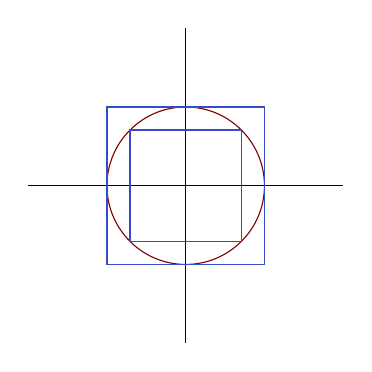
\begin{tikzpicture}
      \draw (-2, 0) -- (2, 0);
      \draw (0, -2) -- (0, 2);
      \draw [mred] circle [radius=1];
      \draw [mblue] (-1, -1) rectangle (1, 1);
      \draw [mblue] (-0.707, -0.707) rectangle (0.707, 0.707);
    \end{tikzpicture}
  \end{center}
  where the blue ones are the balls with respect to $\|\ph \|_\infty$ and the red one is the ball with respect to $\|\ph \|_2$.

  In general, we can consider $\R^n$, again with $\|\ph \|_2$ and $\|\ph \|_\infty$. We have
  \[
    \|\mathbf{x}\|_\infty \leq \|\mathbf{x}\|_2 \leq \sqrt{n}\|\mathbf{x}\|_\infty.
  \]
\end{eg}
These are easy to check manually. However, later we will show that in fact, any two norms on a finite-dimensional vector space are Lipschitz equivalent. Hence it is more interesting to look at infinite dimensional cases.

\begin{eg}
  Let $V = C([0, 1])$ with the norms
  \[
    \|f\|_1 = \int_0^1 |f|\;\d x,\quad \|f\|_\infty = \sup_{[0, 1]}|f|.
  \]
  We clearly have the bound
  \[
    \|f\|_1 \leq \|f\|_\infty.
  \]
  However, there is no constant $b$ such that
  \[
    \|f\| \leq b\|f\|_1
  \]
  for all $f$. This is easy to show by constructing a sequence of functions $f_n$ by
  \begin{center}
    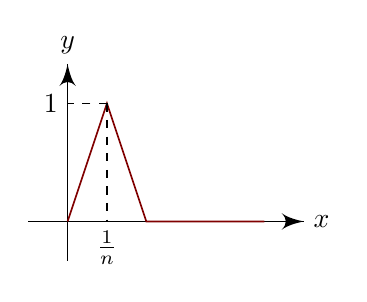
\begin{tikzpicture}
      \draw [->] (-0.5, 0) -- (3, 0) node [right] {$x$};
      \draw [->] (0, -0.5) -- (0, 2) node [above] {$y$};
      \draw [mred, semithick] (0, 0) -- (0.5, 1.5) -- (1, 0) -- (2.5, 0);
      \draw [dashed] (0.5, 1.5) -- +(-0.5, 0) node [left] {$1$};
      \draw [dashed] (0.5, 1.5) -- +(0, -1.5) node [below] {$\frac{1}{n}$};
    \end{tikzpicture}
  \end{center}
  where the width is $\frac{2}{n}$ and the height is $1$. Then $\|f_n\|_\infty = 1$ but $\|f_n\|_1 = \frac{1}{n} \to 0$.
\end{eg}
\begin{eg}
  Similarly, consider the space $\ell^2 = \left\{(x_n): \sum x_n^2 < \infty\right\}$ under the regular $\ell^2$ norm and the $\ell^\infty$ norm. We have
  \[
    \|(x_k)\|_\infty \leq \|(x_k)\|_{\ell^2},
  \]
  but there is no $b$ such that
  \[
    \|(x_k)\|_{\ell^2} \leq b\|(x_k)\|_\infty.
  \]
  For example, we can consider the sequence $x^n = (1, 1, \cdots, 1, 0, 0, \cdots)$, where the first $n$ terms are $1$.
\end{eg}
So far in all our examples, out of the two inequalities, one holds and one does not. Is it possible for both inequalities to not hold? The answer is yes. This is an exercise on the second example sheet as well.

This is all we are going to say about Lipschitz equivalence. We are now going to define convergence, and study the consequences of Lipschitz equivalence to convergence.
\begin{defi}[Bounded subset]
  Let $(V, \|\ph \|)$ be a normed space. A subset $E \subseteq V$ is \emph{bounded} if there is some $R > 0$ such that
  \[
    E \subseteq B_R(\mathbf{0}).
  \]
\end{defi}

\begin{defi}[Convergence of sequence]
  Let $(V, \|\ph\|)$ be a normed space. A sequence $(x_k)$ in $V$ \emph{converges to} $\mathbf{x} \in V$ if $\|\mathbf{x}_k - \mathbf{x}\| \to 0$ (as a sequence in $\R$), ie.
  \[
    (\forall \varepsilon > 0)(\exists N)(\forall k \geq N)\; \|\mathbf{x}_k - \mathbf{x}\| < \varepsilon.
  \]
\end{defi}
These two definitions, obviously, depends on the chosen norm, not just the vector space $V$. However, if two norms are equivalent, then they agree on what is bounded and what converges.
\begin{prop}
  If $\|\ph \|$ and $\|\ph \|'$ are Lipschitz equivalent norms on a vector space $V$, then
  \begin{enumerate}
    \item A subset $E\subseteq V$ is bounded with respect to $\|\ph \|$ if and only if it is bounded with respect to $\|\ph \|'$.
    \item A sequence $x_k$ converges to $x$ with respect to $\|\ph \|$ if and only if it converges to $x$ with respect to $\|\ph \|'$.
  \end{enumerate}
\end{prop}

\begin{proof}\leavevmode
  \begin{enumerate}
    \item This is direct from definition of equivalence.
    \item Say we have $a, b$ such that $a\|\mathbf{y}\| \leq \|\mathbf{y}\|' \leq b\|\mathbf{y}\|$ for all $\mathbf{y}$. So
      \[
        a\|\mathbf{x}_k - \mathbf{x}\| \leq \|\mathbf{x}_k - \mathbf{x}\|' \leq b\|\mathbf{x}_k - \mathbf{x}\|.
      \]
      So $\|\mathbf{x}_k - \mathbf{x}\| \to 0$ if and only if $\|\mathbf{x}_k - \mathbf{x}\|' \to 0$. So done.
  \end{enumerate}
\end{proof}
What if the norms are not equivalent? It is not surprising that there are some sequences that converge with respect to one norm but not another. More surprisingly, it is possible that a sequence converges to different limits under different norms. This is, again, on the second example sheet.

We have some easy facts about convergence:
\begin{prop}
  Let $(V, \|\ph \|)$ be a normed space. Then
  \begin{enumerate}
    \item If $\mathbf{x}_k \to \mathbf{x}$ and $\mathbf{x}_k \to \mathbf{y}$, then $\mathbf{x} = \mathbf{y}$.
    \item If $\mathbf{x}_k \to \mathbf{x}$, then $a\mathbf{x}_k \to a\mathbf{x}$.
    \item If $\mathbf{x}_k \to \mathbf{x}$, $\mathbf{y}_k \to \mathbf{y}$, then $\mathbf{x}_k + \mathbf{y}_k \to \mathbf{x} + \mathbf{y}$.
  \end{enumerate}
\end{prop}

\begin{proof}\leavevmode
  \begin{enumerate}
    \item $\|\mathbf{x} - \mathbf{y}\| \leq \|\mathbf{x} - \mathbf{x}_k\| + \|\mathbf{x}_k - \mathbf{y}\| \to 0$. So $\|\mathbf{x} - \mathbf{y}\| = 0$. So $\mathbf{x} = \mathbf{y}$.
    \item $\|a \mathbf{x}_k - a \mathbf{x}\| = |a|\|\mathbf{x}_k - \mathbf{x}\| \to 0$.
  \item $\|(\mathbf{x}_k + \mathbf{y}_k) - (\mathbf{x} + \mathbf{y})\| \leq \|\mathbf{x}_k - \mathbf{x}\| + \|\mathbf{y}_k - \mathbf{y}\| \to 0$.
  \end{enumerate}
\end{proof}

\begin{prop}
  Convergence in $\R^n$ (with respect to, say, the Euclidean norm) is equivalent to coordinate-wise convergence, ie. $\mathbf{x}^{(k)} \to \mathbf{x}$ if and only if $x^{(k)}_j \to x_j$ for all $j$.
\end{prop}

\begin{proof}
  Fix $\varepsilon > 0$. Suppose $\mathbf{x}^{(k)} \to \mathbf{x}$. Then there is some $N$ such that for any $k \geq N$ such that
  \[
    \|\mathbf{x}^{(k)} - \mathbf{x}\|_2^2 = \sum_{j = 1}^n (x_j^{(k)} - x_j)^2 < \varepsilon.
  \]
  Hence $|x_j^{(k)} - x_j| < \varepsilon$ for all $k \leq N$.

  On the other hand, for any fixed $j$, there is some $N_j$ such that $k \geq N_j$ implies $|x_j^{(k)} - x_j| < \frac{\varepsilon}{\sqrt{n}}$. So if $k \geq \max\{N_j: j = 1, \cdots, n\}$, then
  \[
    \|\mathbf{x}^{(k)} - \mathbf{x}\|_2 = \left(\sum_{j = 1}^n (x_j^{(k)} - x_j)^2\right)^{\frac{1}{2}} < \varepsilon.
  \]
  So done
\end{proof}

Another space we would like to understand is the space of continuous functions. It should be clear that uniform convergence is the same as convergence under the uniform norm, hence the name. However, there is no norm such that convergence under the norm is equivalent to pointwise convergence, ie. pointwise convergence is not normable. In fact, it is not even metrizable. However, we will not prove this.

We'll now generalize the Bolzano-Weierstrass theorem to $\R^n$.
\begin{thm}[Bolzano-Weierstrass theorem in $\R^n$]
  Any bounded sequence in $\R^n$ (with, say, the Euclidean norm) has a convergent subsequence.
\end{thm}

\begin{proof}
  We induct on $n$. The $n = 1$ case is the usual Bolzano-Weierstrass on the real line, which was proved in IA Analysis I.

  Assume the theorem holds in $\R^{n - 1}$, and let $\mathbf{x}^{(k)} = (x^{(k)}_1, \cdots, x_n^{(k)})$ be a bounded sequence in $\R^n$. Then let $\mathbf{y}^{(k)} = (x^{(k)}_1, \cdots, x_{n - 1}^{(k)})$. Since for any $k$, we know that
  \[
    \|\mathbf{y}^{(k)}\|^2 + |x_n^{(k)}|^2 = \|\mathbf{x}^{(k)}\|^2,
  \]
  it follows that both $(\mathbf{y}^{(k)})$ and $(x_n^{(k)})$ are bounded. So by the induction hypothesis, there is a subsequence $(k_j)$ of $(k)$ and some $\mathbf{y} \in \R^{n - 1}$ such that $\mathbf{y}^{(k_j)} \to \mathbf{y}$. Also, by Bolzano-Weierstrass in $\R$, there is a further subsequence $(x_n^{(k_{j_\ell})})$ of $(x_n^{(k_j)})$ that converges to, say, $y_n \in \R$. Then we know that
  \[
    \mathbf{x}^{(k_{j_\ell})} \to (\mathbf{y}, y_n).
  \]
  So done.
\end{proof}

Note that this is generally \emph{not} true for normed spaces. Finite-dimensionality is important for both of these results.

\begin{eg}
  Consider $(\ell^\infty, \|\ph\|_\infty)$. We let $e^{(k)}_j = \delta_{jk}$ be the sequence with $1$ in the $k$th component and $0$ in other components. Then $e_j^{(k)} \to 0$ for all fixed $j$, and hence $e^{(k)}$ converges componentwise to the zero element $0 = (0, 0, \cdots)$. However, $e^{(k)}$ does not converge to the zero element since $\|e^{(k)} - 0\|_\infty = 1$ for all $k$. Also, this is bounded but does not have a convergent subsequence for the same reasons.
\end{eg}

We know that all finite dimensional vector spaces are isomorphic to $\R^n$ as vector spaces for some $n$, and we will later show that all norms on finite dimensional spaces are equivalent. This means every finite-dimensional normed space satisfies the Bolzano-Weierstrass property. Is the converse true? If a normed vector space satisfies the Bolzano-Weierstrass property, must it be finite dimensional? The answer is yes, and the proof is in the example sheet.

\begin{eg}
  Let $C([0, 1])$ have the $\|\ph \|_{L^2}$ norm. Consider $f_n(x) = \sin 2n\pi x$. We know that
  \[
    \|f_n\|^2_{L^2} = \int_0^1 |f_n|^2 = \frac{1}{2}.
  \]
  So it is bounded. However, it doesn't have a convergent subsequence. If it did, say $f_{n_j} \to f$ in $L^2$, then we must have
  \[
    \|f_{n_j} - f_{n_{j + 1}}\|^2 \to 0.
  \]
  However, by direct calculation, we know that
  \[
    \|f_{n_j} - f_{n_{j + 1}}\|^2 = \int_0^1 (\sin sn_j \pi x - \sin 2n_{j + 1}\pi x)^2 = 1.
  \]
\end{eg}
Note that the same argument shows also that the sequence $(\sin 2n\pi x)$ has no subsequence that converges \emph{pointwise} on $[0, 1]$. To see this, we need the result that if $(f_j)$ is a sequence in $C([0, 1])$ that is uniformly bounded with $f_j \to f$ pointwise, then $f_j$ converges to $f$ under the $L^2$ norm. However, we will not be able to prove this (in a nice way) without Lebesgue integration from IID Probability and Measure.

\subsection{Cauchy sequences and completeness}
\begin{defi}[Cauchy sequence]
  Let $(V, \|\ph \|)$ be a normed space. A sequence $(\mathbf{x}^{(k)})$ in $V$ is a \emph{Cauchy sequence} if
  \[
    (\forall \varepsilon)(\exists N)(\forall n, m \geq N)\; \|\mathbf{x}^{(n)} - \mathbf{x}^{(m)}\| < \varepsilon.
  \]
\end{defi}

\begin{defi}[Complete normed space]
  A normed space $(V, \|\ph\|)$ is \emph{complete} if every Cauchy sequence converges to an element in $V$.
\end{defi}

We'll start with some easy facts about Cauchy sequences and complete spaces.
\begin{prop}
  Any convergent sequence is Cauchy.
\end{prop}

\begin{proof}
  If $\mathbf{x}_k \to \mathbf{x}$, then
  \[
    \|\mathbf{x}_k - \mathbf{x}_\ell\| \leq \|\mathbf{x}_k - \mathbf{x}\| + \|\mathbf{x}_\ell - \mathbf{x}\| \to 0 \text{ as }k, \ell \to \infty.
  \]
\end{proof}

\begin{prop}
  A Cauchy sequence is bounded.
\end{prop}

\begin{proof}
  By definition, there is some $N$ such that for all $n \geq N$, we have $\|\mathbf{x}_N - \mathbf{x}_n\| < 1$. So $\|\mathbf{x}_n\| < 1 + \|\mathbf{x}_N\|$ for $n \geq N$. So, for all $n$,
  \[
    \|\mathbf{x}_n\| \leq \max\{\|\mathbf{x}_1\|, \cdots, \|\mathbf{x}_{N - 1}\|, 1 + \|\mathbf{x}_N\|\}.
  \]
\end{proof}

\begin{prop}
  If a Cauchy sequence has a subsequence converging to an element $\mathbf{x}$, then the whole sequence converges to $\mathbf{x}$.
\end{prop}

\begin{proof}
  Suppose $\mathbf{x}_{k_j} \to \mathbf{x}$. Since $(\mathbf{x}_k)$ is Cauchy, given $\varepsilon > 0$, we can choose an $N$ such that $\|\mathbf{x}_n - \mathbf{x}_m\| < \frac{\varepsilon}{2}$ for all $n, m \geq N$. We can also choose $j_0$ such that $k_{j_0} \geq n$ and $\|\mathbf{x}_{k_{j_0}} - \mathbf{x}\| < \frac{\varepsilon}{2}$. Then for any $n \geq N$, we have
  \[
    \|\mathbf{x}_n - \mathbf{x}\| \leq \|\mathbf{x}_n - \mathbf{x}_{k_{j_0}}\| + \|\mathbf{x} - \mathbf{x}_{k_{j_0}}\| < \varepsilon.
  \]
\end{proof}

\begin{prop}
  If $\|\ph \|'$ is Lipschitz equivalent to $\|\ph\|$ on $V$, then $(\mathbf{x}_k)$ is Cauchy with respect to $\|\ph \|$ if and only if $(\mathbf{x}_k)$ is Cauchy with respect to $\|\ph\|'$. Also, $(V, \|\ph\|)$ is complete if and only if $(V, \|\ph\|')$ is complete.
\end{prop}

\begin{proof}
  This follows directly from definition.
\end{proof}

\begin{thm}
  $\R^n$ (with the Euclidean norm, say) is complete.
\end{thm}

\begin{proof}
  The important thing is to know this is true for $n = 1$, which we have proved from Analysis I.

  If $(\mathbf{x}^k)$ is Cauchy in $\R^n$, then $(x_j^{(k)})$ is a Cauchy sequence of real numbers for each $j \in \{1, \cdots, n\}$. By the completeness of the reals, we know that $x_j^k \to x_j \in \R$ for some $x$. So $x^k \to x = (x_1, \cdots, x_n)$ since convergence in $\R^n$ is equivalent to componentwise convergence.
\end{proof}
Note that the spaces $\ell^1, \ell^2, \ell^\infty$ are all complete with respect to the standard norms. Also, $C([0, 1])$ is complete with respect to $\|\ph\|_\infty$, since uniform Cauchy convergence implies uniform convergence, and the uniform limit of continuous functions is continuous. However, $C([0, 1])$ with the $L^1$ or $L^2$ norms are not complete (see example sheet).

The incompleteness of $L^1$ tells us that $C([0, 1])$ is \emph{not large enough} to to be complete under the $L^1$ or $L^2$ norm. In fact, the space of Riemann integrable functions, say $\mathcal{R}([0, 1])$, is the natural space for the $L^1$ norm, and of course contains $C([0, 1])$. As we have previously mentioned, this time $\mathcal{R}([0, 1])$ is \emph{too large} for $\|\ph\|$ to be a norm, since $\int_0^1 |f|\;\d x = 0$ does not imply $f = 0$. This is a problem we can solve. We just have to take the equivalence classes of Riemann integrable functions, where $f$ and $g$ are equivalent if $\int_0^1 |f - g|\;\d x = 0$. But still, $L^1$ is not complete on $\mathcal{R}([0, 1])/{\sim}$. This is a serious problem in the Riemann integral. This eventually lead to the Lebesgue integral, which generalizes the Riemann integral, and gives a complete normed space.

Note that when we quotient our $\mathcal{R}([0, 1])$ by the equivalence relation $f\sim g$ if $\int_0^1 |f - g|\;\d x = 0$, we are not losing too much information about our functions. We know that for the integral to be non-zero, $f - g$ cannot be non-zero at a point of continuity. Hence they agree on all points of continuities. We also know that by Lebesgue's theorem, the set of points of discontinuity has Lebesgue measure zero. So they disagree on at most a set of Lebesgue measure zero.

\begin{eg}
  Let
  \[
    V = \{(x_n) \in \R^\N: x_j = 0\text{ for all but finitely many }j\}.
  \]
  Take the supremum norm $\|\ph\|_\infty$ on $V$. This is a subspace of $\ell^\infty$ (and is sometimes denoted $\ell^0$). Then $(V, \|\ph\|_\infty)$ is \emph{not} complete. We define $x^{(k)} = (1, \frac{1}{2}, \frac{1}{3}, \cdots, \frac{1}{k}, 0, 0, \cdots)$ for $k = 1, 2, 3, \cdots$. Then this is Cauchy, since
  \[
    \|x^{(k)} - x^{(\ell)}\| = \frac{1}{\min\{\ell, k\} + 1} \to 0,
  \]
  but it is not convergent in $V$. If it actually converged to some $x$, then $x^{(k)}_j \to x_j$. So we must have $x_j = \frac{1}{j}$, but this sequence not in $V$.

  We will later show that this is because $V$ is not \emph{closed}, after we define what it means to be closed.
\end{eg}

\begin{defi}[Open set]
  Let $(V, \|\ph\|)$ be a normed space. A subspace $E\subseteq V$ is \emph{open} in $V$ if for any $\mathbf{y} \in E$, there is some $r > 0$ such that
  \[
    B_r(\mathbf{y}) = \{\mathbf{x}\in V: \|\mathbf{x} - \mathbf{y}\| < r\} \subseteq E.
  \]
\end{defi}

We first check that the open ball is open.
\begin{prop}
  $B_r(\mathbf{y})\subseteq V$ is an open subset for all $r > 0$, $\mathbf{y} \in V$.
\end{prop}

\begin{proof}
  Let $\mathbf{x} \in B_r(\mathbf{y})$. Let $\rho = r - \|\mathbf{x} - \mathbf{y}\| > 0$. Then $B_\rho(\mathbf{x}) \subseteq B_r(\mathbf{y})$.
  \begin{center}
    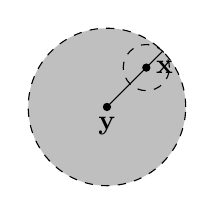
\begin{tikzpicture}
      \draw [dashed, fill=gray!50!white] circle [radius=1];
      \draw (0, 0) -- (0.707, 0.707);
      \draw (0.5, 0.5) node [circ] {} node [right] {$\mathbf{x}$};
      \draw [dashed] (0.5, 0.5) circle [radius=0.293];
      \node [circ] at (0, 0) {};
      \node [below] at (0, 0) {$\mathbf{y}$};
    \end{tikzpicture}
  \end{center}
\end{proof}

\begin{defi}[Limit point]
  Let $(V, \|\ph\|)$ be a normed space, $E\subseteq V$. A point $\mathbf{y} \in V$ is a \emph{limit point} of $E$ if there is a sequence $(\mathbf{x}_k)$ in $E$ with $\mathbf{x}_k \not= \mathbf{y}$ for all $k$ and $\mathbf{x}_k \to \mathbf{y}$.
\end{defi}
(Some people allow $\mathbf{x}_k = \mathbf{y}$, but we will use this definition in this course)

\begin{eg}
  Let $V = \R$, $E = (0, 1)$. Then $0, 1$ are limit points of $E$. The set of \emph{all} limit points is $[0, 1]$.

  If $E' = (0, 1) \cup \{2\}$. Then the set of limit points of $E'$ is still $[0, 1]$.
\end{eg}

There is a nice result characterizing whether a set contains all its limit points.
\begin{prop}
  Let $E\subseteq V$. Then $E$ contains all of its limit points if and only if $V\setminus E$ is open in $V$.
\end{prop}

Using this proposition, we define the following:
\begin{defi}[Closed set]
  Let $(V, \|\ph\|)$ be a normed space. Then $E\subseteq V$ is \emph{closed} if $V\setminus E$ is open, ie. $E$ contains all its limit points.
\end{defi}
Note that sets can be both closed or open; or neither closed nor open.

Before we prove the proposition, we first have a lemma:

\begin{lemma}
  Let $(V, \|\ph\|)$ be a normed space, $E$ any subset of $V$. Then a point $\mathbf{y} \in V$ is a limit point of $E$ if and only if
  \[
    (B_r(\mathbf{y}) \setminus \{\mathbf{y}\}) \cap E \not= \emptyset
  \]
  for every $r$.
\end{lemma}

\begin{proof}
  $(\Rightarrow)$ If $\mathbf{y}$ is a limit point of $E$, then there exists a sequence $(\mathbf{x}_k) \in E$ with $\mathbf{x}_k \not= \mathbf{y}$ for all $k$ and $\mathbf{x}_k \to \mathbf{y}$. Then for every $r$, for sufficiently large $k$, $\mathbf{x}_k \in B_r(\mathbf{y})$. Since $\mathbf{x}_k \not= \{\mathbf{y}\}$ and $\mathbf{x}_k \in E$, the result follows.

  $(\Leftarrow)$ For each $k$, let $r = \frac{1}{k}$. By assumption, we have some $\mathbf{x}_k \in (B_{\frac{1}{k}}(\mathbf{y}) \setminus \{\mathbf{y}\}) \cap E$. Then $\mathbf{x}_k \to \mathbf{y}$, $\mathbf{x}_k \not= \mathbf{y}$ and $\mathbf{x}_k \in E$. So $\mathbf{y}$ is a limit point of $E$.
\end{proof}

Now we can prove our proposition.
\begin{prop}
  Let $E\subseteq V$. Then $E$ contains all of its limit points if and only if $V\setminus E$ is open in $V$.
\end{prop}

\begin{proof}
  $(\Rightarrow)$ Suppose $E$ contains all its limit points. To show $V\setminus E$ is open, we let $\mathbf{y} \in V\setminus E$. So $\mathbf{y}$ is not a limit point of $E$. So for some $r$, we have $(B_r(\mathbf{y})\setminus \{\mathbf{y}\}) \cap E = \emptyset$. Hence it follows that $B_r(\mathbf{y}) \subseteq V\setminus E$ (since $\mathbf{y} \not\in E$).

  $(\Leftarrow)$ Suppose $V\setminus E$ is open. Let $\mathbf{y} \in V\setminus E$. Since $V\setminus E$ is open, there is some $r$ such that $B_r(\mathbf{y}) \subseteq V\setminus E$. By the lemma, $\mathbf{y}$ is not a limit point of $E$. So all limit points of $E$ are in $E$.
\end{proof}

\subsection{Sequential compactness}
In general, there are two different notions of compactness --- ``sequential compactness'' and just ``compactness''. However, in normed spaces (and metric spaces, as we will later encounter), these two notions are equivalent. So we will be lazy and just say ``compactness'' as opposed to ``sequential compactness''.

\begin{defi}[(Sequentially) compact set]
  Let $V$ be a normed vector space. A subset $K\subseteq V$ is said to be \emph{compact} (or \emph{sequentially compact}) if every sequence in $K$ has a subsequence that converges to a point in $K$.
\end{defi}

There are things we can immediately know about the spaces:
\begin{thm}
  Let $(V, \|\ph\|)$ be a normed vector space, $K\subseteq V$ a subset. Then
  \begin{enumerate}
    \item If $K$ is compact, then $K$ is closed and bounded.
    \item If $V$ is $\R^n$ (with, say, the Euclidean norm), then if $K$ is closed and bounded, then $K$ is compact.
  \end{enumerate}
\end{thm}

\begin{proof}\leavevmode
  \begin{enumerate}
    \item Let $K$ be compact. Boundedness is easy: if $K$ is unbounded, then we can generate a sequence $\mathbf{x}_k$ such that $\|\mathbf{x}_k\| \to \infty$. Then this cannot have a convergent subsequence, since any subsequence will also be unbounded, and convergent sequences are bounded. So $K$ must be bounded.

      To show $K$ is closed, let $\mathbf{y}$ be a limit point of $K$. Then there is some $\mathbf{y}_k \in K$ such that $\mathbf{y}_k \to \mathbf{y}$. Then by compactness, there is a subsequence of $\mathbf{y}_k$ converging to some point in $K$. But any subsequence must converge to $\mathbf{y}$. So $\mathbf{y} \in K$.

    \item Let $K$ be closed and bounded. Let $\mathbf{x}_k$ be a sequence in $K$. Since $V = \R^n$ and $K$ is bounded, $(\mathbf{x}_k)$ is a bounded sequence in $\R^n$. So by Bolzano-Weierstrass, this has a convergent subsequence $\mathbf{x}_{k_j}$. By closedness of $V$, we know that the limit is in $K$. So $K$ is compact.
  \end{enumerate}
\end{proof}

\subsection{Mappings between normed spaces}
We are now going to look at functions between normed spaces, and see if they are continuous.

Let $(V, \|\ph\|)$, $(V', \|\ph\|')$ be normed spaces, and let $E \subseteq K$ be a subset, and $f: E \to V'$ a mapping (which is just a function, although we reserve the terminology ``function'' or ``functional'' for when $V' = \R$).

\begin{defi}[Continuity of mapping]
  Let $\mathbf{y} \in E$. We say $f: E \to V'$ is \emph{continuous at} $\mathbf{y}$ if for all $\varepsilon > 0$, there is $\delta > 0$ such that the following holds:
  \[
    (\forall \mathbf{x} \in E)\; \|\mathbf{x} - \mathbf{y}\|_V < \delta \Rightarrow \|f(\mathbf{x}) - f(\mathbf{y})\|_{V'} < \varepsilon.
  \]
\end{defi}
Note that $\mathbf{x} \in E$ and $\|\mathbf{x} - \mathbf{y}\| < \delta$ is equivalent to saying $\mathbf{x} \in B_\delta(\mathbf{y}) \cap E$. Similarly, $\|f(\mathbf{x}) - f(\mathbf{y})\| < \varepsilon$ is equivalent to $f(\mathbf{x}) \in B_\varepsilon(f(\mathbf{y}))$. In other words, $\mathbf{x} \in f^{-1}(B_\varepsilon(f(\mathbf{y})))$. So we can rewrite this statement as there is some $\delta > 0$ such that
\[
  E \cap B_\delta(\mathbf{y}) \subseteq f^{-1}(B_\varepsilon(f(\mathbf{y}))).
\]
We can use this to provide an alternative characterization of continuity.
\begin{thm}
  Let $(V, \|\ph\|)$, $(V', \|\ph\|')$ be normed spaces, $E\subseteq V$, $f: E \to \mathbf{V}'$. Then $f$ is continuous at $\mathbf{y} \in E$ if and only if for any sequence $\mathbf{y}_k \to \mathbf{y}$ in $E$, we have $f(\mathbf{y}_k) \to f(\mathbf{y})$.
\end{thm}

\begin{proof}
  $(\Rightarrow)$ Suppose $f$ is continuous at $\mathbf{y} \in E$, and that $\mathbf{y}_k \to \mathbf{y}$. Given $\varepsilon > 0$, by continuity, there is some $\delta > 0$ such that
  \[
    B_\delta(\mathbf{y}) \cap E \subseteq f^{-1}(B_\varepsilon(f(\mathbf{y}))).
  \]
  For sufficiently large $k$, $\mathbf{y}_k \in B_\delta(\mathbf{y}) \cap E$. So $f(\mathbf{y}_k) \in B_\varepsilon(f(\mathbf{y}))$, or equivalently,
  \[
    |f(\mathbf{y}_k) - f(\mathbf{y})| < \varepsilon.
  \]
  So done.

  $(\Leftarrow)$ If $f$ is not continuous at $y$, then there is some $\varepsilon > 0$ such that for any $k$, we have
  \[
    B_{\frac{1}{k}}(\mathbf{y}) \not\subseteq f^{-1}(B_\varepsilon(f(\mathbf{y}))).
  \]
  Choose $\mathbf{y}_k \in B_{\frac{1}{k}}(\mathbf{y}) \setminus f^{-1}(B_{\varepsilon}(f(\mathbf{y})))$. Then $\mathbf{y}_k \to \mathbf{y}$, $\mathbf{y}_k \in F$, but $\|f(\mathbf{y}_k) - f(\mathbf{y})\| \geq \varepsilon$, contrary to the hypothesis.
\end{proof}

\begin{defi}[Continuous function]
  $f: E \to V'$ is \emph{continuous} if $f$ is continuous at every point $\mathbf{y} \in E$.
\end{defi}

\begin{thm}
  Let $(V, \|\ph\|)$ and $(V', \|\ph\|')$ be normed spaces, and $K$ a compact subset of $V$, and $f: V \to V'$ a continuous function. Then
  \begin{enumerate}
    \item $f(K)$ is compact in $V'$
    \item $f(K)$ is closed and bounded
    \item If $V' = \R$, then the function attains its supremum and infimum, ie. there is some $\mathbf{y}_1, \mathbf{y}_2 \in K$ such that
      \[
        f(\mathbf{y}_1) = \sup\{f(\mathbf{y}): \mathbf{y} \in K\},\quad f(\mathbf{y}_2) = \inf\{f(\mathbf{y}): \mathbf{y} \in K\}.
      \]
  \end{enumerate}
\end{thm}

\begin{proof}\leavevmode
  \begin{enumerate}
    \item Let $(\mathbf{x}_k)$ be a sequence in $f(K)$ with $\mathbf{x}_k = f(\mathbf{y}_k)$ for some $\mathbf{y}_k \in K$. By compactness of $K$, there is a subsequence $(\mathbf{y}_{k_j})$ such that $\mathbf{y}_{k_j} \to \mathbf{y}$. By the previous theorem, we know that $f(\mathbf{y}_{j_k}) \to f(\mathbf{y})$. So $\mathbf{x}_{k_j} \to f(\mathbf{y}) \in f(K)$. So $f(K)$ is compact.
    \item This follows directly from $(i)$, since every compact space is closed and bounded.
    \item If $F$ is any bounded subset of $\R$, then either $\sup F \in F$ or $\sup F$ is a limit point of $F$ (or both), by definition of the supremum. If $F$ is closed and bounded, then any limit point must be in $F$. So $\sup F \in F$. Applying this fact to $F = f(K)$ gives the desired result, and similarly for infimum.
  \end{enumerate}
\end{proof}

Finally, we will end the chapter by proving that any two norms on a finite dimensional space are Lipschitz equivalent. The key lemma is the following:
\begin{lemma}
  Let $V$ be an $n$-dimensional vector space with a basis $\{\mathbf{v}_1, \cdots, \mathbf{v}_n\}$. Then for any $\mathbf{x} \in V$, write $\mathbf{x} = \sum_{j = 1}^n x_j \mathbf{v}_j$, with $x_j \in \R$. We define the Euclidean norm by
  \[
    \|\mathbf{x}\|_2 = \left(\sum x_j^2\right)^{\frac{1}{2}}.
  \]
  Then this is a norm, and $S = \{\mathbf{x} \in V: \|\mathbf{x}\|_2 = 1\}$ is compact in $(V, \|\ph\|_2)$.
\end{lemma}
After we show this, we can easily show that every other norm is equivalent to this norm.

This is not hard to prove, since we know that the unit sphere in $\R^n$ is compact, and we can just pass our things on to $\R^n$.

\begin{proof}
  $\|\ph\|_2$ is well-defined since $x_1, \cdots, x_n$ are uniquely determined by $x$ (by (a certain) definition of basis). It is easy to check that $\|\ph\|_2$ is a norm.

  Given a sequence $\mathbf{x}^{(k)}$ in $S$, if we write $\mathbf{x}^{(k)} = \sum_{j = 1}^n x_j^{(k)} \mathbf{v}_j$. We define the following sequence in $\R^n$:
  \[
    \tilde{\mathbf{x}}^{(k)} = (x_1^{(k)},\cdots, x_n^{(k)}) \in \tilde{S} = \{\tilde{\mathbf{x}} \in \R^n: \|\tilde{\mathbf{x}}\|_{\mathrm{Euclid}} = 1\}.
  \]
  As $\tilde{S}$ is closed and bounded in $\R^n$ under the Euclidean norm, it is compact. Hence there exists a subsequence $\tilde{x}^{(k_j)}$ and $\tilde{x} \in \tilde{S}$ such that $\|\tilde{\mathbf{x}}^{(k_j)} - \tilde{\mathbf{x}} \|_{\mathrm{Euclid}} \to 0$. This says that $\mathbf{x} = \sum_{j = 1}^n x_j \mathbf{v}_j \in S$, and $\|\mathbf{x}^{k_j} - \mathbf{x}\|_2 \to 0$. So done.
\end{proof}

\begin{thm}
  Any two norms on a finite dimensional vector space are Lipschitz equivalent.
\end{thm}

The idea is to pick a basis, and prove that any norm is equivalent to $\|\ph\|_2$.

To show that an arbitrary norm $\|\ph\|$ is equivalent to $\|\ph\|_2$, we have to show that for any $\|\mathbf{x}\|$, we have
\[
  a \|\mathbf{x}\|_2 \leq \|\mathbf{x}\| \leq b\|\mathbf{x}\|_2.
\]
We can divide by $\|\mathbf{x}\|_2$ and obtain an equivalent requirement:
\[
  a \leq \left\|\frac{\mathbf{x}}{\|\mathbf{x}\|_2}\right\| \leq b.
\]
We know that any $\mathbf{x}/\|\mathbf{x}\|_2$ lies in the unit sphere $S = \{\mathbf{x} \in V: \|\mathbf{x}\|_2 = 1\}$. So we want to show that the image of $\|\ph\|$ is bounded. But we know that $S$ is compact. So it suffices to show that $\|\ph\|$ is continuous.
\begin{proof}
  Fix a basis $\{\mathbf{v}_1, \cdots, \mathbf{v}_n\}$ for $V$, and define $\|\ph\|_2$ as in the lemma above. Then $\|\ph\|_2$ is a norm on $V$, and $S = \{\mathbf{x} \in V: \|\mathbf{x}\|_2 = 1\}$, the unit sphere, is compact by above.

  To show that any two norms are equivalent, it suffices to show that if $\|\ph\|$ is any other norm, then it is equivalent to $\|\ph\|_2$, since equivalence is transitive.

  For any
  \[
    \mathbf{x} = \sum_{j = 1}^n x_j \mathbf{v}_j,
  \]
  we have
  \begin{align*}
    \|\mathbf{x}\| &= \left\|\sum_{j = 1}^n x_j \mathbf{v}_j\right\|\\
    &\leq \sum |x_j| \|\mathbf{v}_j\|\\
    &\leq \|\mathbf{x}\|_2 \left(\sum_{j = 1}^n \|\mathbf{v}_j\|^2\right)^{\frac{1}{2}}
  \end{align*}
  by the Cauchy-Schwarz inequality. So $\|\mathbf{x}\| \leq b\|\mathbf{x}\|_2$ for $b = \left(\sum \|\mathbf{v}_j\|^2\right)^{\frac{1}{2}}$.

  To find $a$ such that $\|\mathbf{x}\| \geq a\|\mathbf{x}\|_2$, consider $\|\ph\|: (S, \|\ph\|_2)\to \R$. By above, we know that
  \[
    \|\mathbf{x} - \mathbf{y}\| \leq b \|\mathbf{x} - \mathbf{y}\|_2
  \]
  By the triangle inequality, we know that $\big|\|\mathbf{x}\| - \|\mathbf{y}\|\big| \leq \|\mathbf{x} - \mathbf{y}\|$. So when $\mathbf{x}$ is close to $\mathbf{y}$ under $\|\ph\|_2$, then $\|\mathbf{x}\|$ and $\|\mathbf{y}\|$ are close. So $\|\ph\|: (S, \|\ph\|_2) \to \R$ is continuous. So there is some $\mathbf{x}_0 \in S$ such that $\|\mathbf{x}_0\| = \inf_{x \in S} \|\mathbf{x}\| = a$, say. Since $\|\mathbf{x}_0\| > 0$, we know that $\|\mathbf{x}_0\| > 0$. So $\|\mathbf{x}\| \geq a\|\mathbf{x}\|_2$ for all $\mathbf{x}\in V$.
\end{proof}

The key to the proof is the compactness of the unit sphere of $(V, \|\ph\|)$. On the other hand, compactness of the unit sphere also characterizes finite dimensionality. As you will show in the example sheets, if the unit sphere of a space is compact, then the space must be finite-dimensional.

\begin{cor}
  Let $(V, \|\ph\|)$ be a finite-dimensional normed space.
  \begin{enumerate}
    \item The Bolzano-Weierstrass theorem holds for $V$, ie. any bounded sequence sequence in $V$ has a convergent subsequence.
    \item A subset of $V$ is compact if and only if it is closed and bounded.
  \end{enumerate}
\end{cor}

\begin{proof}
  If a subset is bounded in one norm, then it is bounded in any Lipschitz equivalent norm. Similarly, if it converges to $\mathbf{x}$ in one norm, then it converges to $\mathbf{x}$ in any Lipschitz equivalent norm.

  Since these results hold for the Euclidean norm $\|\ph\|_2$, it follows that they hold for arbitrary finite-dimensional vector spaces.
\end{proof}

\begin{cor}
  Any finite-dimensional normed vector space $(V, \|\ph\|)$ is complete.
\end{cor}

\begin{proof}
  This is true since if a space is complete in one norm, then it is complete in any Lipschitz equivalent norm, and we know that $\R^n$ under the Euclidean norm is complete.
\end{proof}

\section{Metric spaces}
We would like to extend our notions such as convergence, open and closed subsets, compact subsets and continuity from normed spaces to more general sets. Recall that when we defined these notions, we didn't really use the vector space structure of a normed vector space much. Moreover, we mostly defined these things in terms of convergence of sequences. For example, a space is closed if it contains all its limits, and a space is open if its complement is closed.

So what do we actually need in order to define convergence, and hence all the notions we've been using? Recall we define $\mathbf{x}_k \to \mathbf{x}$ to mean $\|\mathbf{x}_k - \mathbf{x}\| \to 0$ as a sequence in $\R$. What is $\|\mathbf{x}_k - \mathbf{x}\|$ really about? It is measuring the distance between $\mathbf{x}_k$ and $\mathbf{x}$. So what we really need is a measure of distance.

To do so, we can define a distance function $d: V\times V \to \R$ by $d(x, y) = \|x - y\|$. Then we can define $x_k \to x$ to mean $d(x_k, x) \to 0$.

Hence, given \emph{any} function $d: V\times V \to \R$, we can define a notion of ``convergence'' as above. However, we want this to be well-behaved. In particular, we would want the limits of sequences to be unique, and any constant sequence $x_k = x$ should converge to $x$.

We will come up with some restrictions on what $d$ can be based on these requirements.

We can look at our proof of uniqueness of limits (for normed spaces), and see what properties of $d$ we used. Recall that to prove the uniqueness of limits, we first assume that $x_k \to x$ and $x_k \to y$. Then we noticed
\[
  \|x - y\| \leq \|x - x_k\| + \|x_k - y\| \to 0,
\]
and hence $\|x - y\| = 0$. So $x = y$. We can reformulate this argument in terms of $d$. We first start with
\[
  d(x, y) \leq d(x, x_k) + d(x_k, y).
\]
To obtain this equation, we are relying on the triangle inequality. So we would want $d$ to satisfy the triangle inequality

After obtaining this, we know that $d(x_k, y) \to 0$, since this is just the definition of convergence. However, we do not immediately know $d(x, x_k) \to 0$, since we are given a fact about $d(x_k, x)$, not $d(x, x_k)$. Hence we need the property that $d(x_k, x) = d(x, x_k)$. This is symmetry.

Combining this, we know that
\[
  d(x, y) \leq 0.
\]
From this, we want to say that in fact, $d(x, y) = 0$, and thus $x = y$. Hence we need the property that $d(x, y) \geq 0$ for all $x, y$, and that $d(x, y) = 0$ implies $x = y$.

Finally, to show that a constant sequence has a limit, suppose $x_k = x$ for all $k \in \N$. Then we know that $d(x, x_k) = d(x, x)$ should tend to $0$. So we must have $d(x, x) = 0$ for all $x$.

We will use these properties to define \emph{metric spaces}.
\subsection{Preliminary definitions}
\begin{defi}[Metric space]
  Let $X$ be any set. A \emph{metric} on $X$ is a function $d: X\times X \to \R$ that satisfies
  \begin{itemize}
    \item $d(x, y) \geq 0$ with equality iff $x = y$\hfill(non-negativity)
    \item $d(x, y) = d(y, x)$\hfill(symmetry)
    \item $d(x, y) \leq d(x, z) + d(z, y)$\hfill(triangle inequality)
  \end{itemize}
  The pair $(X, d)$ is called a \emph{metric space}.
\end{defi}
We have seen that we can define convergence in terms of a metric. Hence, we can also define open subsets, closed subsets, compact spaces, continuous functions etc. for metric spaces, in a manner consistent with what we had for normed spaces. Moreover, we will show that many of our theorems for normed spaces are also valid in metric spaces.

\begin{eg}\leavevmode
  \begin{enumerate}
    \item $\R^n$ with the Euclidean \emph{metric} is a metric space, where the metric is defined by
      \[
        d(x, y) = \|x - y\| = \sqrt{\sum (x_j - y_j)^2}.
      \]
    \item More generally, if $(V, \|\ph\|)$ is a normed space, then $d(x, y) = \|x - y\|$ defines a metric on $V$.
    \item Discrete metric: let $X$ be any set, and define
      \[
        d(x, y) =
        \begin{cases}
          0 & x = y\\
          1 & x\not= y
        \end{cases}.
      \]
    \item Given a metric space $(X, d)$, we define
      \[
        g(x, y) = \min\{1, d(x, y)\}.
      \]
      Then this is a metric on $X$. Similarly, if we define
      \[
        h(x, y) = \frac{d(x, y)}{1 + d(x, y)}
      \]
      is also a metric on $X$. In both cases, we obtain a \emph{bounded} metric.

      The axioms are easily shown to be satisfied, apart from the triangle inequality. So let's check the triangle inequality for $h$. We'll use a general fact that for numbers $a, c \geq 0, b, d > 0$ we have
      \[
        \frac{a}{b} \leq \frac{c}{d} \Leftrightarrow \frac{a}{a + b} \leq \frac{c}{c + d}.
      \]
      Based on this fact, we can start with
      \[
        d(x, y) \leq d(x, z) + d(z, y).
      \]
      Then we obtain
      \begin{align*}
        \frac{d(x, y)}{1 + d(x, y)} &\leq \frac{d(x, z) + d(z, y)}{1 + d(x, z) + d(z, y)} \\
        &= \frac{d(x, z)}{1 + d(x, z) + d(z, y)} + \frac{d(z, y)}{1 + d(x, z) + d(z, y)} \\
        &\leq \frac{d(x, z)}{1 + d(x, z)} + \frac{d(z, y)}{1 + d(z, y)}.
      \end{align*}
      So done.
  \end{enumerate}
\end{eg}

We can also extend the notion of Lipschitz equivalence to metric spaces.
\begin{defi}[Lipschitz equivalent metrics]
  Metrics $d, d'$ on a set $X$ are said to be \emph{Lipschitz equivalent} if there are (positive) constants $A, B$ such that
  \[
    A d(x, y) \leq d'(x, y) \leq B d(x, y)
  \]
  for all $x, y \in X$.
\end{defi}
Clearly, any Lipschitz equivalent norms give Lipschitz equivalent metrics. Any metric coming from a norm in $\R^n$ is thus Lipschitz equivalent to the Euclidean metric. We will later show that two equivalent norms induce the same \emph{topology}. In some sense, Lipschitz equivalent norms are indistinguishable.

\begin{defi}[Metric subspace]
  Given a metric space $(X, d)$ and a subset $Y\subseteq X$, the restriction $d|_{Y \times Y} \to \R$ is a metric on $Y$. This is called the \emph{induced metric} or \emph{subspace metric}.
\end{defi}
Note that unlike vector subspaces, we do not require our subsets to have any structure. We can take \emph{any} subset of $X$ and get a metric subspace.

\begin{eg}
  Any subspace of $\R^n$ is a metric space with the Euclidean metric.
\end{eg}

\begin{defi}[Convergence]
  Let $(X, d)$ be a metric space. A sequence $x_n \in X$ is said to \emph{converge} to $x$ if $d(x_n, x) \to 0$ as a real sequence. In other words,
  \[
    (\forall \varepsilon)(\exists K)(\forall k > K)\, d(x_k, x) < \varepsilon.
  \]
  Alternatively, this says that given any $\varepsilon$, for sufficiently large $k$, we get $x_k \in B_\varepsilon(x)$.
\end{defi}
Again, $B_r(a)$ is the open ball centered at $a$ with radius $r$, defined as
\[
  B_r(a) = \{x \in X: d(x, a) < r\}.
\]
\begin{prop}
  The limit of a convergent sequence is unique.
\end{prop}

\begin{proof}
  Same as that of normed spaces.
\end{proof}
Note that notions such as convergence, open and closed subsets and continuity of mappings all make sense in an even more general setting called \emph{topological spaces}. However, in this setting, limits of convergent sequences can fail to be unique. We will not worry ourselves about these since we will just focus on metric spaces.

\subsection{Topology of metric spaces}
We will define open subsets of a metric space in exactly the same way as we did for normed spaces.
\begin{defi}[Open subset]
  Let $(X, d)$ be a metric space. A subset $U\subseteq X$ is \emph{open} if for every $y \in U$, there is some $r > 0$ such that $B_r(y) \subseteq U$.
\end{defi}
This means we can write any open $U$ as a union of open balls:
\[
  U = \bigcup_{y \in U} B_{r(y)} (y)
\]
for appropriate choices of $r(y)$ for every $y$.

It is easy to check that every open ball $B_r(y)$ is an open set. The proof is exactly the same as what we had for normed spaces.

Note that two different metrics $d, d'$ on the same set $X$ may give rise to the same collection of open subsets.
\begin{eg}
  Lipschitz equivalent metrics give rise to the same collection of open sets, ie. if $d, d'$ are Lipschitz equivalent, then a subset $U \subseteq X$ is open with respect to $d$ if and only if it is open with respect to $d'$. Proof is left as an easy exercise.
\end{eg}
The converse, however, is not necessarily true.
\begin{eg}
  Let $X = \R$, $d(x, y) = |x - y|$ and $d'(x, y) = \min\{1, |x - y|\}$. It is easy to check that these are not Lipschitz equivalent, but they induce the same set collection of open subsets.
\end{eg}

\begin{defi}[Topology]
  Let $(X, d)$ be a metric space. The \emph{topology} on $(X, d)$ is the collection of open subsets of $X$. We say it is the topology induced by the metric.
\end{defi}

\begin{defi}[Topological notion]
  A notion or property is said to be a \emph{topological} notion or property if it only depends on the topology, and not the metric.
\end{defi}

We will introduce a useful terminology before we go on:

\begin{defi}[Neighbourhood]
  Given a metric space $X$ and a point $x \in X$, a \emph{neighbourhood} of $x$ is an open set containing $x$.
\end{defi}
Some people do not require the set to be open. Instead, it requires a neighbourhood to be a set that contains an open subset that contains $x$, but this is too complicated, and we could as well work with open subsets directly.

Clearly, being a neighbourhood is a topological property.

\begin{prop}
  Let $(X, d)$ be a metric space. Then $x_k \to x$ if and only if for every neighbourhood $V$ of $x$, there exists some $K$ such that $x_k \in V$ for all $k \geq K$. Hence convergence is a topological notion.
\end{prop}

\begin{proof}
  $(\Rightarrow)$ Suppose $x_k \to X$, and let $V$ be any neighbourhood of $x$. Since $V$ is open, by definition, there exists some $\varepsilon$ such that $B_\varepsilon(x) \subseteq V$. By definition of convergence, there is some $K$ such that $x_k \in B_\varepsilon(x)$ for $k \geq K$. So $x_k \in V$ whenever $k \geq K$.

  $(\Rightarrow)$ Since every open ball is a neighbourhood, this direction follows directly from definition.
\end{proof}

\begin{thm}
  Let $(X, d)$ be a metric space. Then
  \begin{enumerate}
    \item The union of \emph{any} collection of open sets is open
    \item The intersection of finitely many open sets is open.
    \item $\emptyset$ and $X$ are open.
  \end{enumerate}
\end{thm}

\begin{proof}\leavevmode
  \begin{enumerate}
    \item Let $U = \bigcup_\alpha V_\alpha$, where each $V_\alpha$ is open. If $x\in U$, then $x\in V_\alpha$ for some $\alpha$. Since $V_\alpha$ is open, there exists $\delta > 0$ such that $B_\delta(x) \subseteq V_\alpha$. So $B_\delta (x) \subseteq \bigcup_\alpha V_\alpha = U$. So $U$ is open.
    \item Let $U = \bigcap_{i = 1}^n V_\alpha$, where each $V_\alpha$ is open. If $x\in V$, then $x\in V_i$ for all $i = 1, \cdots, n$. So $\exists \delta_i > 0$ with $B_{\delta_i}(x) \subseteq V_i$. Take $\delta = \min\{\delta_1, \cdots, \delta_n\}$. So $B_\delta(x) \subseteq V_i$ for all $i$. So $B_\delta(x) \subseteq V$. So $V$ is open.
    \item $\emptyset$ satisfies the definition of an open subset vacuously. $X$ is open since for any $x$, $B_1(x) \subseteq X$.
  \end{enumerate}
\end{proof}
This theorem is not important in this course. However, this will be a key defining property we will use when we define topological spaces in IB Metric and Topological Spaces.

We can now define closed subsets and characterize them using open subsets, in exactly the same way as for normed spaces.
\begin{defi}[Limit point]
  Let $(X, d)$ be a metric space and $E\subseteq X$. A point $y \in X$ is a \emph{limit point} of $E$ if there exists a sequence $x_k \in E$, $x_k \not= y$ such that $x_k \to y$.
\end{defi}

\begin{defi}[Closed subset]
  A subset $E\subseteq X$ is \emph{closed} if $E$ contains all its limit points.
\end{defi}

\begin{prop}
  A subset is closed if and only if its complement is open.
\end{prop}

\begin{proof}
  Exactly the same as that of normed spaces. It is useful to observe that $y \in X$ is a limit point of $E$ if and only if $(B_r(y)\setminus \{y\}) \cap E \not= \emptyset$ for all $r > 0$.
\end{proof}

We can write down an analogous theorem for closed sets:
\begin{thm}
  Let $(X, d)$ be a metric space. Then
  \begin{enumerate}
    \item The intersection of \emph{any} collection of closed sets is closed
    \item The union of finitely many closed sets is closed.
    \item $\emptyset$ and $X$ are closed.
  \end{enumerate}
\end{thm}

\begin{proof}
  By taking complements of the result for open subsets.
\end{proof}

\begin{prop}
  Let $(X, d)$ be a metric space and $x \in X$. Then the singleton $\{x\}$ is a closed subset, and hence any finite subset is closed.
\end{prop}

\begin{proof}
  Let $y \in X \setminus \{x\}$. So $d(x, y) > 0$. Then $B_{d(y, x)}(x) \subseteq X\setminus \{x\}$. So $X\setminus \{x\}$ is open. So $\{x\}$ is closed.

  Alternatively, since $\{x\}$ has no limit points, it contains all its limit points. So it is closed.
\end{proof}

\subsection{Cauchy sequences and completeness}

\begin{defi}[Cauchy sequence]
  Let $(X, d)$ be a metric space. A sequence $(x_n)$ in $X$ is \emph{Cauchy} if
  \[
    (\forall \varepsilon)(\exists N)(\forall n, m, m \geq N)\; d(x_n, x_m) < \varepsilon.
  \]
\end{defi}

\begin{prop}
  Let $(X, d)$ be a metric space. Then
  \begin{enumerate}
    \item Any convergent sequence is Cauchy.
    \item If a Cauchy sequence has a convergent subsequence, then the original sequence converges to the same limit.
  \end{enumerate}
\end{prop}

\begin{proof}\leavevmode
  \begin{enumerate}
    \item If $x_k \to x$, then
      \[
        d(x_m, x_n) \leq d(x_m, x) + d(x_n, x) \to 0
      \]
      as $m, n \to \infty$.
    \item Suppose $x_{k_j} \to x$. Since $(x_k)$ is Cauchy, given $\varepsilon > 0$, we can choose an $N$ such that $d(x_n, x_m) < \frac{\varepsilon}{2}$ for all $n, m \geq N$. We can also choose $j_0$ such that $k_{j_0} \geq n$ and $d(x_{k_{j_0}}, x) < \frac{\varepsilon}{2}$. Then for any $n \geq N$, we have
      \[
        d(x_n, x) \leq d(x_n, x_{k_{j_0}}) + d(x, x_{k_{j_0}}) < \varepsilon.
      \]
  \end{enumerate}
\end{proof}

\begin{defi}[Complete metric space]
  A metric space is complete if all Cauchy sequences converge.
\end{defi}

\begin{eg}
  Let $X = \R^n$ with the Euclidean metric. Then $X$ is complete.
\end{eg}
It is easy to produce incomplete metric spaces. Since arbitrary subsets of metric spaces are subspaces, we can just remove some random elements to make it incomplete.

\begin{eg}
  Let $X = (0, 1) \subseteq \R$ with the Euclidean metric. Then this is incomplete, since $\left(\frac{1}{k}\right)$ is Cauchy but has no limit in $X$.

  Similarly, $X = \R \setminus \{0\}$ is incomplete. Note, however, that it is possible to construct a metric $d'$ on $X = \R \setminus \{0\}$ such that $d'$ induces the same topology on $X$, but makes $X$ complete. This shows that completeness is not a topological property. The actual construction is left as an exercise on the example sheet.
\end{eg}

\begin{eg}
  We can create an easy example of an incomplete metric on $\R^n$. We start by defining $h: \R^n \to \R^n$ by
  \[
    h(x) = \frac{x}{1 + \|x\|},
  \]
  where $\|\ph\|$ is the Euclidean norm. We can check that this is injective: if $h(x) = h(y)$, taking the norm gives
  \[
    \frac{\|x\|}{1 + \|x\|} = \frac{\|y\|}{ 1 + \|y\|}.
  \]
  So we must have $\|x\| = \|y\|$, ie. $x = y$. So $h(x) = h(y)$ implies $x = y$.

  Now we define
  \[
    d(x, y) = \|h(x) - h(y)\|.
  \]
  It is an easy check that this is a metric on $\R^n$.

  In fact, we can show that $h: \R^n \to B_1(0)$, and $h$ is a homeomorphism (ie. continuous bijection with continuous inverse) between $\R^n$ and the unit ball $B_1(0)$, both with the Euclidean metric.

  To show that this metric is incomplete, we can consider the sequence $x_k = (k - 1) e_1$, where $e_1 = (1, 0, 0, \cdots, 0)$ is the usual basis vector. Then $(x_k)$ is Cauchy in $(\R^n, d)$. To show this, first note that
  \[
    h(x_k) = \left(1 - \frac{1}{k}\right) e_1.
  \]
  Hence we have
  \[
    d(x_n, x_m) = \|h(x_n) - h(x_m)\| = \left|\frac{1}{n} - \frac{1}{m}\right| \to 0.
  \]
  So it is Cauchy. To show it does not converge in $(\R^n, d)$, suppose $d(x_k, x) \to 0$ for some $x$. Then since
  \[
    d(x_k, x) = \|h(x_k) - h(x)\| \geq \big| \|h(x_k)\| - \|h(x)\|\big|,
  \]
  We must have
  \[
    \|h(x)\| = \lim_{k \to \infty} \|h(x_k)\| = 1.
  \]
  However, there is no element with $\|h(x)\| = 1$.
\end{eg}
What is happening in this example, is that we are pulling in the whole $\R^n$ in to the unit ball. Then under this norm, a sequence that ``goes to infinity'' in the usual norm will be Cauchy in this norm, but we have nothing at infinity for it to converge to.

Suppose we have a complete metric space $(X, d)$. We know that we can form arbitrary subspaces by taking subsets of $X$. When will this be complete? Clearly it has to be closed, since it has to include all its limit points. It turns it closedness is a sufficient condition.
\begin{thm}
  Let $(X, d)$ be a metric space, $Y \subseteq X$ any subset. Then
  \begin{enumerate}
    \item If $(Y, d|_{Y\times Y})$ is complete, then $Y$ is closed in $X$.
    \item If $(X, d)$ is complete, then $(Y, d|_{Y\times Y})$ is complete if and only if it is closed.
  \end{enumerate}
\end{thm}

\begin{proof}\leavevmode
  \begin{enumerate}
    \item Let $x \in X$ be a limit point of $Y$. Then there is some sequence $x_k \to x$, where each $x_k \in Y$. Since $(x_k)$ is convergent, it is a Cauchy sequence. Hence it is Cauchy in $Y$. By completeness of $Y$, $(x_k)$ has to converge to some point in $Y$. By uniqueness of limits, this limit must be $x$. So $x \in Y$. So $Y$ contains all its limit points.
    \item We have just showed that if $Y$ is complete, then it is closed. Now suppose $Y$ is closed. Let $(x_k)$ be a Cauchy sequence in $Y$. Then $(x_k)$ is Cauchy in $X$. Since $X$ is complete, $x_k\to x$ for some $x \in X$. Since $x$ is a limit point of $Y$, we must have $x \in Y$. So $x_k$ converges in $Y$.
  \end{enumerate}
\end{proof}

\subsection{Compactness}
\begin{defi}[(Sequential) compactness]
  A metric space $(X, d)$ is \emph{(sequentially) compact} if every sequence in $X$ has a convergent subsequence.

  A subset $K\subseteq X$ is said to be compact if $(K, d|_{K\times K})$ is compact. In other words, $K$ is compact if every sequence in $K$ has a subsequence that converges to some point in $K$.
\end{defi}
Note that when we say every sequence has a convergent subsequence, we do not require it to be bounded. This is unlike the statement of the Bolzano-Weierstrass theorem. In particular, $\R$ is \emph{not} compact.

It follows from definition that compactness is a topological property, since it is defined in terms of convergence, and convergence is defined in terms of open sets.

The following theorem relates completeness with compactness.
\begin{thm}
  All compact spaces are complete and bounded.
\end{thm}
Note that $X$ is bounded iff $X = B_r(x_0)$ for some $r \in \R, x_0 \in X$ (or $X$ is empty).

\begin{proof}
  Let $(X, d)$ be a compact metric space. Let $(x_k)$ be Cauchy in $X$. By compactness, it has some convergent subsequence, say $x_{k_j} \to x$. So $x_k \to x$. So it is complete.

  If $(X, d)$ is not bounded, by definition, for any $x_0$, there is a sequence $(x_k)$ such that $d(x_k, x_0) > k$ for every $k$. But then $(x_k)$ cannot have a convergent subsequence. Otherwise, if $x_{k_j} \to x$, then
  \[
    d(x_{k_j}, x_0) \leq d(x_{k_j}, x) + d(x, x_0)
  \]
  and is bounded, which is a contradiction.
\end{proof}
This implies that if $(X, d)$ is a metric space and $E\subseteq X$, and $E$ is compact, then $E$ is bounded, ie. $E \subseteq B_R(x_0)$ for some $x_0 \in X, R > 0$, and $E$ with the subspace metric is complete. Hence $E$ is closed as a subset of $X$.

The converse is not true. For example, recall if we have an infinite-dimensional normed vector space, then the closed unit sphere is complete and bounded, but not compact. Alternatively, we can take $X = \R$ with the metric $d(x, y) = \min\{1, |x - y|\}$. This is clearly bounded (by $1$), and it is easy to check that this is complete. However, this is not compact since the sequence $x_k = k$ has no convergent subsequence.

However, we can strengthen the condition of boundedness to \emph{total} boundedness, and get the equivalence between ``completeness and total boundedness'' and compactness.

\begin{defi}[Totally bounded*]
  A metric space $(X, d)$ is said to be \emph{totally bounded} if for all $\varepsilon > 0$, there is an integer $N \in \N$ and points $x_1, \cdots, x_N \in X$ such that
  \[
    X = \bigcup_{i = 1}^N B_\varepsilon (x_i).
  \]
\end{defi}
It is easy to check that being totally bounded implies being bounded. We then have the following strengthening of the previous theorem.
\begin{thm}(non-examinable)
  Let $(X, d)$ be a metric space. Then $X$ is compact if and only if $X$ is complete and totally bounded.
\end{thm}

\begin{proof}
  $(\Leftarrow)$ Let $X$ be complete and totally bounded, $(y_i) \in X$. For every $j \in \N$, there exists a finite set of points $E_j$ such that every point is within $\frac{1}{j}$ of one of these points.

  Now since $E_1$ is finite, there is some $x_1 \in E_1$ such that there are infinitely many $y_i$'s in $B(x_1, 1)$. Pick the first $y_i$ in $B(x_1, 1)$ and call it $y_{i_1}$.

  Now there is some $x_2 \in E_2$ such that there are infinitely many $y_i$'s in $B(x_1, 1) \cap B(x_2, \frac{1}{2})$. Pick the one with smallest value of $i > i_1$, and call this $y_{i_2}$. Continue till infinity.

  This procedure gives a sequence $x_i \in E_i$ and subsequence $(y_{i_k})$, and also
  \[
    y_{i_n} \in \bigcap_{j = 1}^n B\left(x_j, \frac{1}{j}\right).
  \]
  It is easy to see that $(y_{i_n})$ is Cauchy since if $m > n$, then $d(y_{i_m}, y_{i_n}) < \frac{2}{n}$. By completeness of $X$, this subsequence converges.

  $(\Rightarrow)$ Compactness implying completeness is proved above. Suppose $X$ is not totally bounded. We show it is not compact by constructing a sequence with no Cauchy subsequence.

  Suppose $\varepsilon$ is such that there is no finite set of points $x_1, \cdots, x_N$ with
  \[
    X = \bigcup_{i = 1}^N B_\varepsilon (x_i).
  \]
  We will construct our sequence iteratively.

  Start by picking an arbitrary $y_1$. Pick $y_2$ such that $d(y_1, y_2) \geq \varepsilon$. This exists or else $B_\varepsilon(y_1)$ covers all of $X$.

  Now given $y_1, \cdots, y_n$ such that $d(y_i, y_j) \geq \varepsilon$ for all $i, j = 1, \cdots, n$, $i \not= j$, we pick $y_{n + 1}$ such that $d(y_{n + 1}, y_j) \geq \varepsilon$ for all $j = 1, \cdots, n$. Again, this exists, or else $\bigcup_{i = 1}^n B_\varepsilon(y_i)$ covers $X$. Then clearly the sequence $(y_n)$ is not Cauchy. So done.
\end{proof}
In IID Linear Analysis, we will prove the Arzel\`a-Ascoli theorem that characterizes the compact subsets of the space $C([a. b])$ in a very concrete way, which is in some sense a strengthening of this result.

\subsection{Continuous functions}
We are going to look at continuous mappings between metric spaces.
\begin{defi}[Continuity]
  Let $(X, d)$ and $(X', d')$ be metric spaces. A function $f: X \to X'$ is \emph{continuous at $y \in X$} if
  \[
    (\forall \varepsilon > 0)(\exists \delta > 0)(\forall x)\; d(x, y) < \delta \Rightarrow d'(f(x), f(y)) < \varepsilon.
  \]
  This is true if and only if for every $\varepsilon > 0$, there is some $\delta > 0$ such that
  \[
    B_\delta(y) \subseteq f^{-1}B_\varepsilon(f(x)).
  \]
  $f$ is \emph{continuous} if $f$ is continuous at each $y \in X$.
\end{defi}

\begin{defi}[Uniform continuity]
  $f$ is \emph{uniformly continuous} on $X$ if
  \[
    (\forall \varepsilon > 0)(\exists \delta > 0)(\forall x, y \in X)\; d(x, y) < \delta \Rightarrow d(f(x), f(y)) < \varepsilon.
  \]
  This is true if and only if for all $\varepsilon$, there is some $\delta$ such that for \emph{all} $y$, we have
  \[
    B_\delta(y) \subseteq f^{-1} (B_\varepsilon(f(y))).
  \]
\end{defi}

\begin{defi}[Lipschitz function and Lipschitz constant]
  $f$ is said to be \emph{Lipschitz} on $X$ if there is some $K \in [0, \infty)$ such that for all $x, y \in X$,
  \[
    d'(f(x), f(y)) \leq K d(x, y)
  \]
  \emph{Any} such $K$ is called a Lipschitz constant.
\end{defi}
It is easy to show
\[
  \text{Lipschitz} \Rightarrow \text{uniform continuity} \Rightarrow \text{continuity}.
\]
We have seen many examples that continuity does not imply uniform continuity. To show that uniform continuity does not imply Lipschitz, take $X = X' = \R$. We define the metrics as
\[
  d(x, y) = \min\{1, |x - y|\}, \quad d'(x, y) = |x - y|.
\]
Now consider the function $f: (X, d) \to (X', d')$ defined by $f(x) = x$. We can then check that this is uniformly continuous but not Lipschitz.

Note that the statement that metrics $d$ and $d'$ are Lipschitz equivalent is equivalent to saying the two identity maps $i: (X, d) \to (X, d')$ and $i': (X, d') \to (X, d)$ are Lipschitz, hence the name.

Note also that the metric \emph{itself} is also a Lipschitz map for any metric. Here we are viewing the metric as a function $d: X\times X \to \R$, with the metric on $X\times X$ defined as
\[
  \tilde{d}((x_1, y_1), (x_2, y_2)) = d(x_1, x_2) + d(y_1, y_2).
\]
This is a consequence of the triangle inequality, since
\[
  d(x_1, y_1) \leq d(x_1, x_2) + d(x_2, y_2) + d(y_1, y_2).
\]
Moving the middle term to the left gives
\[
  d(x_1, y_1) - d(x_2, y_2) \leq \tilde{d}((x_1, y_1), (x_2, y_2))
\]
Swapping the theorems around, we can put in the absolute value to obtain
\[
  |d(x_1, y_1) - d(x_2, y_2)| \leq \tilde{d}((x_1, y_1), (x_2, y_2))
\]
Recall that at the very beginning, we proved that a continuous map from a closed, bounded interval is automatically uniformly continuous. This is true whenever the domain is compact.
\begin{thm}
  Let $(X, d)$ be a compact metric space, and $(X', d')$ is any metric space. If $f: X\to X'$ be continuous, then $f$ is uniformly continuous.
\end{thm}

This is exactly the same proof as what we had for the $[0, 1]$ case.
\begin{proof}
  We are going to prove by contradiction. Suppose $f: X \to X'$ is not uniformly continuous. Since $f$ is not uniformly continuous, there is some $\varepsilon > 0$ such that for all $\delta = \frac{1}{n}$, there is some $x_n, y_n$ such that $d(x_n, y_n) < \frac{1}{n}$ but $d'(f(x_n), f(y_n)) > \varepsilon$.

  By compactness of $X$, $(x_n)$ has a convergent subsequence $(x_{n_i}) \to x$. Then we also have $y_{n_i}\to x$. So by continuity, we must have $f(x_{n_i}) \to f(x)$ and $f(y_{n_i}) \to f(x)$. But $d'(f(x_{n_i}), f(y_{n_i})) > \varepsilon$ for all $n_i$. This is a contradiction.
\end{proof}

In the proof, we have secretly used (part of) the following characterization of continuity:
\begin{thm}
  Let $(X, d)$ and $(X', d')$ be metric spaces, and $f: X\to X'$. Then the following are equivalent:
  \begin{enumerate}
    \item $f$ is continuous at $y$.
    \item $f(x_k) \to f(y)$ for every sequence $(x_k)$ in $X$ with $x_k \to y$.
    \item For every neighbourhood $V$ of $f(y)$, there is a neighbourhood $U$ of $y$ such that $U\subseteq f^{-1}(V)$.
  \end{enumerate}
\end{thm}
Note that the definition of continuity says something like (iii), but with open balls instead of open sets. So this should not be surprising.

\begin{proof}\leavevmode
  \begin{itemize}
    \item (i) $\Leftrightarrow$ (ii): The argument for this is the same as for normed spaces.
    \item (i) $\Rightarrow$ (iii): Let $V$ be a neighbourhood of $f(y)$. Then by definition there is $\varepsilon > 0$ such that $B_\varepsilon (f(y)) \subseteq V$. By continuity of $f$, there is some $\delta$ such that
      \[
        B_\delta(y) \subseteq f^{-1}(B_\varepsilon(f(y))) \subseteq f^{-1}(V).
      \]
      Set $U = B_\varepsilon(y)$ and done.
    \item (iii) $\Rightarrow$ (i): for any $\varepsilon$, use the hypothesis with $V = B_\varepsilon (f(y))$ to get a neighbourhood $U$ of $y$ such that
      \[
        U \subseteq f^{-1}(V) = f^{-1}(B_{\varepsilon}(f(y))).
      \]
      Since $U$ is open, there is some $\delta$ such that $B_\delta(y) \subseteq U$. So we get
      \[
        B_\delta(y) \subseteq f^{-1}(B_\varepsilon(f(y))).
      \]
      So we get continuity.
  \end{itemize}
\end{proof}

\begin{cor}
  A function $f: (X, d) \to (X', d')$ is continuous if $f^{-1}(V)$ is open in $X$ whenever $V$ is open in $X'$.
\end{cor}

\begin{proof}
  Follows directly from the equivalence of (i) and (iii) in the theorem above.
\end{proof}

\subsection{The contraction mapping theorem}
If you have already taken IB Metric and Topological Spaces, then you were probably bored by the above sections, since you've already met them all. Finally, we get to something new. This section is comprised of just two theorems. The first is the contraction mapping theorem, and we will use it to prove Picard-Lindel\"of existence theorem. Later, we will prove the inverse function theorem using the contraction mapping theorem. All of these are really powerful and important theorems in analysis. They have many more applications and useful corollaries, but we do not have time to get into those.

\begin{defi}[Contraction mapping]
  Let $(X, d)$ be metric space. A mapping $f: X \to X$ is a \emph{contraction} if there exists some $\lambda$ with $0 \leq \lambda < 1$ such that
  \[
    d(f(x), f(y)) \leq \lambda d(x, y).
  \]
\end{defi}
Note that a contraction mapping is by definition Lipschitz and hence (uniformly) continuous.

\begin{thm}[Contraction mapping theorem]
  Let $X$ be a (non-empty) complete metric space, and if $f: X \to X$ is a contraction, then $f$ has a \emph{unique} fixed point, ie. there is a unique $x$ such that $f(x) = x$.

  Moreover, if $f: X\to X$ is a function such that $f^{(m)}: X\to X$ (ie. $f$ composed with itself $m$ times) is a contraction for some $m$, then $f$ has a unique fixed point.
\end{thm}
We can see finding fixed points as the process of solving equations. One important application we will have is to use this to solve \emph{differential} equations.

Note that the theorem is false if we drop the completeness assumption. For example, $f: (0, 1) \to (0, 1)$ defined by $\frac{x}{2}$ is clearly a contraction with no fixed point. The theorem is also false if we drop the assumption $\lambda < 1$. In fact, it is not enough to assume $d(f(x), f(y)) < d(x, y)$ for all $x, y$. A counterexample is to be found on example sheet 3.

\begin{proof}
  We first focus on the case where $f$ itself is a contraction.

  Uniqueness is straightforward. By assumption, there is some $0 \leq \lambda < 1$ such that
  \[
     d(f(x), f(y)) \leq \lambda d(x, y)
  \]
  for all $x, y \in X$. If $x$ and $y$ are both fixed points, then this says
  \[
    d(x, y) = d(f(x), f(y)) \leq \lambda d(x, y).
  \]
  This is possible only if $d(x, y) = 0$, ie. $x = y$.

  To prove existence, the idea is to pick a point $x_0$ and keep applying $f$. Let $x_0 \in X$. We define the sequence $(x_n)$ inductively by
  \[
    x_{n + 1} = f(x_n).
  \]
  We first show that this is Cauchy. For any $n \geq 1$, we can compute
  \[
    d(x_{n + 1}, x_n) = d(f(x_n), f(x_{n - 1})) \leq \lambda d(x_n, x_{n - 1}) \leq \lambda^n d(x_1, x_0).
  \]
  Since this is true for any $n$, for $m > n$, we have
  \begin{align*}
    d(x_m, x_n) &\leq d(x_m, x_{m - 1}) + d(x_{m - 1}, x_{m - 2}) + \cdots + d(x_{n + 1}, x_n) \\
    &= \sum_{j = n}^{m - 1} d(x_{j + 1}, x_j)\\
    &= \sum_{j = n}^{m - 1} \lambda^j d(x_1, x_0)\\
    &\leq d(x_1, x_0) \sum_{j = n}^\infty \lambda^j\\
    &= \frac{\lambda^n}{1 - \lambda} d(x_1, x_0).
  \end{align*}
  Note that we have again used the property that $\lambda < 1$.

  This implies $d(x_m, x_n) \to 0$ as $m, n \to \infty$. So this sequence is Cauchy. By the completeness of $X$, there exists some $x \in X$ such that $x_n \to x$. Since $f$ is a contraction, it is continuous. So $f(x_n) \to f(x)$. However, by definition $f(x_n) = x_{n + 1}$. So taking the limit on both sides, we get $f(x) = x$. So $x$ is a fixed point.

  Now suppose that $f^{(m)}$ is a contraction for some $m$. Hence by the first part, there is a unique $x \in X$ such that $f^{(m)}(x) = x$. But then
  \[
    f^{(m)}(f(x)) = f^{(m + 1)}(x) = f(f^{(m)}(x)) = f(x).
  \]
  So $f(x)$ is also a fixed point of $f^{(n)}(x)$. By uniqueness of fixed points, we must have $f(x) = x$. Since any fixed point of $f$ is clearly a fixed point of $f^{(n)}$ as well, it follows that $x$ is the unique fixed point of $f$.
\end{proof}

Based on the proof of the theorem, we have the following error estimate in the contraction mapping theorem: for $x_0 \in X$ and $x_n = f(x_{n - 1})$, we showed that for $m > n$, we have
\[
  d(x_m, x_n) \leq \frac{\lambda^n}{1 - \lambda}d(x_1, x_0).
\]
If $x_n \to x$, taking the limit of the above bound as $m \to \infty$ gives
\[
  d(x, x_n) \leq \frac{\lambda^n}{1 - \lambda} d(x_1, x_0).
\]
This is valid for all $n$.

We are now going to use this to obtain the Picard-Lindel\"of existence theorem for ordinary differential equations. The objective is as follows. Suppose we are given a function
\[
  \mathbf{F} = (F_1, F_2, \cdots, F_n): \R\times \R^n \to \R^n.
\]
We interpret the $\R$ as time and the $\R^n$ as space.

Given $t_0 \in \R$ and $\mathbf{x}_0 \in \R^n$, we want to know when can we find a solution to the ODE
\[
  \frac{\d \mathbf{f}}{\d t} = \mathbf{F}(t, \mathbf{f}(t))
\]
subject to $f(t_0) = \mathbf{x}_0$. We would like this solution to be valid (at least) for all $t$ in some interval $I$ containing $t_0$.

More explicitly, we want to understand when will there be some $\varepsilon > 0$ and a differentiable function $\mathbf{f} = (f_1, \cdots, f_n): (t_0 - \varepsilon, t_0 + \varepsilon) \to \R^n$ (ie. $f_j: (t_0 - \varepsilon, t_0 + \varepsilon) \to \R$ is differentiable for all $j$) satisfying
\[
  \frac{\d f_j}{\d t} = F_j(t, f_1(t), \cdots, f_n(t))
\]
such that $f_j(t_0) = x_0^{(j)}$ for all $j = 1, \ldots, n$ and $t \in (t_0 - \varepsilon, t_0 + \varepsilon)$.

We can imagine this scenario as a particle moving in $\R^n$, passing through $\mathbf{x}_0$ at time $t_0$. We then ask if there is a trajectory $\mathbf{f}(t)$ such that the velocity of the particle at any time $t$ is given by $\mathbf{F}(t, \mathbf{f}(t))$.

This is a complicated system, since it is a coupled system of many variables. Explicit solutions are usually impossible, but we in certain cases, we can prove the existence of a solution. Of course, solutions need not exist for arbitrary $F$. For example, there will be no solution if $F$ is everywhere discontinuous, since any derivative is continuous in a dense set of points. The Picard-Lindel\"of existence theorem gives us sufficient conditions for a unique solution to exists.

We will need the following notation
\begin{notation}
  For $\mathbf{x}_0 \in \R^n$, $R > 0$, we let
  \[
    \overline{B_R(\mathbf{x}_0)} = \{\mathbf{x} \in \R^n: \|\mathbf{x} - \mathbf{x}_0\|_2 \leq R\}.
  \]
\end{notation}
Then the theorem says
\begin{thm}[Picard-Lindel\"of existence theorem]
  Let $\mathbf{x}_0 \in \R^n$, $R > 0$, $a < b$, $t_0 \in [a, b]$. Let $\mathbf{F}: [a, b] \times \overline{B_R(\mathbf{x}_0)} \to \R^n$ be a continuous function satisfying
  \[
    \|\mathbf{F}(t, \mathbf{x}) - \mathbf{F}(t, \mathbf{y})\|_2 \leq \kappa\|\mathbf{x} - \mathbf{y}\|_2
  \]
  for some fixed $\kappa > 0$ and all $t \in [a, b], \mathbf{x} \in \overline{B_R(\mathbf{x}_0)}$. In other words, $F(t, \ph): \R^n \to \R^n$ is Lipschitz on $\overline{B_R(\mathbf{x}_0})$ with the same Lipschitz constant for every $t$. Then
  \begin{enumerate}
    \item There exists an $\varepsilon > 0$ and a unique differentiable function $f: [t_0 - \varepsilon, t_0 + \varepsilon] \cap [a, b] \to \R^n$ such that
      \[
        \frac{\d \mathbf{f}}{\d t} = \mathbf{F}(t, \mathbf{f}(t))\tag{$*$}
      \]
      and $\mathbf{f}(t_0) = \mathbf{x}_0$.
    \item If
      \[
        \sup_{[a, b] \times \overline{B_R(\mathbf{x}_0)}} \|\mathbf{F}\|_2 \leq \frac{R}{b - a},
      \]
      then there exists a unique differential function $f: [a, b] \to \R$ that satisfies the differential equation and boundary conditions above.
  \end{enumerate}
\end{thm}
Even $n = 1$ is an important, special, non-trivial case. Even if we have only one dimension, explicit solutions may be very difficult to find, if not impossible. For example,
\[
  \frac{\d f}{\d t} = f^2 + \sin f + e^f
\]
would be almost impossible to solve. However, the theorem tells us there will be a solution, at least locally.

Note that any differentiable $f$ satisfying the differential equation is automatically continuously differentiable, since the derivative is $\mathbf{F}(t, \mathbf{f}(t))$, which is continuous.

Before we prove the theorem, we first show the requirements are indeed necessary. We first look at that $\varepsilon$ in (i). Without the addition requirement in (ii), there might not exist a solution globally on $[a, b]$. For example, we can consider the $n = 1$ case, where we want to solve
\[
  \frac{\d f}{\d t} = f^2,
\]
with boundary condition $f(0) = 1$. Our $F(t, f) = f^2$ is a nice, uniformly Lipschitz function on any $[0, \times b] \times B_R(1) = [0, b] \times [1 - R, 1 + R]$. However, we will shortly see that there is no global solution.

If we assume $f \not= 0$, then for all $t \in [0, b]$, the equation is equivalent to
\[
  \frac{\d}{\d t}(t + f^{-1}) = 0.
\]
So we need $t + f^{-1}$ to be constant. The initial conditions tells us this constant is $1$. So we have
\[
  f(t) = \frac{1}{1 - t}.
\]
Hence the solution on $[0, 1)$ is $\frac{1}{1 - t}$. Any solution on $[0, b]$ must agree with this on $[0, 1)$. So if $b \geq 1$, then there is no solution in $[0, b]$.

The Lipschitz condition is also necessary to guarantee uniqueness. Without this condition, existence of a solution is still guaranteed (but is another theorem, the Cauchy-Peano theorem), but we could have many different solutions. For example, we can consider the differential equation
\[
  \frac{\d f}{\d t} = \sqrt{|f|}
\]
with $f(0) = 0$. Here $F(t, x) = \sqrt{|x|}$ is not Lipschitz near $x = 0$. It is easy to see that both $f = 0$ and $f(t) = \frac{1}{4}t^2$ are both solutions. In fact, for any $\alpha \in [0, b]$, the function
\[
  f_\alpha(t) =
  \begin{cases}
    0 & 0 \leq t \leq \alpha\\
    \frac{1}{4}(t - \alpha)^2 & \alpha \leq t \leq b
  \end{cases}
\]
is also a solution. So we have an infinite number of solutions.

We are now going to use the contraction mapping theorem to prove this. In general, this is a very useful idea. It is in fact possible to use other fixed point theorems to show the existence of solutions to partial differential equations. This is \emph{much} more difficult, but has many far-reaching important applications to theoretical physics and geometry, say. For these, see Part III courses.

\begin{proof}
  First, note that (ii) implies (i). We know that
  \[
    \sup_{[a, b]\times \overline{B_R(\mathbf{x})}}\|\mathbf{F}\|
  \]
  is bounded since it is a continuous function on a compact domain. So we can pick an $\varepsilon$ such that
  \[
    2\varepsilon \leq \frac{R}{\sup_{[a, b]\times \overline{B_R(\mathbf{x})}}\|\mathbf{F}\|}.
  \]
  Then writing $[t_0 - \varepsilon, t_0 + \varepsilon] \cap [a, b] = [a_1, b_1]$, we have
  \[
    \sup_{[a_1, b_1]\times \overline{B_R(\mathbf{x})}}\|\mathbf{F}\| \leq \sup_{[a, b]\times \overline{B_R(\mathbf{x})}}\|\mathbf{F}\| \leq \frac{R}{2\varepsilon} \leq \frac{R}{b_1 - a_1}.
  \]
  So (ii) implies there is a solution on $[t_0 - \varepsilon, t_0 + \varepsilon] \cap [a, b]$. Hence it suffices to prove (ii).

  To apply the contraction mapping theorem, we need to convert this into a fixed point problem. The key is to reformulate the problem as an integral equation. We know that a differentiable $\mathbf{f}: [a, b] \to \R^n$ satisfies the differential equation $(*)$ if and only if $\mathbf{f}: [a, b] \to \overline{B_R(\mathbf{x}_0)}$ is continuous and satisfies
  \[
    \mathbf{f}(t) = \mathbf{x}_0 + \int_{t_0}^t \mathbf{F}(s, \mathbf{f}(s))\;\d s
  \]
  by the fundamental theorem of calculus. Note that we don't require $f$ is differentiable, since if a continuous $f$ satisfies this equation, it is automatically differentiable by the fundamental theorem of calculus. This is very helpful, since we can work over the much larger vector space of continuous functions, and it would be easier to find a solution.

  We let $X = C([a, b], \overline{B_R(\mathbf{x}_0)})$. We equip $X$ with the supremum metric
  \[
    \|\mathbf{g} - \mathbf{h}\| = \sup_{t \in [a, b]} \|\mathbf{g}(t) - \mathbf{h}(t)\|_2.
  \]
  We see that $X$ is a closed subset of the complete metric space $C([a, b] , \R^n)$ (again taken with the supremum metric). So $X$ is complete. For every $\mathbf{g} \in X$, we define a function $T\mathbf{g}: [a, b] \to \R^n$ by
  \[
    (T\mathbf{g}) (t) = \mathbf{x}_0 + \int_{t_0}^t \mathbf{F}(s, \mathbf{g}(s))\;\d s.
  \]
  Our differential equation is thus
  \[
    \mathbf{f} = T\mathbf{f}.
  \]
  So we first want to show that $T$ is actually mapping $X \to X$, ie. $T\mathbf{g} \in X$ whenever $\mathbf{g} \in X$, and the prove it is a contraction map.

  We have
  \begin{align*}
    \|T\mathbf{g}(t) - \mathbf{x}_0\|_2 &= \left\|\int_{t_0}^t \mathbf{F}(s, \mathbf{g}(s))\;\d s\right\|\\
    &\leq \left|\int_{t_0}^t \|\mathbf{F} (s, \mathbf{g}(s))\|_2\;\d s\right|\\
    &\leq \sup_{[a, b] \times \overline{B_R(\mathbf{x}_0)}} \|\mathbf{F}\| \cdot |b - a|\\
    &\leq R
  \end{align*}
  Hence we know that $T\mathbf{g}(t) \in \overline{B}_R(\mathbf{x}_0)$. So $T \mathbf{g} \in X$.

  Next, we need to show this is a contraction. However, it turns out $T$ need not be a contraction. Instead, what we have is that for $\mathbf{g}_1, \mathbf{g}_2 \in X$, we have
  \begin{align*}
    \|T \mathbf{g}_1(t) - T\mathbf{g}_2(t)\|_2 &= \left\|\int_{t_0}^t \mathbf{F}(s, \mathbf{g}_1(s)) - \mathbf{F}(s, \mathbf{g}_2(s))\;\d s\right\|_2\\
    &\leq \left|\int_{t_0}^t \|\mathbf{F}(s, \mathbf{g}_1(s)) - \mathbf{F}(s, \mathbf{g}_2(s))\|_2 \;\d s \right|\\
    &\leq \kappa (b - a) \|\mathbf{g}_1 - \mathbf{g}_2\|_\infty
  \end{align*}
  by the Lipschitz condition on $F$. If we indeed have
  \[
    \kappa (b - a) < 1 \tag{$\dagger$},
  \]
  then the contraction mapping theorem gives an $f \in X$ such that
  \[
    T\mathbf{f} = \mathbf{f},
  \]
  ie.
  \[
    \mathbf{f} = \mathbf{x}_0 + \int_{t_0}^t \mathbf{F}(s, \mathbf{f}(s))\;\d s.
  \]
  However, we do not necessarily have $(\dagger)$. There are many ways we can solve this problem. Here, we can solve it by finding an $m$ such that $T^{(m)} = T\circ T \circ \cdots \circ T: X \to X$ is a contraction map. We will in fact show that this map satisfies the bound
  \[
    \sup_{t \in [a, b]} \|T^{(m)}\mathbf{g}_1(t) - T^{(m)}\mathbf{g}_2(t)\| \leq \frac{(b - a)^m \kappa^m}{m!} \sup_{t \in [a, b]} \|\mathbf{g}_1(t) - \mathbf{g}_2(t)\|. \tag{$\ddag$}
  \]
  The key is the $m!$, since this grows much faster than any exponential. Given this bound, we know that for sufficiently large $m$, we have
  \[
    \frac{(b - a)^m \kappa^m}{m!} < 1,
  \]
  ie. $T^{(m)}$ is a contraction. So by the contraction mapping theorem, the result holds.

  So it only remains to prove the bound. To prove this, we prove instead the pointwise bound: for any $t \in [a, b]$, we have
  \[
    \|T^{(m)}\mathbf{g}_1(t) - T^{(m)}\mathbf{g}_2(t)\|_2 \leq \frac{(|t - t_0|)^m \kappa^m}{m!} \sup_{s \in [t_0, t]}\|\mathbf{g}_1(s) - \mathbf{g}_2(s)\|.
  \]
  From this, taking the supremum on the left, we obtain the bound $(\ddag)$.

  To prove this pointwise bound, we induct on $m$. We wlog assume $t > t_0$. We know that for every $m$, the difference is given by
  \begin{align*}
    \|T^{(m)}g_1(t) - T^{(m)}g_2(t)\|_2 &= \left\|\int_{t_0}^t F(s, T^{(m - 1)}g_1(s)) - F(s, T^{(m - 1)} g_2(s))\;\d s\right\|_2.\\
    &\leq \kappa\int_{t_0}^t \|T^{(m - 1)} g_1(s) - T^{(m - 1)} g_2(s)\|_2 \;\d s.
  \end{align*}
  This is true for all $m$. If $m = 1$, then this gives
  \[
    \|T g_1(t) - T g_2(t)\| \leq k(t - t_0) \sup_{[t_0, t]} \|g_1 - g_2\|_2.
  \]
  So the base case is done.

  For $m \geq 2$, assume by induction the bound holds with $m - 1$ in place of $m$. Then the bounds give
  \begin{align*}
    \| T^{(m)} g_1(t) - T^{(m)} g_2(t)\| &\leq k \int_{t_0}^t \frac{k^{m - 1}(s - t_0)^{m - 1}}{(m - 1)!} \sup_{[t_0, s]} \|g_1 - g_2\|_2 \;\d s\\
    &\leq \frac{k^m}{(m - 1)!} \sup_{[t_0, t]} \|g_1 - g_2\|_2 \int_{t_0}^t (s - t_0)^{m - 1} \;\d s\\
    &= \frac{k^m (t - t_0)^m}{m!} \sup_{[t_0, t]} \|g_1 - g_2\|_2.
  \end{align*}
  So done.
\end{proof}
Note that to get the factor of $m!$, we had to actually perform the integral, instead of just bounding $(s - t_0)^{m -1 }$ by $(t - t_0)$. In general, this is a good strategy if we want tight bounds. Instead of bounding
\[
  \left|\int_a^b f(x) \;\d x\right| \leq (b - a) \sup |f(x)|,
\]
we write $f(x) = g(x) h(x)$, where $h(x)$ is something easily integrable. Then we can have a bound
\[
  \left|\int_a^b f(x) \;\d x\right| \leq \sup |g(x)| \int_a^b |h(x)| \;\d x.
\]

\section{Differentiation from \texorpdfstring{$\R^m$}{Rm} to \texorpdfstring{$\R^n$}{Rn}}
\subsection{Differentiation from \texorpdfstring{$\R^m$}{Rm} to \texorpdfstring{$\R^n$}{Rn}}
We are now going to investigate differentiation of functions $f: \R^n \to \R^m$. The hard part is to first come up with a sensible definition of what this means. There is no obvious way to generalize what we had for real functions. After defining it, we will need to do some hard work to come up with easy ways to check if functions are differentiable. Then we can use it to prove some useful results like the mean value inequality. We will always use the usual Euclidean norm.


To define differentiation in $\R^n$, we first we need a definition of the limit.

\begin{defi}[Limit of function]
  Let $E \subseteq \R^n$ and $f: E \to \R^m$. Let $\mathbf{a}\in \R^n$ be a limit point of $E$, and let $\mathbf{b} \in \R^m$. We say
  \[
    \lim_{\mathbf{x} \to \mathbf{a}} f(\mathbf{x}) = \mathbf{b}
  \]
  if for every $\varepsilon > 0$, there is some $\delta > 0$ such that
  \[
    (\forall \mathbf{x} \in E)\; 0 < \|\mathbf{x} - \mathbf{a}\| < \delta \Rightarrow \|f(\mathbf{x}) - \mathbf{b}\| < \varepsilon.
  \]
\end{defi}
As in the case of $\R$ in IA Analysis I, we do not impose any requirements on $F$ when $\mathbf{x} = \mathbf{a}$. In particular, we don't assume that $a$ is in the domain $E$.

We would like a definition of differentiation for functions $f: \R^n \to \R$ (or more generally $\mathbf{f}: \R^n \to \R^m$) that directly extends the familiar definition on the real line. Recall that if $f: (b, c) \to \R$ and $a \in (b, c)$, we say $f$ is \emph{differentiable} if the limit
\[
  Df(a) = f'(a) = \lim_{h \to 0} \frac{f(a + h) - f(a)}{h}\tag{$*$}
\]
exists (as a real number). This cannot be extended to higher dimensions directly, since $\mathbf{h}$ would become a vector in $\R^n$, and it is not clear what we mean by dividing by a vector. We might try dividing by $\|\mathbf{h}\|$ instead, ie. require that
\[
  \lim_{\mathbf{h}\to \mathbf{0}}\frac{f(\mathbf{a} + \mathbf{h}) - f(\mathbf{a})}{\|\mathbf{h}\|}
\]
exists. However, this is clearly wrong, since in the case of $n = 1$, this reduces to the existence of the limit
\[
  \frac{f(a + h) - f(a)}{|h|},
\]
which almost never exists, eg. when $f(x) = x$. It is also possible that this exists while the genuine derivative does not, eg. when $f(x) = |x|$, at $x = 0$. So this is clearly wrong.

Now we are a bit stuck. We need to divide by something, and that thing better be a scalar. $\|\mathbf{h}\|$ is not exactly what we want. What should we do? The idea is move $f'(a)$ to the other side of the equation, and $(*)$ becomes
\[
  \lim_{h \to 0} \frac{f(a + h) - f(a) - f'(a) h}{h} = 0.
\]
Now if we replace $h$ by $|h|$, nothing changes. So this is equivalent to
\[
  \lim_{h \to 0} \frac{f(a + h) - f(a) - f'(a) h}{|h|} = 0.
\]
In other words, the function $f$ is differentiable if there is some $A$ such that
\[
  \lim_{h \to 0} \frac{f(a + h) - f(a) - A h}{|h|} = 0,
\]
and we call $A$ the derivative.

We are now in a good shape to generalize. Note that if $f: \R^n \to \R$ is a real-valued function, then $f(a + h) - f(a)$ is a scalar, but $h$ is a vector. So $A$ is not just a number, but a (row) vector. In general, if our function $\mathbf{f}: \R^n \to \R^m$ is vector-valued, then our $A$ should be an $m \times n$ matrix. Alternatively, $A$ is a linear map from $\R^n$ to $\R^m$.

\begin{defi}[Differentiation in $\R^n$]
  Let $U\subseteq \R^n$ be open, $\mathbf{f}: \R^n \to \R^m$. We say $\mathbf{f}$ is differentiable at a point $\mathbf{a} \in U$ if there exists a linear map $A: \R^n \to \R^m$ such that
  \[
    \lim_{\mathbf{h} \to \mathbf{0}} \frac{\mathbf{f}(\mathbf{a} + \mathbf{h}) - \mathbf{f}(\mathbf{a}) - A \mathbf{h}}{\|\mathbf{h}\|} = 0.
  \]
  We call $A$ the \emph{derivative of $\mathbf{f}$ at $a$}. We write the derivative as $D \mathbf{f}(\mathbf{a})$.
\end{defi}
This is equivalent to saying
\[
  \lim_{\mathbf{x} \to \mathbf{a}} \frac{\mathbf{f}(\mathbf{x}) - \mathbf{f}(\mathbf{a}) - A (\mathbf{x} - \mathbf{a})}{\|\mathbf{x} - \mathbf{a}\|} = 0.
\]
Note that this is completely consistent with our usual definition the case where $n = m = 1$, as we have discussed above, since a linear transformation $\alpha: \R \to \R$ is just given by $\alpha(h) = Ah$ for some real $A \in \R$.

One might instead attempt to define differentiability as follows: for any $f: \R^m \to \R$, we say $f$ is differentiable at $x$ if $f$ is differentiable when restricted to any line passing through $x$. However, this is a weaker notion, and we will later see that if we define differentiability this way, then differentiability will no longer imply continuity, which is bad.

Having defined differentiation, we want to show that the derivative is unique.
\begin{prop}[Uniqueness of derivative]
  Derivatives are unique.
\end{prop}

\begin{proof}
  Suppose $A, B: \R^n \to \R^m$ both satisfy the condition
  \begin{align*}
    \lim_{\mathbf{h} \to \mathbf{0}} \frac{\mathbf{f}(\mathbf{a} + \mathbf{h}) - \mathbf{f}(\mathbf{a}) - A \mathbf{h}}{\|\mathbf{h}\|} &= \mathbf{0}\\
    \lim_{\mathbf{h} \to \mathbf{0}} \frac{\mathbf{f}(\mathbf{a} + \mathbf{h}) - \mathbf{f}(\mathbf{a}) - B \mathbf{h}}{\|\mathbf{h}\|} &= \mathbf{0}.
  \end{align*}
  By the triangle inequality, we get
  \[
    \|(B - A) \mathbf{h}\| \leq \|\mathbf{f}(\mathbf{a} + \mathbf{h}) - f(\mathbf{a}) - A\mathbf{h}\| + \|f(\mathbf{a} + \mathbf{h}) - f(\mathbf{a}) - B\mathbf{h}\|.
  \]
  So
  \[
    \frac{\|(B - A)\mathbf{h}\|}{\|\mathbf{h}\|} \to 0
  \]
  as $h \to 0$. We set $\mathbf{h} = t\mathbf{u}$ in this proof to get
  \[
    \frac{\|(B - A) t\mathbf{u}\|}{\|t\mathbf{u}\|} \to 0
  \]
  as $t \to \infty$. Since $(B - A)$ is linear, we know
  \[
    \frac{\|(B - A) t\mathbf{u}\|}{\|t\mathbf{u}\|} = \frac{\|(B - A) \mathbf{u}\|}{\|\mathbf{u}\|}.
  \]
  So $(B - A) \mathbf{u} = \mathbf{0}$ for all $\mathbf{u} \in \R^n$. So $B = A$.
\end{proof}

\begin{notation}
  We write $L(\R^n; \R^m)$ for the space of linear maps $A: \R^n \to \R^m$.
\end{notation}
So $D\mathbf{f}(\mathbf{a}) \in L(\R^n; \R^m)$.

To avoid having to write limits and divisions all over the place, we have the following convenient notation:
\begin{notation}[Little $o$ notation]
  For any function $\alpha: B_r(0) \subseteq \R^n \to \R^m$, write
  \[
    \alpha(\mathbf{h}) = o(\mathbf{h})
  \]
  if
  \[
    \frac{\alpha(\mathbf{h})}{\|\mathbf{h}\|} \to 0\text{ as }\mathbf{h}\to \mathbf{0}.
  \]
  In other words, $\alpha\to \mathbf{0}$ faster than $\|\mathbf{h}\|$ as $\mathbf{h}\to \mathbf{0}$.

  Note that officially, $\alpha(\mathbf{h}) = o(\mathbf{h})$ as a whole is a piece of notation, and does not represent equality.
\end{notation}
Then the condition for differentiability can be written as: $f: U \to \R^m$ is differentiable at $\mathbf{a} \in U$ if there is some $A$ with
\[
  f(\mathbf{a} + \mathbf{h}) - f(\mathbf{a}) - A\mathbf{h} = o(\mathbf{h}).
\]
Alternatively,
\[
  f(\mathbf{a} + \mathbf{h}) = f(\mathbf{a}) + A\mathbf{h} + o(\mathbf{h}).
\]
Note that we require the domain $U$ of $\mathbf{f}$ to be open, so that for each $\mathbf{a} \in U$, there is a small ball around $\mathbf{a}$ on which $\mathbf{f}$ is defined, so $\mathbf{f}(\mathbf{a} + \mathbf{h})$ is defined for for sufficiently small $\mathbf{h}$. We could relax this condition and consider ``one-sided'' derivatives instead, but we will not look into these in this course.

We can interpret the definition of differentiability as saying we can find a ``good'' linear approximation (technically, it is affine, not linear) to the function $\mathbf{f}$ near $\mathbf{a}$.

While the definition of the derivative is good, it is purely existential. This is unlike the definition of differentiability of real functions, where we are asked to compute an explicit limit --- if the limit exists, that's the derivative. If not, it is not differentiable. In the higher-dimensional world, this is not the cases. We have completely no idea where to find the derivative, even if we know it exists. So we would like an explicit formula for it.

The idea is to look at specific ``directions'' instead of finding the general derivative. As always, let $\mathbf{f}: U \to \R^m$ be differentiable at $\mathbf{a} \in U$. Fix some $\mathbf{u} \in \R^n$, take $\mathbf{h} = t \mathbf{u}$ (with $t \in \R$). Assuming $\mathbf{u} \not= \mathbf{0}$, differentiability tells
\[
  \lim_{t \to 0} \frac{\mathbf{f}(\mathbf{a} + t\mathbf{u}) - \mathbf{f}(\mathbf{a}) - D \mathbf{f}(\mathbf{a}) (t\mathbf{u})}{\|t \mathbf{u}\|} = 0.
\]
This is equivalent to saying
\[
  \lim_{t \to 0} \frac{\mathbf{f}(\mathbf{a} + t\mathbf{u}) - \mathbf{f}(\mathbf{a}) - t D \mathbf{f}(\mathbf{a}) \mathbf{u}}{|t|\|\mathbf{u}\|} = 0.
\]
Since $\|\mathbf{u}\|$ is fixed, This in turn is equivalent to
\[
  \lim_{t \to 0} \frac{\mathbf{f}(\mathbf{a} + t\mathbf{u}) - \mathbf{f}(\mathbf{a}) - t D \mathbf{f}(\mathbf{a}) \mathbf{u}}{t} = 0.
\]
This, finally, is equal to
\[
  D\mathbf{f}(\mathbf{a}) \mathbf{u} = \lim_{t \to 0} \frac{\mathbf{f}(\mathbf{a} + t\mathbf{u}) - \mathbf{f}(\mathbf{a})}{t}.
\]
We derived this assuming $\mathbf{u} \not= \mathbf{0}$, but this is trivially true for $\mathbf{u} = \mathbf{0}$. So this valid for all $\mathbf{u}$.

This is of the same form as the usual derivative, and it is usually not too difficult to compute this limit. Note, however, that this says if the derivative exists, then the limit above is related to the derivative as above. However, even if the limit exists for all $\mathbf{u}$, we still cannot conclude that the derivative exists.

Regardless, even if the derivative does not exist, this limit is still often a useful notion.

\begin{defi}[Directional derivative]
  We write
  \[
    D_{\mathbf{u}} \mathbf{f}(\mathbf{a}) = \lim_{t\to 0} \frac{\mathbf{f}(\mathbf{a} + t\mathbf{u}) - \mathbf{f}(\mathbf{a})}{t}
  \]
  whenever this limit exists. We call $D_{\mathbf{u}} \mathbf{f} (\mathbf{a})$ the \emph{directional derivative} of $\mathbf{f}$ at $\mathbf{a} \in U$ in the direction of $\mathbf{u} \in \R^n$.

  By definition, we have
  \[
    D_{\mathbf{u}} \mathbf{f}(\mathbf{a}) = \left.\frac{\d}{\d t}\right|_{t = 0} \mathbf{f}(\mathbf{a} + t\mathbf{u}).
  \]
\end{defi}

Often, it is convenient to focus on the special cases where $\mathbf{u} = \mathbf{e}_j$, a member of the standard basis for $\R^n$. This is known as the \emph{partial derivative}. By convention, this is defined for real-valued functions only, but the same definition works for any $\R^m$-valued function.

\begin{defi}[Partial derivative]
  The \emph{$j$th partial derivative} of $f: U \to \R$ at $\mathbf{a} \in U$ is
  \[
    D_{\mathbf{e}_j} f(\mathbf{a}) = \lim_{t \to \infty} \frac{f(\mathbf{a} + t \mathbf{e}_j) - f(\mathbf{a})}{t},
  \]
  when the limit exists. We often write this as
  \[
    D_{\mathbf{e}_j} f(\mathbf{a}) = D_j f(\mathbf{a}) = \frac{\partial f}{\partial x_j}.
  \]
\end{defi}
Note that these definitions do not require differentiability of $\mathbf{f}$ at $\mathbf{a}$. We will see some examples shortly. Before that, we first establish some elementary properties of differentiable functions.
\begin{prop}
  Let $U \subseteq \R^n$ be open, $\mathbf{a} \in U$.
  \begin{enumerate}
    \item If $\mathbf{f}: U \to \R^m$ is differentiable at $\mathbf{a}$, then $\mathbf{f}$ is continuous at $\mathbf{a}$.
    \item If we write $\mathbf{f} = (f_1, f_2, \cdots, f_n): U \to \R^m$, where each $f_i: U \to \R$, then $\mathbf{f}$ is differentiable at $\mathbf{a}$ if and only if each $f_j$ is differentiable at $\mathbf{a}$ for each $j$.
    \item If $f, g: U \to \R^m$ are both differentiable at $\mathbf{a}$, then $\lambda \mathbf{f} + \mu \mathbf{g}$ is differentiable at $\mathbf{a}$ with
      \[
        D( \lambda \mathbf{f} + \mu \mathbf{g})(\mathbf{a}) = \lambda D \mathbf{f}(\mathbf{a}) + \mu D \mathbf{g}(\mathbf{a}).
      \]
    \item If $A: \R^n \to \R^m$ is a linear map, then $A$ is differentiable for any $\mathbf{a} \in \R^n$ with
      \[
        D A(\mathbf{a}) = A.
      \]
    \item If $\mathbf{f}$ is differentiable at $\mathbf{a}$, then the directional derivative $D_\mathbf{u} \mathbf{f}(\mathbf{a})$ exists for all $\mathbf{u} \in \R^n$, and in fact
      \[
        D_{\mathbf{u}} \mathbf{f}(\mathbf{a}) = D \mathbf{f}(\mathbf{a}) \mathbf{u}.
      \]
    \item If $\mathbf{f}$ is differentiable at $\mathbf{a}$, then all partial derivatives $D_j f_i(\mathbf{a})$ exist for $j = 1, \cdots, n$; $i = 1, \cdots, m$, and are given by
      \[
        D_j f_i(\mathbf{a}) = D f_i(\mathbf{a}) \mathbf{e}_j.
      \]
    \item If $A = (A_{ij})$ be the matrix representing $D \mathbf{f}(\mathbf{a})$ with respect to the standard basis for $\R^n$ and $\R^m$, ie. for any $\mathbf{h} \in \R^n$,
      \[
        D \mathbf{f}(\mathbf{a}) \mathbf{h} = A \mathbf{h}.
      \]
      Then $A$ is given by
      \[
        A_{ij} = \bra D \mathbf{f}(\mathbf{a}) \mathbf{e}_j, \mathbf{b}_i\ket = D_j \mathbf{f}_i (a).
      \]
      where $\{\mathbf{e}_1, \cdots, \mathbf{e}_n\}$ is the standard basis for $\R^n$, and $\{\mathbf{b}_1, \cdots, \mathbf{b}_m\}$ is the standard basis for $\R^m$.
  \end{enumerate}
\end{prop}
The second property is useful, since instead of considering arbitrary $\R^m$-valued functions, we can just look at real-valued functions.

\begin{proof}\leavevmode
  \begin{enumerate}
    \item By definition, if $\mathbf{f}$ is differentiable, then as $\mathbf{h} \to \mathbf{0}$, we know
      \[
        \mathbf{f}(\mathbf{a} + \mathbf{h}) - \mathbf{f}(\mathbf{a}) - D \mathbf{f}(\mathbf{a}) \mathbf{h} \to \mathbf{0}.
      \]
      Since $D \mathbf{f}(\mathbf{a})\mathbf{h} \to \mathbf{0}$ as well, we must have $\mathbf{f}(\mathbf{a} + \mathbf{h}) \to \mathbf{f}(\mathbf{h})$.
    \item Exercise on example sheet 4.
    \item We just have to check this directly. We have
      \begin{align*}
        &\frac{(\lambda \mathbf{f} + \mu \mathbf{g})(\mathbf{a} + \mathbf{h}) - (\lambda \mathbf{f} + \mu \mathbf{g})(\mathbf{a}) - (\lambda D \mathbf{f}(\mathbf{a}) + \mu D \mathbf{g}(\mathbf{a}))}{\|\mathbf{h}\|}\\
        &= \lambda \frac{\mathbf{f}(\mathbf{a} + \mathbf{h}) - \mathbf{f}(\mathbf{a}) - D \mathbf{f}(\mathbf{a})\mathbf{h}}{\|\mathbf{h}\|} + \mu\frac{\mathbf{g}(\mathbf{a} + \mathbf{h}) - \mathbf{g}(\mathbf{a}) - D \mathbf{g}(\mathbf{a}) \mathbf{h}}{\|\mathbf{h}\|}.
      \end{align*}
      which tends to $0$ as $\mathbf{h} \to \mathbf{0}$. So done.
    \item Since $A$ is linear, we always have $A (\mathbf{a} + \mathbf{h}) - A (\mathbf{a}) - A \mathbf{h} = \mathbf{0}$ for all $\mathbf{h}$.
    \item We've proved this in the previous discussion.
    \item We've proved this in the previous discussion.
    \item This follows from the general result for linear maps: for any linear map represented by $(A_{ij})_{m \times n}$, we have
      \[
        A_{ij} = \bra A \mathbf{e}_j, \mathbf{e}_i\ket.
      \]
      Applying this with $A = D \mathbf{f}(\mathbf{a})$ and note that for any $\mathbf{h} \in \R^n$,
      \[
        D \mathbf{f}(\mathbf{a}) \mathbf{h} = (D \mathbf{f}_1 (\mathbf{a}) \mathbf{h}, \cdots, D \mathbf{f}_m (\mathbf{a}) \mathbf{h}).
      \]
      So done.
  \end{enumerate}
\end{proof}

The above says differentiability at a point implies the existence of all directional derivatives, which in turn implies the existence of all partial derivatives. The converse implication does not hold in either of these.
\begin{eg}
  Let $f^2: \R^2 \to \R$ be defined by
  \[
    f(x, y) =
    \begin{cases}
      0 & xy = 0\\
      1 & xy \not= 0
    \end{cases}
  \]
  Then the partial derivatives are
  \[
    \frac{\d f}{\d x} (0, 0) = \frac{\d f}{\d y} (0, 0) = 0,
  \]
  In other directions, say $\mathbf{u} = (1, 1)$, we have
  \[
    \frac{f(\mathbf{0} + t \mathbf{u}) - f(\mathbf{0})}{t} = \frac{1}{t}
  \]
  which diverges as $t \to 0$. So the directional derivative does not exist.
\end{eg}

\begin{eg}
  Let $f: \R^2 \to \R$ be defined by
  \[
    f(x, y) =
    \begin{cases}
      \frac{x^3}{y} & y \not= 0\\
      0 & y = 0
    \end{cases}
  \]
  Then for $\mathbf{u} = (u_1, u_2) \not= \mathbf{0}$ and $t \not= 0$, we can compute
  \[
    \frac{f(\mathbf{0} + t\mathbf{u}) - f(\mathbf{0})}{t} =
    \begin{cases}
      \frac{t u_1^3}{u_2} & u_2 \not= 0\\
      0 & u_2 = 0
    \end{cases}
  \]
  So
  \[
    D_{\mathbf{u} } f(\mathbf{0}) = \lim_{t\to 0} \frac{f(\mathbf{0} + t\mathbf{u}) - f(\mathbf{0})}{t} = 0,
  \]
  and the directional derivative exists. However, the function is not differentiable at $0$, since it is not even continuous at $0$, as
  \[
    f(\delta, \delta^4) = \frac{1}{\delta}
  \]
  diverges as $\delta \to 0$.
\end{eg}

\begin{eg}
  Let $f: \R^2 \to \R$ be defined by
  \[
    f(x, y) =
    \begin{cases}
      \frac{x^3}{x^2 + y^2} & (x, y) \not= (0, 0)\\
      0 & (x, y) = (0, 0)
    \end{cases}.
  \]
  It is clear that $f$ continuous at points other than $0$, and $f$ is also continuous at $0$ since $|f(x, y)| \leq |x|$. We can compute the partial derivatives as
  \[
    \frac{\partial f}{\partial x}(0, 0) = 1,\quad \frac{\partial f}{\partial y} (0, 0) = 0.
  \]
  In fact, we can compute the difference quotient in the direction $\mathbf{u} = (u_1, u_2) \not= \mathbf{0}$ to be
  \[
    \frac{f(\mathbf{0} + t \mathbf{u}) - f(\mathbf{0})}{t} = \frac{u_1^3}{u_1^2 + u_2^2}.
  \]
  So we have
  \[
    D_\mathbf{u} f(\mathbf{0}) = \frac{u_1^3}{u_1^2 + u_2^2}.
  \]
  We can now immediately conclude that $f$ is not differentiable at $0$, since if it were, then we would have
  \[
    D_\mathbf{u} f(\mathbf{0}) = D f(\mathbf{0}) \mathbf{u},
  \]
  which should be a linear expression in $\mathbf{u}$, but this is not.

  Alternatively, if $f$ were differentiable, then we have
  \[
    D f(\mathbf{0}) \mathbf{h} =
    \begin{pmatrix}
      1 & 0
    \end{pmatrix}
    \begin{pmatrix}
      h_1\\h_2
    \end{pmatrix} = h_1.
  \]
  However, we have
  \[
    \frac{f(\mathbf{0} + \mathbf{h}) - f(\mathbf{0}) - D f(\mathbf{0}) \mathbf{h}}{\|\mathbf{h}\|} = \frac{\frac{h_1^3}{h_1^2 + h_2^2} - h_1}{\sqrt{h_1^2 + h_2^2}} = -\frac{h_1 h_2^2}{\sqrt{h_1^2 + h_2^2}^3},
  \]
  which does not tend to $0$ as $h \to 0$. For example, if $\mathbf{h} = (t, t)$, this quotient is
  \[
    -\frac{1}{2^{3/2}}
  \]
  for $t \not= 0$.
\end{eg}

To decide if a function is differentiable, the first step would be to compute the partial derivatives. If they don't exist, then we can immediately know the function is not differentiable. However, if they do, then we have a \emph{candidate} for what the derivative is, and we plug it into the definition to check if it actually is the derivative.

This is a cumbersome thing to do. It turns out that while existence of partial derivatives does not imply differentiability in general, it turns out we can get differentiability if we add some more slight conditions.

\begin{thm}
  Let $U\subseteq \R^n$ be open, $\mathbf{f}: U \to \R^m$. Let $\mathbf{a} \in U$. Suppose there exists some open ball $B_r(\mathbf{a}) \subseteq U$ such that
  \begin{enumerate}
    \item $D_j \mathbf{f}_i(\mathbf{x})$ exists for every $\mathbf{x} \in B_r(\mathbf{a})$ and $1 \leq i \leq m$, $j \leq 1 \leq n$
    \item $D_j \mathbf{f}_i$ are continuous at $\mathbf{a}$ for all $1 \leq i \leq m$, $j \leq 1 \leq n$.
  \end{enumerate}
  Then $\mathbf{f}$ is differentiable at $\mathbf{a}$.
\end{thm}

\begin{proof}
  It suffices to prove for $m = 1$, by the long proposition. For each $\mathbf{h} = (h_1, \cdots, h_n) \in \R^n$, we have
  \[
    f(\mathbf{a} + \mathbf{h}) - f(\mathbf{a}) = \sum_{j = 1}^n f(\mathbf{a} + h_1 \mathbf{e}_1 + \cdots + h_j \mathbf{e}_j) - f(\mathbf{a} + h_1 \mathbf{e}_1 + \cdots + h_{j - 1} \mathbf{e}_{j - 1}).
  \]
  Now for convenience, we can write
  \[
    \mathbf{h}^{(j)} = h_1 \mathbf{e}_1 + \cdots + h_j \mathbf{e}_j = (h_1, \cdots, h_j, 0, \cdots, 0).
  \]
  Then we have
  \begin{align*}
    f(\mathbf{a} + \mathbf{h}) - f(\mathbf{a}) &= \sum_{j = 1}^n f(\mathbf{a} + \mathbf{h}^{(j)}) - f(a + \mathbf{h}^{(j - 1)}) \\
    &= \sum_{j = 1}^n f(\mathbf{a} + \mathbf{h}^{(j - 1)} + h_j \mathbf{e}_j) - f(\mathbf{a} + \mathbf{h}^{(j - 1)}).
  \end{align*}
  Note that in each term, we are just moving along the coordinate axes. Since the partial derivatives exist, the mean value theorem of single-variable calculus applied to
  \[
    g(t) = f(\mathbf{a} + \mathbf{h}^{(j - 1)} + t \mathbf{e}_j)
  \]
  on the interval $t \in [0, h_j]$ allows us to write this as
  \begin{align*}
    &f(\mathbf{a} + \mathbf{h}) - f(\mathbf{a}) \\
    &= \sum_{j = 1}^n h_j D_j f (\mathbf{a} + \mathbf{h}^{(j - 1)} + \theta_j h_j \mathbf{e}_j)\\
    &= \sum_{j = 1}^n h_j D_j f(\mathbf{a}) + \sum_{j = 1}^n h_j \Big(D_j f (\mathbf{a} + \mathbf{h}^{(j - 1)} + \theta_j h_j \mathbf{e}_j) - D_j f(\mathbf{a})\Big)
  \end{align*}
  for some $\theta_j \in (0, 1)$.

  Note that $D_j f (\mathbf{a} + \mathbf{h}^{(j - 1)} + \theta_j h_j \mathbf{e}_j) - D_j f(\mathbf{a}) \to 0$ as $\mathbf{h} \to 0$ since the partial derivatives are continuous at $\mathbf{a}$. So the second term is $o(\mathbf{h})$. So $f$ is differentiable at $\mathbf{a}$ with
  \[
    D f (\mathbf{a})\mathbf{h}= \sum_{j = 1}^n D_j f (\mathbf{a})h_j.
  \]
\end{proof}
This is a very useful result. For example, we can now immediately conclude that the function
\[
  \begin{pmatrix}
    x\\y\\z
  \end{pmatrix}
  \mapsto
  \begin{pmatrix}
    3x^2 + 4\sin y + e^{6z}\\
    xyze^{14x}
  \end{pmatrix}
\]
is differentiable everywhere, since it has continuous partial derivatives. This is much better than messing with the definition itself.

\subsection{The operator norm}
So far, we have only looked at derivatives at a single point. We haven't discussed much about the derivative at, say, a neighbourhood or the whole space. We might want to ask if the derivative is continuous or bounded. However, this is not straightforward, since the derivative is a linear map, and we need to define these notions for functions whose values are linear maps. In particular, we want to understand the map $D\mathbf{f}: B_r(\mathbf{a}) \to L(\R^n; \R^m)$ given by $\mathbf{x} \mapsto D \mathbf{f}(\mathbf{x})$. To do so, we need a metric on the space $L(\R^n; \R^m)$. In fact, we will use a norm.

Let $\mathcal{L} = L(\R^n; \R^m)$. This is a vector space over $\R$ defined with addition and scalar multiplication defined pointwise. In fact, $\mathbf{L}$ is a subspace of $C(\R^n, \R^m)$.

To prove this, we have to prove that all linear maps are continuous. Let $\{\mathbf{e}_1, \cdots, \mathbf{e}_n\}$ be the standard basis for $\R^n$, and for
\[
  \mathbf{x} = \sum_{j = 1}^n x_j \mathbf{e}_j,
\]
and $A \in \mathcal{L}$, we have
\[
  A (\mathbf{x}) = \sum_{j = 1}^n x_j A \mathbf{e}_j.
\]
By Cauchy-Schwarz, we know
\[
  \|A(\mathbf{x})\| \leq \sum_{j = 1}^n |x_j| \|A(\mathbf{e}_j\| \leq \|\mathbf{x}\| \sqrt{\sum_{j = 1}^n \|A (\mathbf{e}_j)\|^2}.
\]
So we see $A$ is Lipschitz, and is hence continuous. Alternatively, this follows from the fact that linear maps are differentiable and hence continuous.

We can use this fact to define the norm of linear maps. Since $\mathcal{L}$ is finite-dimensional (it is isomorphic to the space of real $m\times n$ matrices, as vector spaces, and hence have dimension $mn$), it really doesn't matter which norm we pick as they are all Lipschitz equivalent, but a convenient choice is the sup norm, or the \emph{operator norm}.

\begin{defi}[Operator norm]
  The \emph{operator norm} on $\mathcal{L} = L(\R^n; \R^m)$ is defined by
  \[
    \|A\| = \sup_{\mathbf{x} \in \R^n: \|\mathbf{x}\| = 1} \|A \mathbf{x}\|.
  \]
\end{defi}

\begin{prop}\leavevmode
  \begin{enumerate}
    \item $\|A\| < \infty$ for all $A \in \mathcal{L}$.
    \item $\|\ph\|$ is indeed a norm on $\mathcal{L}$.
    \item
      \[
        \|A\| = \sup_{ \R^n\setminus \{0\}} \frac{\|A \mathbf{x}\|}{\|\mathbf{x}\|}.
      \]
    \item $\|A \mathbf{x}\| \leq \|A\| \|\mathbf{x}\|$ for all $\mathbf{x} \in \R^n$.
    \item Let $A \in L(\R^n; \R^m)$ and $B \in L(\R^m; \R^p)$. Then $BA = B\circ A \in L(\R^n; \R^p)$ and
      \[
        \|B A\| \leq \|B\| \|A\|.
      \]
  \end{enumerate}
\end{prop}

\begin{proof}\leavevmode
  \begin{enumerate}
    \item This is since $A$ is continuous and $\{\mathbf{x} \in \R^n: \|\mathbf{x}\| = 1\}$ is compact.
    \item The only non-trivial part is the triangle inequality. We have
      \begin{align*}
        \|A + B\| &= \sup_{\|\mathbf{x}\| = 1} \|A \mathbf{x} + B \mathbf{x}\| \\
        &\leq \sup_{\|\mathbf{x}\| = 1} (\|A \mathbf{x}\| + \|B \mathbf{x}\|)\\
        &\leq \sup_{\|\mathbf{x}\| = 1} \|A \mathbf{x}\| + \sup_{\|\mathbf{x}\| = 1} \|B \mathbf{x}\|\\
        &= \|A\| + \|B\|
      \end{align*}
    \item This follows from linearity of $A$, and for any $\mathbf{x} \in \R^n$, we have
      \[
        \left\|\frac{\mathbf{x}}{\|\mathbf{x}\|}\right\| = 1.
      \]
    \item Immediate from above.
    \item
      \[
        \|BA\| = \sup_{\R^n\setminus \{0\}} \frac{\|BA \mathbf{x}\|}{\|\mathbf{x}\|} \leq \sup_{\R^n \setminus \{0\}} \frac{\|B\| \|A \mathbf{x}\|}{\|\mathbf{x}\|} = \|B\|\|A\|.
      \]
  \end{enumerate}
\end{proof}

For certain easy cases, we have a straightforward expression for the operator norm.
\begin{prop}\leavevmode
  \begin{enumerate}
    \item If $A \in L(\R, \R^m)$, then $A$ can be written as $Ax = x \mathbf{a}$ for some $\mathbf{a} \in \R^m$. Moreover, $\|A\| = \|\mathbf{a}\|$, where the second norm is the Euclidean norm in $\R^n$
    \item If $A \in L(\R^n, \R)$, then $A \mathbf{x} = \mathbf{x} \cdot \mathbf{a}$ for some fixed $\mathbf{a} \in \R^n$. Again, $\|A\| = \|\mathbf{a}\|$.
  \end{enumerate}
\end{prop}

\begin{proof}\leavevmode
  \begin{enumerate}
    \item Set $A(1) = \mathbf{a}$. Then by linearity, we get $A x = x A(1) = x \mathbf{a}$. Then we have
      \[
        \|A \mathbf{x}\| = |x| \|\mathbf{a}\|.
      \]
      So we have
      \[
        \frac{\|A \mathbf{x}\|}{|x|} = \|\mathbf{a}\|.
      \]
    \item Exercise on example sheet 4.
  \end{enumerate}
\end{proof}

\begin{thm}[Chain rule]
  Let $U \subseteq \R^n$ be open, $\mathbf{a} \in U$, $\mathbf{f}: U \to \R^m$ differentiable at $\mathbf{a}$. Moreover, $V \subseteq \R^m$ is open with $\mathbf{f}(U) \subseteq V$ and $\mathbf{g}: V \to \R^p$ is differentiable at $\mathbf{f}(\mathbf{a})$. Then $\mathbf{g} \circ \mathbf{f}: U \to \R^p$ is differentiable at $\mathbf{a}$, with derivative
  \[
    D(\mathbf{g} \circ \mathbf{f})(\mathbf{a}) = D \mathbf{g}(\mathbf{f}(\mathbf{a}))\; D \mathbf{f}(\mathbf{a}).
  \]
\end{thm}

\begin{proof}
  The proof is very easy if we use the little $o$ notation. Let $A = D\mathbf{f}(\mathbf{a})$ and $B = D \mathbf{g}(\mathbf{f}(\mathbf{a}))$. By differentiability of $\mathbf{f}$, we know
  \begin{align*}
    \mathbf{f}(\mathbf{a} + \mathbf{h}) &= \mathbf{f}(\mathbf{a}) + A \mathbf{h} + o(\mathbf{h})\\
    \mathbf{g}(\mathbf{f}(\mathbf{a}) + \mathbf{k}) &= \mathbf{g}(\mathbf{f}(\mathbf{a})) + B\mathbf{k} + o(\mathbf{k})\\
    \intertext{Now we have}
    \mathbf{g}\circ \mathbf{f}(\mathbf{a} + \mathbf{h}) &= \mathbf{g}(\mathbf{f}(\mathbf{a}) + \underbrace{A \mathbf{h} + o(\mathbf{h})}_{\mathbf{k}})\\
    &= \mathbf{g}(\mathbf{f}(\mathbf{a})) + B(A \mathbf{h} + o(\mathbf{h})) + o(A \mathbf{h} + o(\mathbf{h}))\\
    &= \mathbf{g}\circ \mathbf{f}(\mathbf{a}) + B A \mathbf{h} + B(o(\mathbf{h})) + o(A \mathbf{h} + o(\mathbf{h})).
  \end{align*}
  We just have to show the last term is $o(\mathbf{h})$, but this is true since $B$ and $A$ are bounded. By boundedness,
  \[
    \|B(o(\mathbf{h}))\| \leq \|B\|\|o (\mathbf{h})\|.
  \]
  So $B(o(\mathbf{h})) = o(\mathbf{h})$. Similarly,
  \[
    \|A\mathbf{h} + o(\mathbf{h})\| \leq \|A\| \|\mathbf{h}\| + \|o (\mathbf{h})\| \leq (\|A\| + 1)\|\mathbf{h}\|
  \]
  for sufficiently small $\|\mathbf{h}\|$. So $o(A \mathbf{h} + o(\mathbf{h}))$ is in fact $o(\mathbf{h})$ as well. Hence
  \[
    \mathbf{g}\circ \mathbf{f}(\mathbf{a} + \mathbf{h}) = \mathbf{g} \circ \mathbf{f}(\mathbf{a}) + BA \mathbf{h} + o(\mathbf{h}).
  \]
\end{proof}

\subsection{Mean value inequalities}
So far, we have just looked at cases where we assume the function is differentiable at a point. We are now going to assume the function is differentiable in a region, and see what happens to the derivative.

Recall the mean value theorem from single-variable calculus: if $f: [a, b] \to \R$ is continuous on $[a, b]$ and differentiable on $(a, b)$, then
\[
  f(b) - f(a) = f'(c) (b - a)
\]
for some $c \in (a, b)$. This is our favorite theorem, and we have used it many times in IA Analysis. Here we have an exact equality. However, in general, for vector-valued functions, ie. if we are mapping to $\R^m$, this is no longer true. Instead, we only have an inequality.

We first prove it for the case when the domain is a subset of $\R$, and then reduce the general case to this special case.
\begin{thm}
  Let $\mathbf{f}: [a, b] \to \R^m$ be continuous on $[a, b]$ and differentiable on $(a, b)$. Suppose we can find some $M$ such that for all $t \in (a, b)$, we have $\|D\mathbf{f}(t)\| \leq M$. Then
  \[
    \|\mathbf{f}(b) - \mathbf{f}(a)\| \leq M(b - a).
  \]
\end{thm}

\begin{proof}
  Let $\mathbf{v} = \mathbf{f}(b) - \mathbf{f}(a)$. We define
  \[
    g(t) = \mathbf{v}\cdot \mathbf{f}(t) = \sum_{i = 1}^m v_i f_i(t).
  \]
  Since each $f_i$ is differentiable, $g$ is continuous on $[a, b]$ and differentiable on $(a, b)$ with
  \[
    g'(t) = \sum v_i f_i' (t).
  \]
  Hence, we know
  \[
    |g'(t)| \leq \left|\sum_{i = 1}^m v_i f_i'(t)\right| \leq \|\mathbf{v}\| \left(\sum_{i = 1}^n f'_i(t)\right)^{1/2} = \|\mathbf{v}\| \|Df (t)\| \leq M \|\mathbf{v}\|.
  \]
  We now apply the mean value theorem to $g$ to get
  \[
    g(b) - g(a) = g'(t)(b - a)
  \]
  for some $t \in (a, b)$. By definition of $g$, we get
  \[
    \mathbf{v} \cdot (\mathbf{f}(b) - \mathbf{f}(a)) = g'(t) (b - a).
  \]
  By definition of $\mathbf{v}$, we have
  \[
    \|\mathbf{f}(b) - \mathbf{f}(a)\|^2 = |g'(t)(b - a)| \leq (b - a) M \|\mathbf{f} (b) - \mathbf{f}(a)\|.
  \]
  If $\mathbf{f}(b) = \mathbf{f}(a)$, then there is nothing to prove. Otherwise, divide by $\|\mathbf{f}(b) - \mathbf{f}(a)\|$ and done.
\end{proof}

We now apply this to prove the general version.
\begin{thm}[Mean value inequality]
  Let $\mathbf{a} \in \R^n$ and $\mathbf{f}: B_r(\mathbf{a}) \to \R^m$ be differentiable on $B_r(\mathbf{a})$ with $\|D\mathbf{f}(\mathbf{x})\| \leq M$ for all $\mathbf{x} \in B_r(\mathbf{a})$. Then
  \[
    \|\mathbf{f}(\mathbf{b}_1) - f(\mathbf{b}_2)\| \leq M\|\mathbf{b}_1 - \mathbf{b}_2\|
  \]
  for any $\mathbf{b}_1, \mathbf{b}_2 \in B_r(\mathbf{a})$.
\end{thm}

\begin{proof}
  We will reduce this to the previous theorem.

  Fix $\mathbf{b}_1, \mathbf{b}_2 \in B_r(\mathbf{a})$. Note that
  \[
    t\mathbf{b}_1 + (1 - t) \mathbf{b}_2 \in B_r(\mathbf{a})
  \]
  for all $t \in [0, 1]$. Now consider $\mathbf{g}: [0, 1] \to \R^m$.
  \[
    \mathbf{g}(t) = f(t \mathbf{b}_1 + (1 - t)\mathbf{b}_2).
  \]
  By the chain rule, $\mathbf{g}$ is differentiable and
  \[
    \mathbf{g}'(t) = D\mathbf{g}(t) = (D\mathbf{f} (t \mathbf{b}_1 + (1 - t) \mathbf{b}_2))(\mathbf{b}_1 - \mathbf{b}_2)
  \]
  Therefore
  \[
    \|D \mathbf{g}(t)\| \leq \|D \mathbf{f}(t \mathbf{b}_1 + (1 - t)\mathbf{b}_2)\| \|\mathbf{b}_1 - \mathbf{b}_2\| \leq M \|\mathbf{b}_1 - \mathbf{b}_2\|.
  \]
  Now we can apply the previous theorem, and get
  \[
    \|\mathbf{f}(\mathbf{b}_1) - \mathbf{f}(\mathbf{b}_2)\| = \|\mathbf{g}(1) - \mathbf{g}(0)\| \leq M\|\mathbf{b}_1 - \mathbf{b}_2\|.
  \]
\end{proof}
Note that here we worked in a ball. In general, we could have worked in a convex set, since all we need is for $t \mathbf{b}_1 + (1 - t)\mathbf{b}_2$ to be inside the domain.

But with this, we have the following easy corollary.
\begin{cor}
  Let $\mathbf{f}: B_r(\mathbf{a}) \subseteq \R^n \to \R^m$ have $D\mathbf{f}(\mathbf{x}) = 0$ for all $\mathbf{x} \in B_r(\mathbf{a})$. Then $\mathbf{f}$ is constant.
\end{cor}

\begin{proof}
  Apply the mean value inequality with $M = 0$.
\end{proof}

We would like to extend this corollary. Does this corollary extend to differentiable maps $\mathbf{f}$ with $D\mathbf{f} = 0$ defined on any open set $U \subseteq \R^n$?

The answer is clearly no. Even for functions $f: \R \to \R$, this is not true, since we can have two disjoint intervals $[1, 2] \cup [3, 4]$, and define $f(t)$ to be $1$ on $[1, 2]$ and $2$ on $[3, 4]$. Then $Df = 0$ but $f$ is not constant. $f$ is just locally constant on each interval.

The problem with this is that the sets are disconnected. We cannot connect points in $[1, 2]$ and points in $[3, 4]$ with a line. If we can do so, then we would be able to show that $f$ is constant.

\begin{defi}[Path-connected subset]
  A subset $E \subseteq \R^n$ is \emph{path-connected} if for any $\mathbf{a}, \mathbf{b} \in E$, there is a continuous map $\gamma: [0, 1] \to E$ such that
  \[
    \gamma(0) = \mathbf{a}, \quad \gamma(1) = \mathbf{b}.
  \]
\end{defi}

\begin{thm}
  Let $U\subseteq \R^m$ be open and path-connected. Then for any differentiable $\mathbf{f}: U \to \R^m$, if $D\mathbf{f}(\mathbf{x}) = 0$ for all $\mathbf{x} \in U$, then $\mathbf{f}$ is constant on $U$.
\end{thm}
A naive attempt would be to replace $t\mathbf{b}_1 - (1 - t)\mathbf{b}_2$ in the proof of the mean value theorem with a path $\gamma(t)$. However, this is not a correct proof, since this has to assume $\gamma$ is differentiable. So this doesn't work. We have to think some more.

\begin{proof}
  We are going to use the fact that $\mathbf{f}$ is locally constant. wlog, assume $m = 1$. Given any $\mathbf{a}, \mathbf{b} \in U$, we show that $f(\mathbf{a}) = f(\mathbf{b})$. Let $\gamma: [0, 1] \to U$ be a (continuous) path from $\mathbf{a}$ to $\mathbf{b}$. For any $s \in (0, 1)$, there exists some $\varepsilon$ such that $B_\varepsilon(\gamma(s)) \subseteq U$ since $U$ is open. By continuity of $\gamma$, there is a $\delta$ such that $(s - \delta, s + \delta) \subseteq [0, 1]$ with $\gamma((\sigma - \delta, s + \delta)) \subseteq B_\varepsilon(\gamma(s)) \subseteq U$.

  Since $f$ is constant on $B_\varepsilon(\gamma(s))$ by the previous corollary, we know that $g(t) = f \circ \gamma (t)$ is constant on $(s - \delta, s + \delta)$. In particular, $g$ is differentiable at $s$ with derivative $0$. This is true for all $s$. So the map $g: [0, 1] \to \R$ has zero derivative on $(0, 1)$ and is continuous on $(0, 1)$. So $g$ is constant. So $g(0) = g(1)$, ie. $f(\mathbf{a}) = f(\mathbf{b})$.
\end{proof}
If $\gamma$ were differentiable, then this is much easier, since we can show $g' = 0$ by the chain rule:
\[
  g'(t) = D f(\gamma(t)) \gamma'(t).
\]
\subsection{Inverse function theorem}
Now, we get to the inverse function theorem. This is one of the most important theorems of the course. This has many interesting and important consequences, but we will not have time to get to these.

Before we can state the inverse function theorem, we need a definition.
\begin{defi}[$C^1$ function]
  Let $U \subseteq \R^n$ be open. We say $\mathbf{f}: U \to \R^m$ is $C^1$ on $U$ if $\mathbf{f}$ is differentiable at each $\mathbf{x} \in U$ and
  \[
    D\mathbf{f}: U \to L(\R^n, \R^m)
  \]
  is continuous.

  We write $C^1(U)$ or $C^1(U; \R^m)$ for the set of all $C^1$ maps from $U$ to $\R^m$.
\end{defi}

First we get a convenient alternative characterization of $C^1$.
\begin{prop}
  Let $U \subseteq \R^n$ be open. Then $\mathbf{f} = (f_1, \cdots, f_n): U \to \R^n$ is $C^1$ on $U$ if and only if the partial derivatives $D_j f_i(\mathbf{x})$ exists for all $\mathbf{x} \in U$, $1 \leq i\leq n$, $1 \leq j \leq n$, and $D_j f_i: U \to \R$ are continuous.
\end{prop}

\begin{proof}
  $(\Rightarrow)$ Differentiability of $\mathbf{f}$ at $\mathbf{x}$ implies $D_j f_i(\mathbf{x})$ exists and is given by
  \[
    D_j f_i (\mathbf{x}) = \bra D\mathbf{f}(\mathbf{x}) \mathbf{e}_j, \mathbf{b}_i\ket,
  \]
  where $\{\mathbf{e}_1, \cdots, \mathbf{e}_n\}$ and $\{\mathbf{b}_1, \cdots, \mathbf{b}_m\}$ are the standard basis for $\R^n$ and $\R^m$.

  So we know
  \[
    |D_j f_i (\mathbf{x}) - D_j f_i (\mathbf{y})| = |\bra (D \mathbf{f}(\mathbf{x}) - D \mathbf{f}(\mathbf{y})) \mathbf{e}_j, \mathbf{b}_i \ket | \leq \|D \mathbf{f}(\mathbf{x}) - D \mathbf{f}(\mathbf{y})\|
  \]
  since $\mathbf{e}_j$ and $\mathbf{b}_i$ are unit vectors. Hence if $D\mathbf{f}$ is continuous, so is $D_j f_i$.

  $(\Leftarrow)$ Since the partials exist and are continuous, by our previous theorem, we know that the derivative $D \mathbf{f}$ exists. To show $D\mathbf{f}: U \to L(\R^m; \R^n)$ is continuous, note the following general fact:

  For any linear map $A \in L(\R^n; \R^m)$ represented by $(a_{ij})$ so that $A\mathbf{h} = a_{ij} h_j$, then for $\mathbf{x} = (x_1, \cdots, x_n)$, we have
  \begin{align*}
    \|A \mathbf{x}\|^2 &= \sum_{i = 1}^m \left(\sum_{j = 1}^n A_{ij} x_j\right)^2\\
    \intertext{By Cauchy-Schwarz, we have}
    &\leq \sum_{i = 1}^m \left(\sum_{j = 1}^n a_{ij}^2\right)^2 \left(\sum_{j = 1}^n x_j^2\right)^2\\
    &= \|\mathbf{x}\|^2 \sum_{i = 1}^m \sum_{j = 1}^n a_{ij}^2.
  \end{align*}
  Dividing by $\|\mathbf{x}\|^2$, we know
  \[
    \|A\| \leq \sqrt{\sum \sum a_{ij}^2}.
  \]
  Applying this to $A = D \mathbf{f}(\mathbf{x}) - D \mathbf{f}(\mathbf{y})$, we get
  \[
    \|D \mathbf{f}(\mathbf{x}) - D \mathbf{f}(\mathbf{y})\| \leq \sqrt{\sum\sum (D_j f_i(\mathbf{x}) - D_j f_i (\mathbf{x}))^2}.
  \]
  So if all $D_j f_i$ are continuous, then so is $D \mathbf{f}$.
\end{proof}
If we do not wish to go through all that algebra to show the inequality
\[
  \|A\| \leq \sqrt{\sum \sum a_{ij}^2},
\]
we can instead note that $\sqrt{\sum \sum a_{ij}^2}$ is a norm on $L(\R^n, \R^m)$, since it is just the Euclidean norm if we treat the matrix as a vector written in a funny way. So by the equivalence of norms on finite-dimensional vector spaces, there is some $C$ such that
\[
  \|A\| \leq C\sqrt{\sum \sum a_{ij}^2},
\]
and then the result follows.

Finally, we can get to the inverse function theorem.
\begin{thm}[Inverse function theorem]
  Let $U \subseteq \R^n$ be open, and $\mathbf{f}: U \to \R^m$ be a $C^1$ map. Let $\mathbf{a} \in U$, and suppose that $D\mathbf{f}(\mathbf{a})$ is invertible as a linear map $\R^n \to \R^n$. Then there exists open sets $V, W \subseteq \R^n$ with $\mathbf{a} \in V$, $\mathbf{f}(\mathbf{a}) \in W$, $V \subseteq U$ such that
  \[
    \mathbf{f}|_V: V \to W
  \]
  is a bijection. Moreover, the inverse map $\mathbf{f}|_V^{-1}: W \to V$ is also $C^1$.
\end{thm}
We have a fancy name for these functions.
\begin{defi}[Diffeomorphism]
  Let $U, U' \subseteq \R^n$ are open, then a map $\mathbf{g}: U \to U'$ is a \emph{diffeomorphism} if it is $C^1$ with a $C^1$ inverse.
\end{defi}
Note that different people have different definitions for the word ``diffeomorphism''. Some require it to be merely differentiable, while others require it to be \emph{infinitely} differentiable. We will stick with this definition.

Then the inverse function theorem says: if $\mathbf{f}$ is $C^1$ and $D \mathbf{f} (\mathbf{a})$ is invertible, then $\mathbf{f}$ is a local diffeomorphism at $\mathbf{a}$.

Before we prove this, we look at the simple case where $n = 1$. Suppose $f'(a) \not= 0$. Then there exists a $\delta$ such that $f'(t) > 0$ or $f'(t) < 0$ in $t \in (a - \delta, a + \delta)$. So $f|_{(a - \delta, a + \delta)}$ is monotone and hence is invertible. This is a triviality. However, this is not a triviality even for $n = 2$.

\begin{proof}
  By replacing $\mathbf{f}$ with $(D\mathbf{f}(\mathbf{a}))^{-1} \mathbf{f}$ (or by rotating our heads and stretching it a bit), we can assume $D\mathbf{f}(\mathbf{a}) = I$, the identity map. By continuity of $D \mathbf{f}$, there exists some $r > 0$ such that
  \[
    \|D \mathbf{f}(\mathbf{x}) - I\| < \frac{1}{2}
  \]
  for all $\mathbf{x} \in \overline{B_r(\mathbf{a})}$. By shrinking $r$ sufficiently, we can assume $\overline{B_r(\mathbf{a})} \subseteq U$. Let $W = B_{r/2}(\mathbf{f}(\mathbf{a}))$, and let $V = \mathbf{f}^{-1}(W) \cap B_r(\mathbf{a})$.

  That was just our setup. There are three steps to actually proving the theorem.
  \begin{claim}
    $V$ is open, and $\mathbf{f}|_{V}: V \to W$ is a bijection.
  \end{claim}
  Since $\mathbf{f}$ is continuous, $\mathbf{f}^{-1}(W)$ is open. So $V$ is open. To show $\mathbf{f}|_V: V \to W$ is bijection, we have to show that for each $\mathbf{y} \subseteq W$, then there is a \emph{unique} $\mathbf{x} \in V$ such that $\mathbf{f}(\mathbf{x}) = \mathbf{y}$. We are going to use the contraction mapping theorem to prove this. This statement is equivalent to proving that for each $\mathbf{y} \in W$, the map $T(\mathbf{x}) = \mathbf{x} - \mathbf{f}(\mathbf{x}) + \mathbf{y}$ has a unique fixed point $\mathbf{x} \in V$.

  Let $\mathbf{h}(\mathbf{x}) = \mathbf{x} - \mathbf{f}(\mathbf{x})$. Then note that
  \[
    D \mathbf{h}(\mathbf{x}) = I - D \mathbf{f}(\mathbf{x}).
  \]
  So by our choice of $r$, for every $\mathbf{x} \in \overline{B_r(\mathbf{a})}$, we must have
  \[
    \|D \mathbf{h}(\mathbf{x})\| \leq \frac{1}{2}.
  \]
  Then for any $\mathbf{x}_1, \mathbf{x}_2 \in \overline{B_r(\mathbf{a})}$, we can use the mean value inequality to estimate
  \[
    \|\mathbf{h}(\mathbf{x}_1) - \mathbf{h} (\mathbf{x}_2)\| \leq \frac{1}{2} \|\mathbf{x}_1 - \mathbf{x}_2\|.
  \]
  Hence we know
  \[
    \|T(\mathbf{x}_1) - T (\mathbf{x}_2)\| = \|\mathbf{h}(\mathbf{x}_1) - \mathbf{h}(\mathbf{x}_2)\| \leq \frac{1}{2}\|\mathbf{x}_1 - \mathbf{x}_2\|.
  \]
  Finally, to apply the contraction mapping theorem, we need to pick the right domain for $T$, namely $\overline{B_r(\mathbf{a})}$.

  For any $\mathbf{x}\in \overline{B_r(\mathbf{a})}$, we have
  \begin{align*}
    \|T(\mathbf{x}) - \mathbf{a}\| &= \|\mathbf{x} - \mathbf{f}(\mathbf{x}) + \mathbf{y} - \mathbf{a}\|\\
    &= \|\mathbf{x} - \mathbf{f}(\mathbf{x}) - (\mathbf{a} - \mathbf{f}(\mathbf{a})) + \mathbf{y} - \mathbf{f}(\mathbf{a})\|\\
    &\leq \|\mathbf{h}(\mathbf{x}) - \mathbf{h}(\mathbf{a})\| + \|\mathbf{y} - \mathbf{f}(\mathbf{a})\|\\
    &\leq \frac{1}{2} \|\mathbf{x} - \mathbf{a}\| + \|\mathbf{y} - \mathbf{f}(\mathbf{a})\\
    &< \frac{r}{2} + \frac{r}{2}\\
    &= r.
  \end{align*}
  So $T: \overline{B_r(\mathbf{a})} \to B_r(\mathbf{a}) \subseteq \overline{B_r(\mathbf{a})}$. Since $\overline{B_r(\mathbf{a})}$ is complete, $T$ has a unique fixed point $\mathbf{x} \in \overline{B_r(\mathbf{a})}$, ie. $T(\mathbf{x}) = \mathbf{x}$. Finally, we need to show $\mathbf{x} \in B_r(\mathbf{a})$, since this is where we want to find our fixed point. But this is true, since $T(\mathbf{x}) \in B_r(\mathbf{a})$ by above. So we must have $\mathbf{x} \in B_r(\mathbf{a})$. Also, since $f(\mathbf{x}) = \mathbf{y}$, we know $\mathbf{x} \in f^{-1}(W)$. So $\mathbf{x} \in V$.

  So we have shown that for each $\mathbf{y} \in V$, there is a unique $\mathbf{x} \in V$ such that $\mathbf{f}(\mathbf{x}) = \mathbf{y}$. So $\mathbf{f}|_V: V \to W$ is a bijection.

  We have done the hard work now. It remains to show that $\mathbf{f}|_V$ is invertible with $C^1$ inverse.

  \begin{claim}
    The inverse map $\mathbf{g} = \mathbf{f}|_V^{-1}: W \to V$ is Lipschitz (and hence continuous). In fact, we have
    \[
      \|\mathbf{g}(\mathbf{y}_1) - \mathbf{g}(\mathbf{y}_2)\| \leq 2 \|\mathbf{y}_1 - \mathbf{y}_2\|.
    \]
  \end{claim}

  For any $\mathbf{x}_1, \mathbf{x}_2 \in V$, by the triangle inequality, know
  \begin{align*}
    \|\mathbf{x}_1 - \mathbf{x}_2\| - \|\mathbf{f}(\mathbf{x}_1) - \mathbf{f}(\mathbf{x}_2)\| &\leq \|(\mathbf{x}_1 - \mathbf{f}(\mathbf{x}_1)) - (\mathbf{x}_2 - \mathbf{f}(\mathbf{x}_2))\|\\
    &= \|\mathbf{h}(\mathbf{x}_1) - \mathbf{h}(\mathbf{x}_0)\|\\
    &\leq \frac{1}{2}\|\mathbf{x}_1 - \mathbf{x}_2\|.
  \end{align*}
  Hence, we get
  \[
    \|\mathbf{x}_1 - \mathbf{x}_2\| \leq 2 \|\mathbf{f}(\mathbf{x}_1) - \mathbf{f}(\mathbf{x}_2)\|.
  \]
  Apply this to $\mathbf{x}_1 = \mathbf{g}(\mathbf{y}_1)$ and $\mathbf{x}_2 = \mathbf{g}(\mathbf{y}_2)$, and note that $\mathbf{f}(\mathbf{g}(\mathbf{y}_j)) = \mathbf{y}_j$ to get the desired result.

  \begin{claim}
    $\mathbf{g}$ is in fact $C^1$, and moreover, for all $\mathbf{y} \in W$,
    \[
      D \mathbf{g}(\mathbf{y}) = D \mathbf{f}(\mathbf{g}(\mathbf{y}))^{-1}.\tag{$*$}
    \]
  \end{claim}
  Note that if $\mathbf{g}$ where differentiable, then its derivative must be given by $(*)$, since by definition, we know
  \[
    \mathbf{f}(\mathbf{g}(\mathbf{y})) = \mathbf{y},
  \]
  and hence the chain rule gives
  \[
    D \mathbf{f}(\mathbf{g}(\mathbf{y})) \cdot D \mathbf{g}(\mathbf{y}) = I.
  \]
  Also, we immediately know $D \mathbf{g}$ is continuous, since it is the composition of continuous functions (the inverse of a matrix is given by polynomial expressions of the components). So we only need to check that $D \mathbf{f}(\mathbf{g}(\mathbf{y}))^{-1}$ satisfies the definition of the derivative.

  First we check that $D\mathbf{f}(\mathbf{x})$ is indeed invertible for every $\mathbf{x} \in \overline{B_r(\mathbf{a})}$. We use the fact that
  \[
    \|D \mathbf{f}(\mathbf{x}) - I\| \leq \frac{1}{2}.
  \]
  If $D\mathbf{f}(\mathbf{x}) \mathbf{v} = \mathbf{0}$, then we have
  \[
    \|\mathbf{v}\| = \|D \mathbf{f}(\mathbf{x})\mathbf{v} - \mathbf{v}\| \leq \|D \mathbf{f}(\mathbf{x}) - I\| \|\mathbf{v}\| \leq \frac{1}{2} \|\mathbf{v}\|.
  \]
  So we must have $\|\mathbf{v}\| = 0$, ie. $\mathbf{v} = \mathbf{0}$. So $\ker D \mathbf{f}(\mathbf{x}) = \{\mathbf{0}\}$. So $D \mathbf{f}(\mathbf{g}(\mathbf{y}))^{-1}$ exists.

  Let $\mathbf{x} \in V$ be fixed, and $\mathbf{y} = \mathbf{f}(\mathbf{x})$. Let $\mathbf{k}$ be small and
  \[
    \mathbf{h} = \mathbf{g}(\mathbf{y} + \mathbf{k}) - \mathbf{g}(\mathbf{y}).
  \]
  In other words,
  \[
    \mathbf{f}(\mathbf{x} + \mathbf{h}) - \mathbf{f}(\mathbf{x}) = \mathbf{k}.
  \]
  Since $\mathbf{g}$ is invertible, whenever $\mathbf{k} \not= \mathbf{0}$, $\mathbf{h} \not= \mathbf{0}$. Since $\mathbf{g}$ is continuous, as $\mathbf{k} \to \mathbf{0}$, $\mathbf{h} \to \mathbf{0}$ as well.

  We have
  \begin{align*}
    &\frac{\mathbf{g}(\mathbf{y} + \mathbf{k}) - \mathbf{g}(\mathbf{y}) - D \mathbf{f}(\mathbf{g}(\mathbf{y}))^{-1} \mathbf{k}}{\|\mathbf{k}\|}\\
    &= \frac{\mathbf{h} - D\mathbf{f}(\mathbf{g}(\mathbf{y}))^{-1} \mathbf{k}}{\|\mathbf{k}\|}\\
    &= \frac{D \mathbf{f}(\mathbf{x})^{-1}(D \mathbf{f}(\mathbf{x})\mathbf{h} - \mathbf{k})}{\|\mathbf{k}\|}\\
    &= \frac{-D \mathbf{f}(\mathbf{x})^{-1}(\mathbf{f}(\mathbf{x} + \mathbf{h}) - \mathbf{f}(\mathbf{x}) - D \mathbf{f}(\mathbf{x})\mathbf{h})}{\|\mathbf{k}\|}\\
    &= -D \mathbf{f}(\mathbf{x})^{-1} \left(\frac{\mathbf{f}(\mathbf{x} + \mathbf{h}) - \mathbf{f}(\mathbf{x}) - D \mathbf{f}(\mathbf{x}) \mathbf{\mathbf{h}}}{\|\mathbf{h}\|} \cdot \frac{\|\mathbf{h}\|}{\|\mathbf{k}\|}\right)\\
    &= -D \mathbf{f}(\mathbf{x})^{-1} \left(\frac{\mathbf{f}(\mathbf{x} + \mathbf{h}) - \mathbf{f}(\mathbf{x}) - D \mathbf{f}(\mathbf{x}) \mathbf{\mathbf{h}}}{\|\mathbf{h}\|} \cdot \frac{\|\mathbf{g}(\mathbf{y} + \mathbf{k}) - \mathbf{g}(\mathbf{y})\|}{\|(\mathbf{y} + \mathbf{k}) - \mathbf{y}\|}\right).
  \end{align*}
  As $\mathbf{k} \to \mathbf{0}$, $\mathbf{h} \to \mathbf{0}$. The first factor $-D \mathbf{f}(\mathbf{x})^{-1}$ is fixed; the second factor tends to $\mathbf{0}$ as $\mathbf{h} \to \mathbf{0}$; the third factor is bounded by $2$. So the whole thing tends to $\mathbf{0}$. So done.
\end{proof}
Note that in the case where $n = 1$, if $f: (a, b) \to \R$ is $C^1$ with $f'(x) \not= 0$ for every $x$, then $f$ is monotone on the \emph{whole} domain $(a, b)$, and hence $f: (a, b) \to f((a, b))$ is a bijection. In higher dimensions, this is not true. Even if we know that $D \mathbf{f}(\mathbf{x})$ is invertible for all $\mathbf{x} \in U$, we cannot say $\mathbf{f}|_U$ is a bijection. We still only know there is a local inverse.

\begin{eg}
  Let $U = \R^2$, and $\mathbf{f}: \R^2 \to \R^2$ be given by
  \[
    \mathbf{f}(x,y) =
    \begin{pmatrix}
      e^x \cos y\\
      e^x \sin y
    \end{pmatrix}.
  \]
  Then we can directly compute
  \[
    D\mathbf{f}(x, y) =
    \begin{pmatrix}
      e^x \cos y & -e^x \sin y\\
      e^x \sin y & e^x \cos y.
    \end{pmatrix}
  \]
  Then we have
  \[
    \det (D\mathbf{f}(x, y)) = e^x \not= 0
  \]
  for all $(x, y) \in \R^2$. However, by periodicity, we have
  \[
    f(x, y + 2n\pi) = f(x, y)
  \]
  for all $n$. So $f$ is not injective on $\R^2$.
\end{eg}
One major application of the inverse function theorem is to prove the \emph{implicit function theorem}. We will not go into details here, but an example of the theorem can be found on example sheet 4.

\subsection{2nd order derivatives}
We've done so much work to understand first derivatives. For real functions, we can immediately know a lot about higher derivatives, since the derivative is just a normal real function again. Here, it slightly more complicated, since the derivative is a linear operator. However, this is not really a problem, since the space of linear operators is just yet another vector space, so we can essentially use the same definition.

\begin{defi}[2nd derivative]
  Let $U \subseteq \R^n$ be open, $\mathbf{f}: U \to \R^m$ be differentiable. Then $D\mathbf{f}: U \to L(\R^n; \R^m)$. We say $D\mathbf{f}$ is \emph{differentiable} at $\mathbf{a} \in U$ if there exists $A \in L(\R^n; L(\R^n; \R^m))$ such that
  \[
    \lim_{\mathbf{h} \to 0} = \frac{1}{\|\mathbf{h}\|} (D\mathbf{f}(\mathbf{a} + \mathbf{h}) - D \mathbf{f}(\mathbf{a}) - A \mathbf{h}) = 0.
  \]
\end{defi}
For this to make sense, we would need to put a norm on $L(\R^n; \R^m)$ (eg. the operator norm), but $A$, if it exists, is independent of the choice of the norm, since all norms are equivalent for a finite-dimensional space.

This is, in fact, the same definition as our usual differentiability, since $L(\R^n; \R^m)$ is just a finite-dimensional space, and is isomorphic to $\R^{nm}$. So $D\mathbf{f}$ is differentiable if and only if $D\mathbf{f}: U \to \R^{nm}$ is differentiable with $A \in L(\R^n; \R^{nm})$. This allows use to recycle our previous theorems about differentiability.

In particular, we know $D\mathbf{f}$ is differentiable is implied by the existence of partial derivatives $D_i (D_j f_k)$ in a neighbourhood of $\mathbf{a}$, and their continuity at $\mathbf{a}$, for all $\mathbf{k} = 1, \cdots, m$ and $i, j = 1, \cdots, n$.

\begin{notation}
  Write
  \[
    D_{ij} \mathbf{f}(\mathbf{a}) = D_i(D_j \mathbf{f})(\mathbf{a}) = \frac{\partial^2}{\partial x_i \partial x_j} \mathbf{f}(\mathbf{a}).
  \]
\end{notation}

Let's now go back to the initial definition, and try to interpret it. By linear algebra, in general, a linear map $\phi: \R^\ell \to L(\R^n; \R^m)$ induces a bilinear map $\Phi: \R^\ell \times \R^n \to \R^m$ by
\[
  \Phi(\mathbf{u}, \mathbf{v}) = \phi(\mathbf{u})(\mathbf{v}) \in \R^m.
\]
In particular, we know
\begin{align*}
  \Phi(a \mathbf{u} + b \mathbf{v}, \mathbf{w}) &= a \Phi(\mathbf{u}, \mathbf{w}) + b \Phi(\mathbf{v}, \mathbf{w})\\
  \Phi(\mathbf{u}, a \mathbf{v} + b \mathbf{w}) &= a \Phi(\mathbf{u}, \mathbf{v}) + b \Phi(\mathbf{u}, \mathbf{w}).
\end{align*}
Conversely, if $\Phi: \R^\ell \times \R^n \to \R^m$ is bilinear, then $\phi: \R^\ell \to L(\R^n; \R^m)$ defined by
\[
  \phi(\mathbf{u}) = (\mathbf{v} \mapsto \Phi(\mathbf{u}, \mathbf{v}))
\]
is linear. These are clearly inverse operations to each other. So there is a one-to-one correspondence between bilinear maps $\phi: \R^\ell \times \R^n \to \R^m$ and linear maps $\Phi: \R^\ell \to L(\R^n; \R^m)$.

In other words, instead of treating our second derivative as a weird linear map in $L(\R^n; L(\R^n; \R^m))$, we can view it as a bilinear map $\R^n \times \R^n \to \R^m$.
\begin{notation}
  We define $D^2 \mathbf{f}(\mathbf{a}) : \R^n \times \R^n \to \R^m$ by
  \[
    D^2 \mathbf{f}(\mathbf{a}) (\mathbf{u}, \mathbf{v}) = D(D \mathbf{f})(\mathbf{a})(\mathbf{u})(\mathbf{v}).
  \]
\end{notation}
We know $D^2 \mathbf{f}(\mathbf{a})$ is a bilinear map.

In coordinates, if
\[
  \mathbf{u} = \sum_{j = 1}^n u_j \mathbf{e}_j,\quad \mathbf{v} = \sum_{j = 1}^n v_j \mathbf{e}_j,
\]
where $\{\mathbf{e}_1, \cdots, \mathbf{e}_n\}$ are the standard basis for $\R^n$, then using bilinearity, we have
\[
  D^2 \mathbf{f}(\mathbf{a})(\mathbf{u}, \mathbf{v}) = \sum_{i = 1}^n \sum_{j = 1}^n D^2 \mathbf{f}(\mathbf{a}) (\mathbf{e}_i, \mathbf{e}_j) u_i v_i.
\]
This is very similar to the case of first derivatives, where the derivative can be completely specified by the values it takes on the basis vectors.

In the definition of the second derivative, we can again take $\mathbf{h} = t \mathbf{e}_i$. Then we have
\[
  \lim_{t \to 0} \frac{D \mathbf{f}(\mathbf{a} + t \mathbf{e}_i) - D \mathbf{f}(\mathbf{a}) - t D(D \mathbf{f})(\mathbf{a})(\mathbf{e}_i)}{t} = 0.
\]
Note that the whole thing at the top is a linear map in $L(\R^n; \R^m)$. We can let the whole thing act on $\mathbf{e}_j$, and obtain
\[
  \lim_{t \to 0} \frac{D \mathbf{f}(\mathbf{a} + t \mathbf{e}_i)(\mathbf{e}_j) - D \mathbf{f}(\mathbf{a}) (\mathbf{e}_j) - t D (D \mathbf{f})(\mathbf{a})(\mathbf{e}_i)(\mathbf{e}_j)}{t} = 0.
\]
for all $i, j = 1, \cdots, n$. Taking the $D^2 \mathbf{f}(\mathbf{a})(\mathbf{e}_i, \mathbf{e}_j)$ to the other side, we know
\begin{align*}
  D^2 \mathbf{f}(\mathbf{a}) (\mathbf{e}_i, \mathbf{e}_j) &= \lim_{t \to 0} \frac{D\mathbf{f}(\mathbf{a} + t \mathbf{e}_i)(\mathbf{e}_j) - D \mathbf{f}(\mathbf{a})(\mathbf{e}_j)}{t}\\
  &= \lim_{t \to 0} \frac{D_{\mathbf{e}_j} \mathbf{f}(\mathbf{a} + t \mathbf{e}_j) - D_{\mathbf{e}_j} \mathbf{f}(\mathbf{a})}{t}\\
  &= D_{\mathbf{e}_i} D_{\mathbf{e}_j} \mathbf{f}(\mathbf{a}).
\end{align*}
In other words, we have
\[
  D^2 \mathbf{f}(\mathbf{e}_i, \mathbf{e}_j) = \sum_{k = 1}^m D_{ij} f_k(\mathbf{a}) \mathbf{b}_k,
\]
where $\{\mathbf{b}_1, \cdots, \mathbf{b}_m\}$ is the standard basis for $\R^m$. So we have
\[
  D^2 \mathbf{f}(\mathbf{u}, \mathbf{v}) = \sum_{i, j = 1}^n \sum_{k = 1}^m D_{ij} f_k (\mathbf{a}) u_i v_j \mathbf{b}_k
\]
We have been very careful to keep the right order of the partial derivatives. However, in most cases we care about, it doesn't matter.
\begin{thm}[Symmetry of mixed partials]
  Let $U \subseteq \R^n$ be open, $\mathbf{f}: U \to \R^m$, $\mathbf{a} \in U$, and $\rho > 0$ such that $B_\rho(\mathbf{a}) \subseteq U$.

  Let $i, j \in \{1, \cdots, n\}$ be fixed and suppose that $D_i D_j \mathbf{f}(\mathbf{x})$ and $D_j D_i \mathbf{f}(\mathbf{x})$ exist for all $\mathbf{x} \in B_\rho(\mathbf{a})$ and are continuous at $\mathbf{a}$. Then in fact
  \[
    D_i D_j \mathbf{f}(\mathbf{a}) = D_j D_i \mathbf{f}(\mathbf{a}).
  \]
\end{thm}

The proof is quite short, when we know what to do.
\begin{proof}
  wlog, assume $m = 1$. If $i = j$, then there is nothing to prove. So assume $i \not =j$.

  Let
  \[
    g_{ij}(t) = f(\mathbf{a} + t \mathbf{e}_i + t \mathbf{e}_j) - f(\mathbf{a} + t \mathbf{e}_i) - f(\mathbf{a} + t \mathbf{e}_j) + f(\mathbf{a}).
  \]
  Then for each fixed $t$, define $\phi: [0, 1] \to \R$ by
  \[
    \phi(s) = f(\mathbf{a} + st \mathbf{e}_i + t \mathbf{e}_j) - f(\mathbf{a} + st \mathbf{e}_i).
  \]
  Then we get
  \[
    g_{ij}(t) = \phi(1) - \phi(0).
  \]
  By the mean value theorem and the chain rule, there is some $\theta \in (0, 1)$ such that
  \[
    g_{ij}(t) = \phi'(\theta) = t\Big(D_i(\mathbf{a} + \theta t \mathbf{e}_i + t \mathbf{e}_j) - D_i(\mathbf{a} + \theta t \mathbf{e}_i)\Big).
  \]
  Now apply mean value theorem to the function
  \[
    s \mapsto D_i (\mathbf{a} + \theta t \mathbf{e}_i + st \mathbf{e}_j),
  \]
  there is some $\eta \in (0, 1)$ such that
  \[
    g_{ij}(t) = t^2 D_j D_i f(\mathbf{a} + \theta t \mathbf{e}_i + \eta t \mathbf{e}_j).
  \]
  We can do the same for $g_{ji}$, and find some $\tilde{\theta}, \tilde{\eta}$ such that
  \[
    g_{ij}(t) = t^2 D_i D_j f(a + \tilde{\theta} t \mathbf{e}_i + \tilde{\eta} t \mathbf{e}_j).
  \]
  Since $g_{ij} = g_{ji}$, we get
  \[
    t^2 D_j D_i f(\mathbf{a} + \theta t \mathbf{e}_i + \eta t \mathbf{e}_j) = t^2 D_i D_j f(a + \tilde{\theta} t \mathbf{e}_i + \tilde{\eta} t \mathbf{e}_j).
  \]
  Divide by $t^2$, and take the limit as $t \to 0$. By continuity of the partial derivatives, we get
  \[
    D_j D_i f(\mathbf{a}) = D_i D_j f(\mathbf{a}).
  \]
\end{proof}
This is nice. Whenever the second derivatives are continuous, the order does not matter. We can alternatively state this result as follows:

\begin{prop}
  If $f: U \to \R^m$ is differentiable in $U$ such that $D_i D_j \mathbf{f}(\mathbf{x})$ exists in a neighbourhood of $\mathbf{a} \in U$ and are continuous at $\mathbf{a}$, then $D \mathbf{f}$ is differentiable at $\mathbf{a}$ and
  \[
    D^2 \mathbf{f} (\mathbf{a})(\mathbf{u}, \mathbf{v}) = \sum_j \sum_i D_i D_j \mathbf{f}(\mathbf{a}) u_i v_j.
  \]
  is a symmetric bilinear form.
\end{prop}

\begin{proof}
  This follows from the fact that continuity of second partials implies differentiability, and the symmetry of mixed partials.
\end{proof}

Finally, we conclude with a version of Taylor's theorem for multivariable functions.

\begin{thm}[Second-order Taylor's theorem]
  Let $f: U \to \R$ be $C^2$, ie. $D_i D_j f(\mathbf{x})$ are continuous for all $\mathbf{x} \in U$. Let $\mathbf{a} \in U$ and $B_r(\mathbf{a}) \subseteq U$. Then
  \[
    f(\mathbf{a} + \mathbf{h}) = f(\mathbf{a}) + D f(\mathbf{a})\mathbf{h} + D^2 f(\mathbf{h}, \mathbf{h}) + E(\mathbf{h}),
  \]
  where $E(\mathbf{h}) = o(\|\mathbf{h}\|^2)$.
\end{thm}

\begin{proof}
  Consider the function
  \[
    g(t) = f(\mathbf{a} + t\mathbf{h}).
  \]
  Then the assumptions tell us $g$ is twice differentiable. By the 1D Taylor's theorem, we know
  \[
    g(1) = g(0) + g'(0) + g''(s)
  \]
  for some $s \in [0, 1]$.

  In other words,
  \begin{align*}
    f(\mathbf{a} + \mathbf{h}) &= f(\mathbf{a}) + Df(\mathbf{a}) \mathbf{h} + D^2 f(\mathbf{a} + s \mathbf{h}) (\mathbf{h}, \mathbf{h})\\
    &= f(\mathbf{a}) + Df(\mathbf{a}) \mathbf{h} + D^2 f(\mathbf{a}) (\mathbf{h}, \mathbf{h}) + E(\mathbf{h}),
  \end{align*}
  where
  \[
    E(\mathbf{h}) = D^2 f(\mathbf{a} + s \mathbf{h}) (\mathbf{h}, \mathbf{h}) - D^2 f(\mathbf{a}) (\mathbf{h}, \mathbf{h}).
  \]
  By definition of the operator norm, we get
  \[
    |E(\mathbf{h})| \leq \|D^2 f(\mathbf{a} + s \mathbf{h}) - D^2 f(\mathbf{a})\| \|\mathbf{h}\|^2.
  \]
  By continuity of the second derivative, as $\mathbf{h} \to \mathbf{0}$, we get
  \[
    \|D^2 f(\mathbf{a} + s \mathbf{h}) - D^2 f(\mathbf{a})\| \to 0.
  \]
  So $E(\mathbf{h}) = o(\|\mathbf{h}\|^2)$. So done.
\end{proof}
\end{document}
